\documentclass[9pt, twopage]{book}

% Language and Encoding
\usepackage[utf8]{inputenc}
\usepackage[ngerman]{babel}

% Paper and Font sizes
\usepackage{extsizes}
\usepackage{geometry}
\geometry{papersize={125mm, 190mm}, margin=20mm}
\sloppy

% Numbering of Sections
\setcounter{tocdepth}{1}
\setcounter{secnumdepth}{2}

% Graphics and Colors
\usepackage{graphicx}
\usepackage[usenames,dvipsnames,svgnames,table]{xcolor}
\graphicspath{{AA_Pictures/}}

% Links and Hyperrefs
\usepackage{url}
\usepackage{hyperref}
\hypersetup{colorlinks=true, linkcolor=NavyBlue}
\newcommand{\referenz}[1]{Sektion \ref{#1} auf Seite \pageref{#1}: \nameref{#1}}
\newcommand{\kapitelreferenz}[1]{Kapitel \ref{#1} auf Seite \pageref{#1}: \nameref{#1}}
\newcommand{\gleichungsreferenz}[1]{Gleichung \ref{#1} auf Seite \pageref{#1}}
\newcommand{\casio}[1]{Casio fx-991xx: Konstante Nr. #1}

% Additional Environments
\usepackage{framed}
\usepackage{wrapfig}
\usepackage{multicol}
\usepackage{tabto}
\usepackage{verbatim}
\newenvironment{NiceToKnow}
               {\begin{leftbar}
               \noindent \textbf{Nice to know:} }
               {\end{leftbar}}
\newenvironment{Anmerkung}
               {\begin{leftbar}
               \noindent \textbf{Anmerkung:} }
               {\end{leftbar}}
\newenvironment{Wichtig}
               {\begin{leftbar}
               \noindent \textbf{Wichtig:} }
               {\end{leftbar}}
\newenvironment{Aufgabe}
               {\begin{leftbar}
               \noindent \textbf{Aufgabe:} }
               {\end{leftbar}}

% Math Symbols and environments
\usepackage{amsmath}
\usepackage{amssymb}
\usepackage{gensymb}
\usepackage{letltxmacro}
\makeatletter
% "Closed" root symbol
\let\oldr@@t\r@@t
\def\r@@t#1#2{%
\setbox0=\hbox{$\oldr@@t#1{#2\,}$}\dimen0=\ht0
\advance\dimen0-0.15\ht0
\setbox2=\hbox{\vrule height\ht0 depth -\dimen0}%
{\box0\lower0.4pt\box2}}
\LetLtxMacro{\oldsqrt}{\sqrt}
\renewcommand*{\sqrt}[2][\ ]{\oldsqrt[#1]{#2}}
\makeatother

% Fonts
\usepackage[T1]{fontenc}
\usepackage{newtxtext}
\usepackage{sectsty}
\allsectionsfont{\sffamily}


%%%%%%%%%%%%%%%%%%%%%%%%%%
% Begin of Awesome Stuff %
%%%%%%%%%%%%%%%%%%%%%%%%%%

% Version
\newcommand{\version}{0.1 Alpha}

% Meta
\title{Physik Kompendium -- 11. Klasse bis zum Abitur}
\author{Till Blaha \& Leonard Geilen}

\begin{document}
\maketitle

\newgeometry{top=23mm, bottom=15mm, outer=13mm, inner=19mm}

\tableofcontents
\newpage


\chapter*{Vorwort} \label{ch:Vorwort}
\section*{Lizenzen}

\subsubsection*{Dokument}

Der Autor übernimmt keine Garantie, in welchem Zusammenhang auch immer, für die Richtigkeit, Vollständigkeit oder Verständlichkeit dieses Dokuments. Es ist nur als Zusammenfassung und Unterstützung beim Lernen gedacht, nicht als alleiniges Lehrmaterial.

Dieses Dokument ist unter der \textsc{GNU Free Documentation License}\footnote{Englischer Orginaltext zu \textsc{GFDL} liegt bei oder ist hier erhältlich: \url{https://www.gnu.org/licenses/fdl.txt}} lizenziert. Diese stellt es jedem frei, dieses Dokument unter gewissen Auflagen zu vertreiben oder zu ändern. Diese Auflagen beinhalten zum Beispiel, dass das weitervertriebene Produkt auch frei sein muss und dass bei einer Änderung des Dokumentes der Name des Autors und ein Beschreibung der Änderung beigefügt werden muss. Für genauere Details ziehen Sie bitte den originalen Lizenztext heran.

Der \LaTeX -Quellcode dieses Buches ist hier verfügbar: \url{https://www.github.com/tblaha/phybuch}.

Der Autor ist außerdem für jegliche Meinungen, Korrekturen und Anregungen offen:

\href{mailto:till.blaha@web.de}{till.blaha@web.de}


\subsubsection*{Illustrationen und Zitate}

Die Autoren und Lizenzen der in diesem Dokument benutzten Illustration und Zitate wurden mit Endnoten angegeben. Diese finden sich ab Seite \pageref{endnotes}.

Der Orginaltext der oft verwendeten \glqq Creative-Commons\grqq -Lizenz \textsc{CC BY-SA 3.0} liegt ebenfalls bei oder ist Online erhältlich\footnote{Englischer Orginaltext zu \textsc{CC BY-SA 3.0}: \url{https://creativecommons.org/licenses/by-sa/3.0/legalcode}}


\section*{Umfang}

Dieses Material basiert auf dem Umfang des \glqq Regionalcurriculum für das Fach Physik, Prüfungsregion 12\grqq{}\footnote{Orginaltext: \url{http://www.idsb.eu/intranet/teamworks.dll/Internal/document/0xD4A9A3187641B24EB79D9320B3060289/SC-RC\%20Physik\%2010-12.pdf}} mit Ausnahme der Rubrik \glqq Herz'sche Wellen\grqq , \glqq Quantenphysik der Elektronenhülle\grqq{} und \glqq Physik des Atomkerns\grqq .


\section*{Dank}

Besonderer Dank geht an Leonard Geilen, der viel zu den Kapiteln Optik und Quanten beigetragen hat! Außerdem möchte ich Herrn Kunz herzlich für den hervorragenden Physikunterricht danken, der mich zum Schreiben dieser Zusammenfassung inspiriert hat. 


\section*{Version}

Bei diesem Dokument handelt es sich um die Version \version , kompiliert am \today .


\chapter{Mechanik} \label{ch:Mechanik}
\section{Newton'sche Axiome}
Axiome sind grundlegende Annahmen, die weder nicht bewiesen wurden, aber trotzdem die Grundlage einer These bilden. Man nimmt also an, dass diese wahr sind.

Die bekanntesten Axiome lieferte Isaac Newton, welche wiederum die Grundlage für die klassische Mechanik bildeten.

\subsection{1. Axiom -- Trägheitsprinzip}

\begin{quote}
\glqq Ein Körper verharrt im Zustand der Ruhe oder der gleichförmigen Bewegung,%Cue for ref
sofern er nicht durch einwirkende Kräfte zur Änderung seines Zustands gezwungen wird.\grqq \footnote{Von Wikipedia, die freie Enzyklopädie: \url{https://de.wikipedia.org/wiki/Newtonsche_Gesetze}}
\end{quote}

\noindent Es wird deutlich, dass ein Körper nicht von sich selbst aus seine Bewegungsrichtung oder Geschwindigkeit ändern kann, sondern dazu eine äußere Kraft notwendig ist.

\begin{Beispiel}
	Auf eine Rakete, die im Weltraum in der völligen Luftleere und völliger Schwerelosigkeit schwebt, wirkt keine Kraft ein, welcher Natur auch immer, sodass die sich immerfort mit der selben Geschwindigkeit in die selbe Richtung bewegt. Gesteuert wird sie über das \glqq Abwerfen\grqq{} von Masse, beispielsweise durch Gase, die unter Druck stehen und dann aus einer bestimmten Öffnung in aus der Rakete strömen.
\end{Beispiel}


\subsection{2. Axiom -- Aktionsprinzip}

\begin{quote}
\glqq Die Änderung der Bewegung ist der Einwirkung der bewegenden Kraft proportional und geschieht nach der Richtung derjenigen geraden Linie, nach welcher jene Kraft wirkt.\grqq \footnote{Von Wikipedia, die freie Enzyklopädie: \url{https://de.wikipedia.org/wiki/Newtonsche_Gesetze}}
\end{quote}

\noindent Eine Änderung einer Bewegung, also die Änderung der Geschwindigkeit, ist in physikalischen Termen auch die \glqq Beschleunigung\grqq mit Formelzeichen $a$. Daher gilt:

\begin{align}
	F \sim a
\end{align}

\noindent Hierbei steht das Zeichen $\sim$ für \glqq proportional zu\grqq . 

Leonard Euler formulierte erst 60 Jahre später die Gleichung, die man heute mit dem 2. Axiom verbindet und gleichzeitig ein extrem wichtiger Grundsatz für viele physikalische Gesetzmäßigkeiten ist: \glqq Kraft ist Masse mal Beschleunigung\grqq :

\begin{align}	\label{eq:2.axiom}
	F = m \cdot a
\end{align}


\subsection{3. Axiom -- Actio und Reactio}

\begin{quote}
\glqq Kräfte treten immer paarweise auf. Übt ein Körper A auf einen anderen Körper B eine Kraft aus (actio), so wirkt eine gleich große, aber entgegen gerichtete Kraft von Körper B auf Körper A (reactio).\grqq \footnote{Von Wikipedia, die freie Enzyklopädie: \url{https://de.wikipedia.org/wiki/Actio_und_Reactio}}
\end{quote}

\noindent Oder, mathematisch ausgedrückt. Wenn Körper $A$ eine Kraft auf Körper $B$ auswirkt, gilt:

\begin{align}
	F_{A \ auf \ B} = -F_{B \ auf \ A}
\end{align}

\begin{Beispiel}
	Wenn die Rakete aus dem Beispiel des ersten Axioms gesteuert wird, wird Masse abgeworfen. Dieses Abwerfen erfordert ein Kraft, die sich aus dem 2. Axiom ergibt (die Masse wird ja beschleunigt, wenn sie abgeworfen wird. Daraus ergibt sich dann, gemäß $F=m \cdot a$ ein Kraft). Auf die Rakete wirkt dann dieselbe Kraft, allerdings in die andere Richtung, sodass sie durch diese Kraft beschleunigt wird und ihre Bewegungsrichtung ändert.
\end{Beispiel}







\section{Kräfte}
Eine Kraft gibt an, wie stark ein Körper mit einer definierten Masse beschleunigt wird, wenn diese Kraft auf ihn einwirkt. 


\subsection{Sichtbarkeit}

Kräfte sind unsichtbar. Man kann allein deren Auswirkung, beispielsweise das Beschleunigen eines Körpers oder Verformung beobachten und auf eine Kraftwirkung schließen.


\subsection{Einheit}

Kräfte haben die Einheit $N$ (sprich: \glqq Newton\grqq ), welche, ausgeschrieben in SI-Basiseinheiten, $\frac{kg \cdot m}{s^2}$ entspricht. Dies lässt sich aus Newtons 2. Axiom ableiten:

Da die Basiseinheit für Masse $kg$ und die Einheit für Beschleunigung $\frac{m}{s^2}$ ist (Geschwindigkeit pro Zeit: Meter pro Sekunde pro Sekunde: $\frac{\frac{m}{s}}{s}=\frac{m}{s^2}$), folgt die Definition des Newtons direkt aus $F = m \cdot a$.


\subsection{Richtung}

Da Kräfte gerichtete Größen sind, geben sie nicht nur den Betrag der Kraft sondern auch eine Richtung an, in welche sie auf einen Körper wirken, weshalb sie in Formeln oft als Vektor $\vec{F}$ geschrieben werden, um diese Eigenschaft anzuzeigen.

\begin{Anmerkung}
In der Schulphysik ist es allerdings nur wichtig, diese Eigenschaft zu kennen, um Kräfteparallelogramme zu begründen, Vektorrechnungen werden nicht vollzogen. Sollte die Richtung einer Kraft für eine Aufgabe von Bedeutung sein, wird mit Winkelbeziehungen hergeleitet.
\end{Anmerkung}

\subsection{Kräfteaddition} \label{subsec:kraefteaddition}

Wenn mehrere Kräfte auf einen Körper wirken, dann gibt es eine resultierende Kraft ($F_{res}$ oder $F_{ges}$ geschrieben), welche die Addition der beiden ist. Diese Addition muss aber grafisch vollzogen werden, da nicht nur die Beträge, sondern auch deren Richtungen zählen; zwei gleich große Kräfte, die einander entgegengesetzt sind, sind in der Addition $0$.

\subsubsection{Entgegengesetzte Kräfte}

In einem Kräftediagramm, auch Kräfteparallelogramm genannt, werden die Kräfte so eingezeichnet, dass deren Richtung durch die Richtung der Pfeile und deren Betrag durch die Länge der Pfeile angegeben wird. Zudem greifen die Kräfte immer im Mittelpunkt des (hier blauen) Körpers an. So wird die Addition zweier entgegengesetzter Kräfte klar:

\begin{figure}[h!]
	\centering
	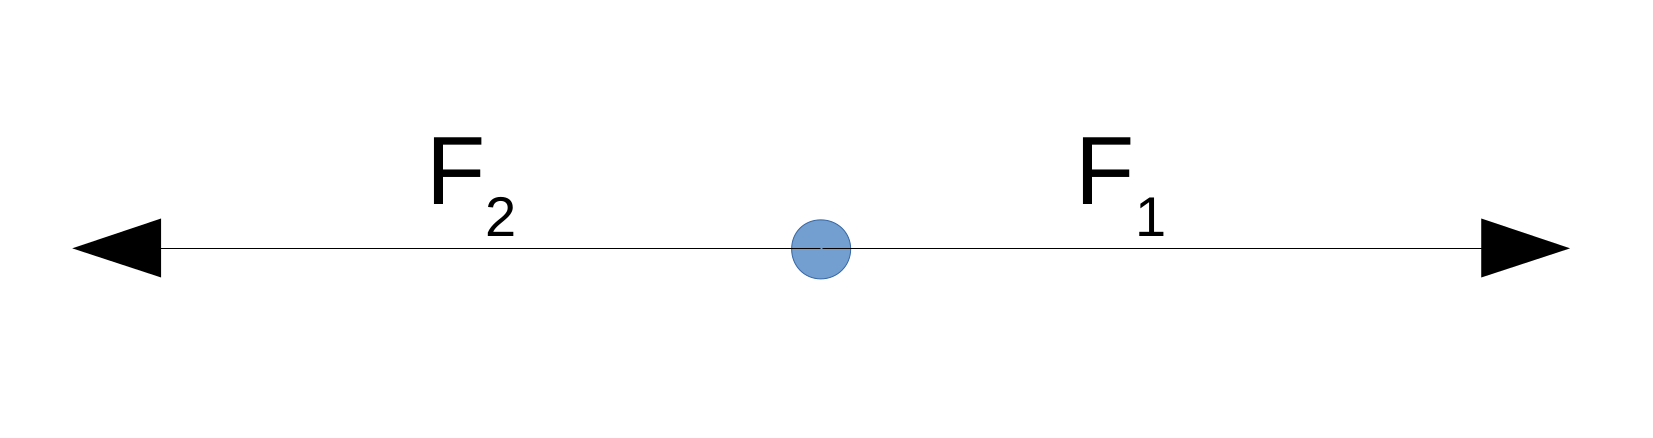
\includegraphics[width=0.7\textwidth]{kraefte_gleich}
	\caption{Gleich große, entgegengesetzte Kräfte: Es gibt keine resultierende Kraft.}
	\label{fig:kraefte_gleich}
\end{figure}

\noindent Bei zwei Kräften mit unterschiedlichem Betrag, die entgegengesetzt sind, müssen für den Betrag der Resultierenden die beiden Kräfte von einander abgezogen werden:

\begin{figure}[h!]
	\centering
	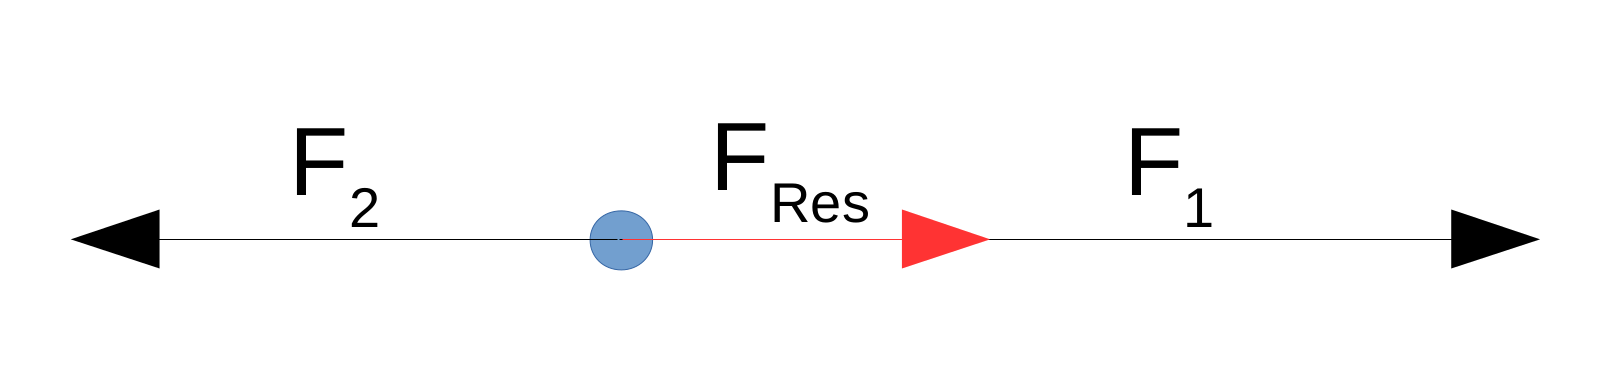
\includegraphics[width=0.7\textwidth]{kraefte_gleicherichtung}
	\caption{Entgegengesetzte Kräfte, mit unterschiedlichem Betrag.}
	\label{fig:kraefte_gleicherichtung}
\end{figure}

\subsubsection{Kräfte im rechten Winkel}

\noindent Die Pfeile von Kräften dürfen, z.B. zur erleichterten Herleitung von Gesetzen, verschoben werden, wenn ihre Länge und Richtung gewahrt werden. Dann wird kann der Fuß des einen Kraftpfeils an die Spitze des anderen Kraftpfeils angelegt und die Spitze zeigt dann die Spitze der Resultierenden an.

Dadurch ergibt sich aus dem Diagramm \ref{fig:kraefte_rechterwinkel} für zwei im rechten Winkel angreifende Kräfte mit dem Satz des Pythagoras:

\begin{align}
	F_{Res} = \sqrt{F_1^2 + F_2^2}
\end{align}

\begin{figure}[h!]
	\centering
	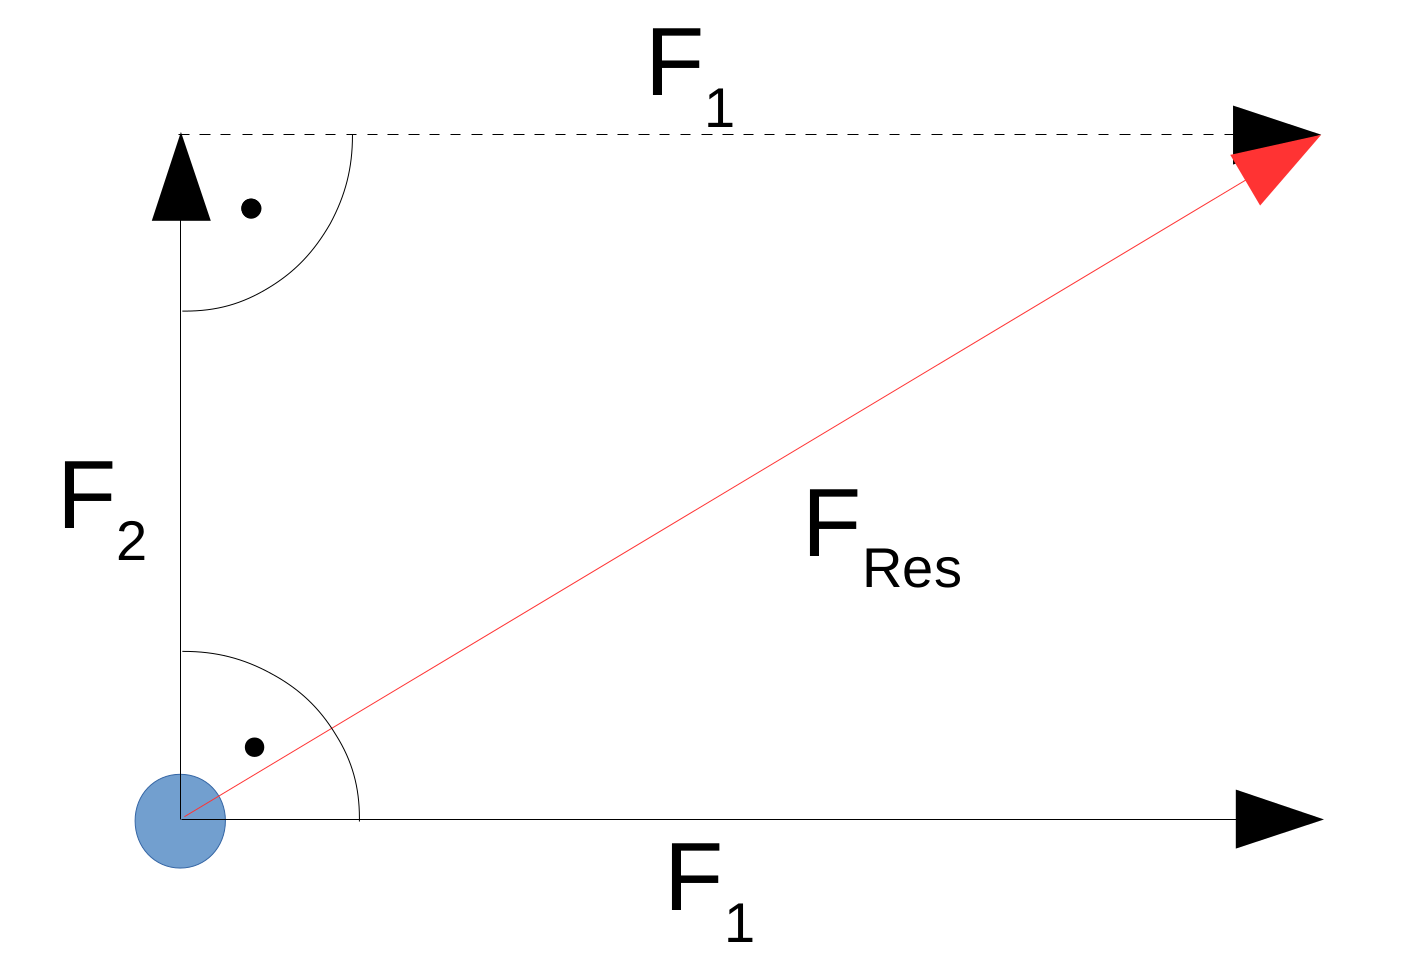
\includegraphics[width=0.7\textwidth]{kraefte_rechterwinkel}
	\caption{Kräfte im rechten Winkel}
	\label{fig:kraefte_rechterwinkel}
\end{figure}


\subsubsection{Kräfte im beliebigen Winkel}

\noindent Für einen beliebigen Winkel zwischen den Pfeilen muss mit dem Kosinussatz der Betrag der übrigen Seite $F_{Res}$ ermittelt werden, wie hier in Grafik \ref{fig:kraefte_beliebig}\endnote{Abbildungen \ref{fig:kraefte_beliebig}-\ref{fig:kraefte_gleich} \glqq Kräfteaddition\grqq{} von Till Blaha - Eigene Werke. Lizenziert unter Gemeinfrei}:

\begin{align}
	F_{Res} = \sqrt{F_1^2 + F_2^2 - 2F_1 F_2 \cdot \cos{\alpha '}}
\end{align}

\begin{figure}[H]
	\centering
	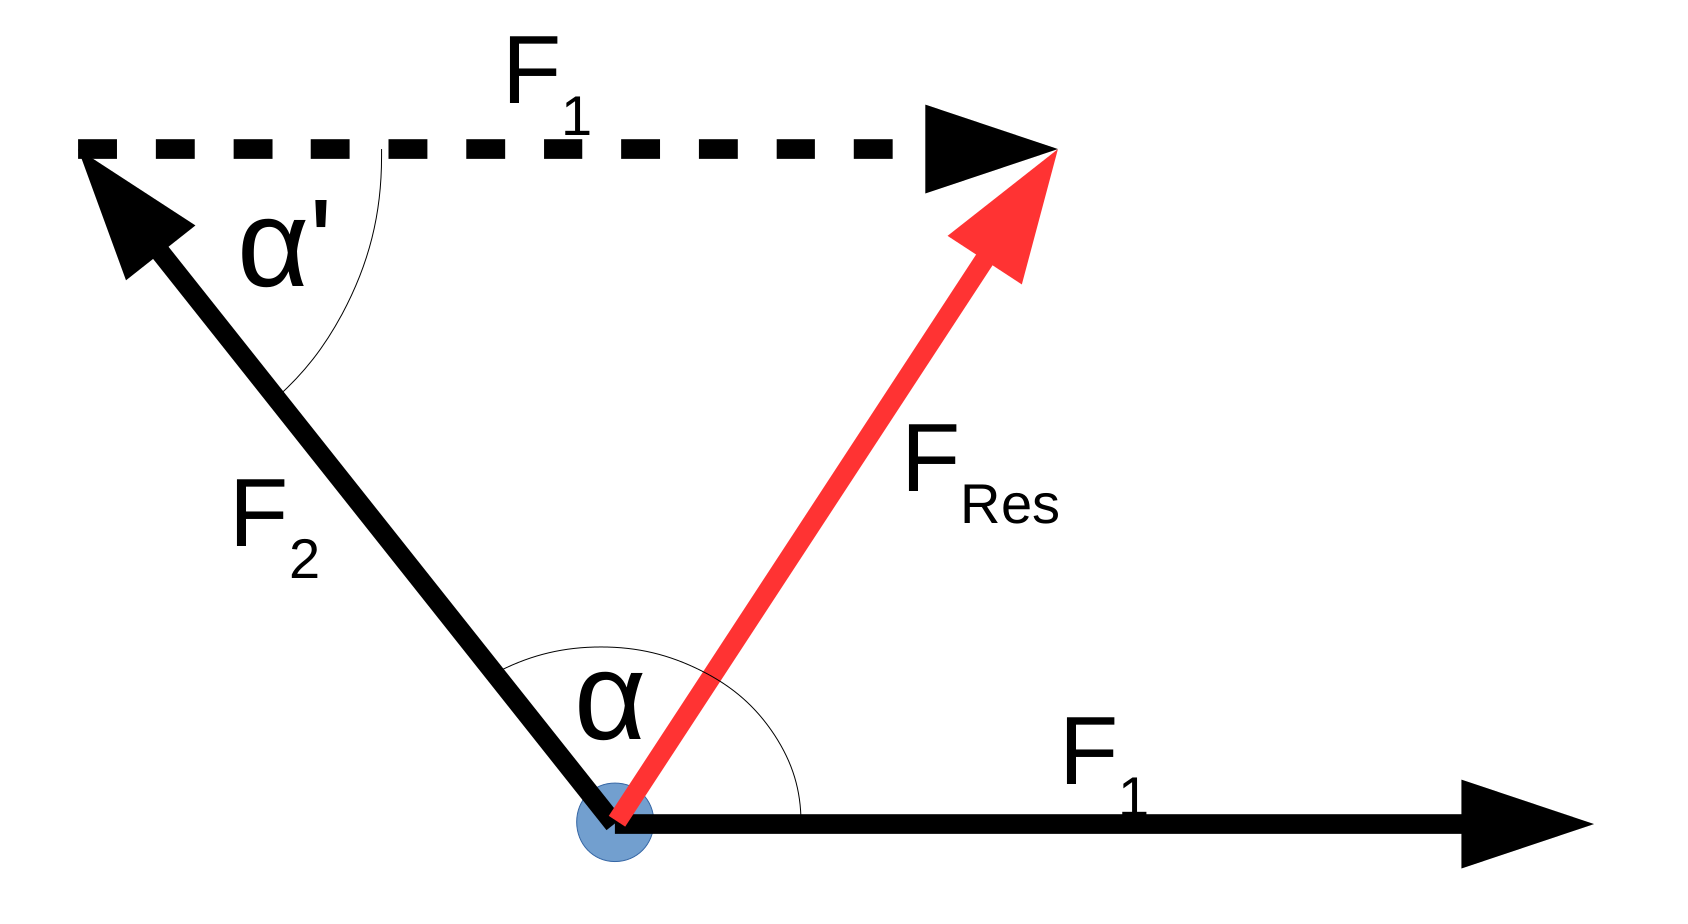
\includegraphics[width=0.7\textwidth]{kraefte_beliebig}
	\caption{Kräfte im beliebigen Winkel.}
	\label{fig:kraefte_beliebig}
\end{figure}


\subsection{Kräftesystem}

Aus dem dritten Newton'schen Axiom kann gefolgert werden, dass in einem abgeschlossenen Kräftesystem die Summe aller Kräfte $0$ sein muss, da jede Kraft eine gleich große und exakt entgegengesetzte Gegenkraft provoziert.

Dies ist wichtig für einige Herleitungen, z.B. am Federpendel (Siehe: \referenz{subsec:gesetze_federpendel}).


\subsection{Gewichtskraft} \label{subsec:Gewichtskraft}

Die Gewichtskraft $F_{G}$ ist die Kraft, die in der Mechanik besondere Bedeutung hat. Sie ist die Kraft, die ein Gravitationsfeld auf einen Körper auswirkt. Sie ist gemäß $F = m \cdot a$ abhängig von einer Beschleunigung, in diesem Fall der Gravitation (Schwerkraft) $g$, auf der Erde $\approx 9,81 \frac{m}{s^2}$, und von der Masse des Körpers:

\begin{align}
	F_{G} = m \cdot g
\end{align}

\noindent Die Einheit bleibt logischerweise das Newton.

\section{Energien} \label{sec:energien}
\begin{quote}
\glqq Energie ist eine Zustandsgröße von Körpern, die dessen Potential angibt, Arbeit zu verrichten.\grqq
\end{quote}

\subsection{Arbeit}

Die physikalische \glqq Arbeit\grqq{} (Formelzeichen $W$ von engl. \glqq Work\grqq ) ist definiert als Kraft mal Strecke, also wird Arbeit verrichtet wenn ein Körper über eine bestimmte Strecke hinweg von einer Kraft bewegt wird:

\begin{align}
	W = F \cdot s
\end{align}

\noindent Damit ergibt sich als Einheit der $Nm$ (sprich: \glqq Newtonmeter\grqq ) welcher auch als $J$ (sprich: \glqq Joule\grqq ).

\begin{Anmerkung}
Der Newtonmeter wird auch als Einheit für das Drehmoment verwendet, welches bei einer Drehbewegung die Kraft unter Berücksichtigung der Länge des Hebelarms angibt. Das Drehmoment hat aber als Größe nichts mit der Arbeit oder der Energie zu tun.
\end{Anmerkung}


\subsection{Energie}

\glqq Arbeit verrichten\grqq{} heißt Energie von einer Form in eine andere umzuwandeln. Daraus folgt, dass Energie im strengen Sinne nicht verloren gehen oder gewonnen werden kann, sie kann nur umgewandelt werden.

Die mathematische Definition der Energie ist daher dieselbe wie bei der Arbeit, nur dass das Formelzeichen $E$ ist; der Unterschied ist also ein rein philosophische Frage:

\begin{align}	\label{eq:energiedef}
	E = F \cdot s
\end{align}

\noindent Die Einheit ist ebenfalls $J$, in SI-Basiseinheiten $J=\frac{kg \cdot m^2}{s^2}$


\subsection{Energieerhaltung}

Aus dem Fakt, dass Energie nur in andere Formen umgewandelt werden kann, ergibt sich der Energieerhaltungssatz, der besagt, dass die Summe aller Energien in einem abgeschlossenen System konstant sein muss, egal wie viele Umwandlungen sich vollziehen, also egal, wie viel Arbeit verrichtet wird. 


\subsection{Energieformen}

Es gibt zwei wichtige Energieformen in der Mechanik:

\subsubsection{Potentielle Energie}

Die potentielle Energie, auch Lageenergie oder Höhenenergie genannt, besitzen Körper, die sich in einer Höhe, relativ zu einem Referenzsystem (beispielsweise die Höhe eines Körpers relativ zum Fußboden), befinden. Wenn die Masse des Körpers bekannt ist, ist die Energie nur noch abhängig von der Fallbeschleunigung, auch Gravität oder Schwerkraft genannt (Formelzeichen $g$) und der Höhe $h$. Auf der Erde beträgt die Fallbeschleunigung $\approx 9,81 \frac{m}{s^2}$.

Aus der allgemeinen Form für die Energie (Siehe \gleichungsreferenz{eq:energiedef}) und der Gewichtskraft $F_G = m \cdot g$ (Siehe \referenz{subsec:Gewichtskraft}) ergibt sich für $E_{pot}$:

\begin{align} \label{eq:epot}
	E_{pot} = m \cdot g \cdot h
\end{align}

\noindent Wenn dieser Körper nun fallen gelassen wird, wird diese potentielle Energie in kinetische Energie umgewandelt

\subsubsection{Kinetische Energie}

Kinetische Energie besitzen Körper, die bewegt sind. Sie ist abhängig von der Masse und von der Geschwindigkeit des Körpers:

\begin{align} \label{eq:ekin}
	E_{kin} = \frac{1}{2} m \cdot v^2
\end{align}

\begin{NiceToKnow}
	Die kinetische Energie ist das Integral nach der Geschwindigkeit des Impulses (Siehe: \referenz{subsub:impuls}): $E_{kin} = \int p \ dv = \int m \cdot v \ dv = \frac{1}{2} m \cdot v^2$
\end{NiceToKnow}

\subsection{Beispiel: Vorgänge beim Fall}

Fragestellung: Wenn ein Körper in einem luftleeren Raum (damit jegliche Luftreibung vernachlässigt werden kann) auf der Erde (damit gilt $g=9,81\frac{m}{s^2}$) aus $10m$ Höhe auf den Boden fällt, wie hoch ist seine Geschwindigkeit mit der er auf dem Boden auftrifft?

Ansatz: Bei diesem Vorgang wird potentielle Energie in kinetische Energie umgewandelt. Wenn der Körper bei Beginn des Falls ruhte, also keine Geschwindigkeit hatte, war dort die kinetische Energie $0$. Auf dem Boden angekommen, ist die Höhe des Körpers $0$, sodass die potentielle Energie dort ebenfalls $0$ ist. Daraus geht hervor, dass die potentielle Energie vollständig in kinetische umgewandelt wurde. Der Ansatz ist also, die beiden Gleichungen einander gleichzusetzen und dann nach $v$ umzustellen.

Anmerkung: Bei anfänglichem Betrachten der Gleichungen fällt auf, dass sie beide von $m$ abhängig sind, welches in der Fragestellung allerdings nicht gegeben ist. Das macht aber nichts, weil sich die Masse \glqq rauskürzt\grqq , wie man in der Umstellung sieht:

\begin{align}
\begin{split}
	E_{pot} &= E_{kin} \\
	mgh &= \frac{1}{2}m \cdot v^2 \\
	gh &= \frac{1}{2} \cdot v^2 \\
	2gh &= v^2 \\
	v &= \sqrt{2gh}
\end{split}
\end{align}

\noindent Mit eingesetzten Größen für $g$ und $h$:

\begin{align}
\begin{split}
	v &= \sqrt{2 \cdot 9,81 \cdot 10} \cdot \sqrt{\frac{m}{s^2} \cdot m} \\
	v &\approx 14 \frac{m}{s}
\end{split}
\end{align}

Die Einheitenrechnung, bei der Einheiten fast wie Variabeln betrachtet werden (bloß, dass für jede Einheit gilt: $U+U=U \neq 2U$) ergibt die Richtige Einheit $\frac{m}{s}$, was nochmal ein weiterer Ausschlag dafür ist, dass die Rechnung richtig war.






\section{Goldene Regel der Mechanik}
\begin{quote}
	\glqq Was man an Kraft spart, muss man an Weg zulegen.\grqq
\end{quote}

\noindent Diese einfache Regel bezieht sich auf jegliche mechanische Vorgänge bei denen Körper bewegt werden. Wenn man weniger Kraft aufwenden möchte, muss man den Körper über eine längere Strecke bewegen. 

Das einfachste Beispiel ist das heben eines Körpers. Dieser kann direkt hochgehoben werden, was eine Kraft erfordert, die größer ist, als die Kraft, die die Schwerkraft auf den Körper ausübt. Beispielsweise könnte der Körper aber auch über ein Rampe geschoben werden, welche dann den Weg, über welchen eine Kraft angewendet werden muss, vergrößert, aber die Kraft verkleinert. 

Wenn die Kraft $F$ ist und $s$ der Weg über welchen sie angewendet wird, gilt:

\begin{align}
	F_{1} \cdot s_1 = F_{2} \cdot s_2
\end{align}

\noindent Dies folgt direkt aus der Definition der Energie und dem Energieerhaltungssatz, da $E=F \cdot s$ (Siehe \referenz{sec:energien}).

\subsection{Flaschenzug}

Der Flaschenzug eignet sich sehr gut um diese Beziehung zu zeigen. Man betrachte folgende Abbildung\endnote{„Four pulleys“ von User:Prolineserver, User:Tomia. (minor edits by Stanisław Skowron, scale adjusted by User:Atropos235) - Eigenes Werk. Lizenziert unter CC BY 2.5 über Wikimedia Commons - \url{https://commons.wikimedia.org/wiki/File:Four_pulleys.svg}}:

\begin{figure}[h!]
	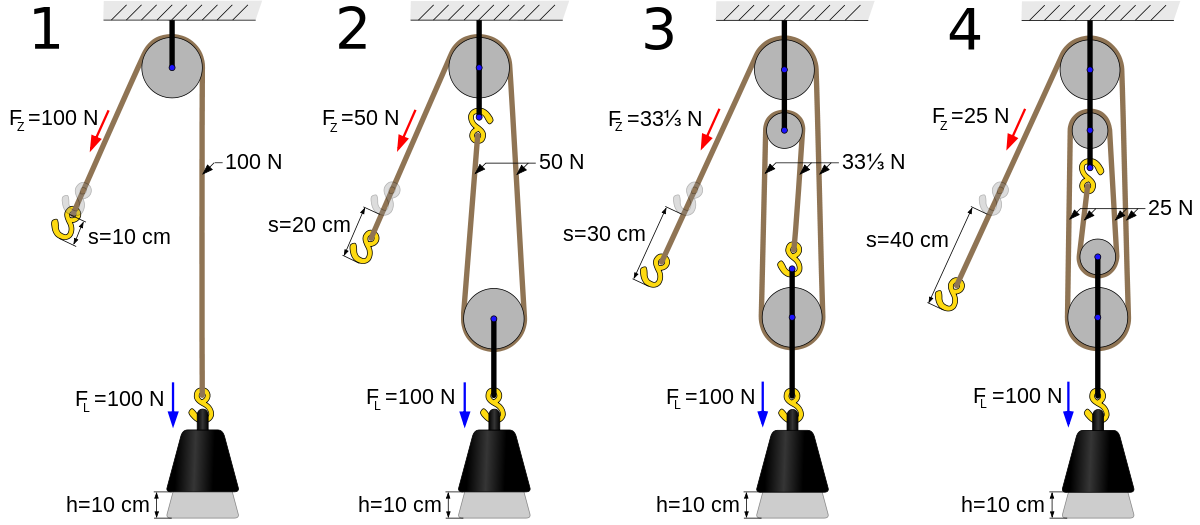
\includegraphics[width=\textwidth]{flaschenzug}
	\caption{4 Flaschenzüge, die dieselbe Last heben}
	\label{fig:flaschenzug}
\end{figure}

Die Last, die eine Gewichtskraft von $100N$ aufbringt, wird jedes Mal um $10cm$ angehoben, das heißt, dass die jeweilige Arbeit, die verrichtet wurde, konstant ist ($W = 100N \cdot 0,1m = 10J$).

Allerdings wird beim Addieren einer weiteren Rolle die Zahl der Seilstrecken, an denen quasi gleichzeitig gezogen wird, größer. Dadurch wird die zu ziehende Strecke $s$ proportional größer und die aufzuwendende Kraft $F_Z$ kleiner.



\section{Stöße}	\label{sec:stoesse}
Als Stöße bezeichnet man das Aufeinandertreffen von zwei Körpern unterschiedlicher Geschwindigkeiten. Das Ziel ist es, aus deren Massen und Geschwindigkeiten und der Art des Stoßes auf die Geschwindigkeiten \emph{nach} dem Stoß zu schließen.

\subsection{Impuls} \label{subsec:impuls}

Zur Beschreibung von Stößen muss vorerst noch eine weitere mechanische Größe eingeführt werden, der Impuls $p$. Der Impuls ist das Produkt aus Masse und Geschwindigkeit eines Körpers:

\begin{align}
	\vec{p} = m \cdot \vec{v}
\end{align}

\noindent Damit ist die Einheit des Impulses $\frac{kg \cdot m}{s} = Ns$ (sprich: \glqq Newtonsekunde\grqq).

\begin{NiceToKnow}
Der Impuls ist das zeitliche Integral der Kraft: $\int F \ dt = \int m \cdot a \ dt = m \cdot v$
\end{NiceToKnow}


\subsection{Elastischer Stoß}

Aus den zwei Stoßarten (elastisch und unelastisch) ist der elastische Stoß der ideale Stoß, bei dem keine Reibung zwischen den beiden aufeinandertreffenden Körpern stattfindet. In der Praxis geschieht das natürlich trotzdem, aber bspw. sind Stahlkugeln in guter Näherung reibungsfrei, sodass bei diesen und ähnlichen Versuchen von einem elastischen Stoß ausgegangen werden kann.

Da keine Energie durch Reibung in Wärme oder Verformung umgewandelt wird und somit \glqq verloren geht\grqq , muss neben dem Impuls auch die Energie erhalten bleiben, also während des Versuches konstant sein. Daher gestaltet sich die Herleitung für eine Gleichung, die die Geschwindigkeiten nach dem Stoß voraussagt, recht komplex; beide Sätze müssen berücksichtigt werden. Daher wird hier dieses Gesetz nur genannt:

Wenn ein Körper mit der Masse $m_1$ und der Geschwindigkeit $v_1$ auf einen zweiten Körper mit der Masse $m_2$ und der Geschwindigkeit $v_2$ unter den Voraussetzungen eines elastischen Stoßes aufeinander treffen, gilt für die Geschwindigkeit des zweiten Körpers nach dem Stoß $v_2'$:

\begin{align}
\begin{split}
	v_2'=\frac{m_2 \cdot v_2 + m_1(2v_1 - v_2)}{m_1 + m_2}
\end{split}
\end{align}

\noindent Für $v_1'$ gilt dann:

\begin{align}
\begin{split}
	v_1'=\frac{m_1 \cdot v_1 + m_2(2v_2 - v_1)}{m_1 + m_2}
\end{split}
\end{align}


\subsection{Unelastischer Stoß}

Bei einem unelastischen Stoß geht ein Teil der kinetischen Energie der zwei Stoßkörper in Wärme oder Verformung \glqq verloren\grqq , dass heißt sie steckt nachher nicht mehr in der kinetischen Energie der Körper. 

Bei einem perfekt unelastischen Stoß, bei dem die beiden Körper sich \glqq verkeilt\grqq{} zusammen mit der selben Geschwindigkeit fortbewegen. 

Der Impulserhaltungssatz muss trotzdem erhalten bleiben und aus diesem geht für $v'$ nach dem Stoß hervor:

\begin{align}
\begin{split}
	p' &= p_1 + p_2 \\
	v'(m_1 + m_2) &= v_1 \cdot m_1 + v_2 \cdot m_2 \\
	v' &= \frac{v_1 \cdot m_1 + v_2 \cdot m_2}{m_1 + m_2}
\end{split}
\end{align}



\section{Bewegungsgesetze} \label{sec:bewegungsgesetze}
Die Gesetze der Bewegung, auch Translation genannt, ist ein wiederkehrendes Thema in der Physik. Die Gesetze beschreiben die Bewegung von Körpern und geben deren Ort in Abhängigkeit einer Variablen, meistens der Zeit, an:

\subsection{Gleichförmige Bewegung} \label{subsec:gleichfoermig}

Die gleichförmige Bewegung ist eine Bewegung, die nicht beschleunigt ist; der Körper bewegt sich mit einer konstanten Geschwindigkeit fort. Daher gilt für die insgesamt zurückgelegte Strecke $s$:

\begin{align} \label{eq:gleichfoermig}
	s(t) = v \cdot t + s_0
\end{align}

\begin{figure}[h!]
	\centering
	\begin{minipage}[b]{0.45\linewidth}
		\begin{comment} Gnuplot:
set xlabel "t"
set ylabel "s(t)"
set output "plot_bewegung_gleichfoermig_s.png"
plot s(x) = 1x ls 1
		\end{comment}
    	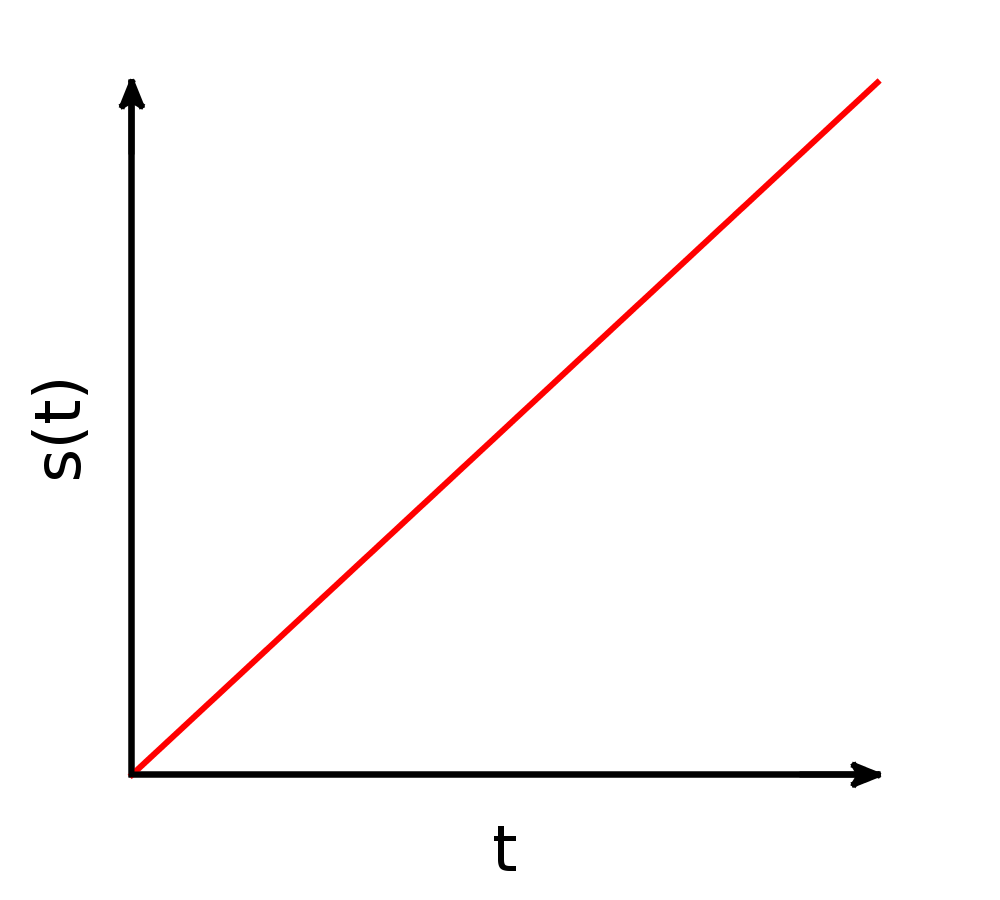
\includegraphics[width=\textwidth]{plot_bewegung_gleichfoermig_s}
	\end{minipage}
	\begin{minipage}[b]{0.45\linewidth}
		\begin{comment} Gnuplot:
set xlabel "t"
set ylabel "v(t)"
set output "plot_bewegung_gleichfoermig_v.png"
plot 1 ls 1
		\end{comment}
    	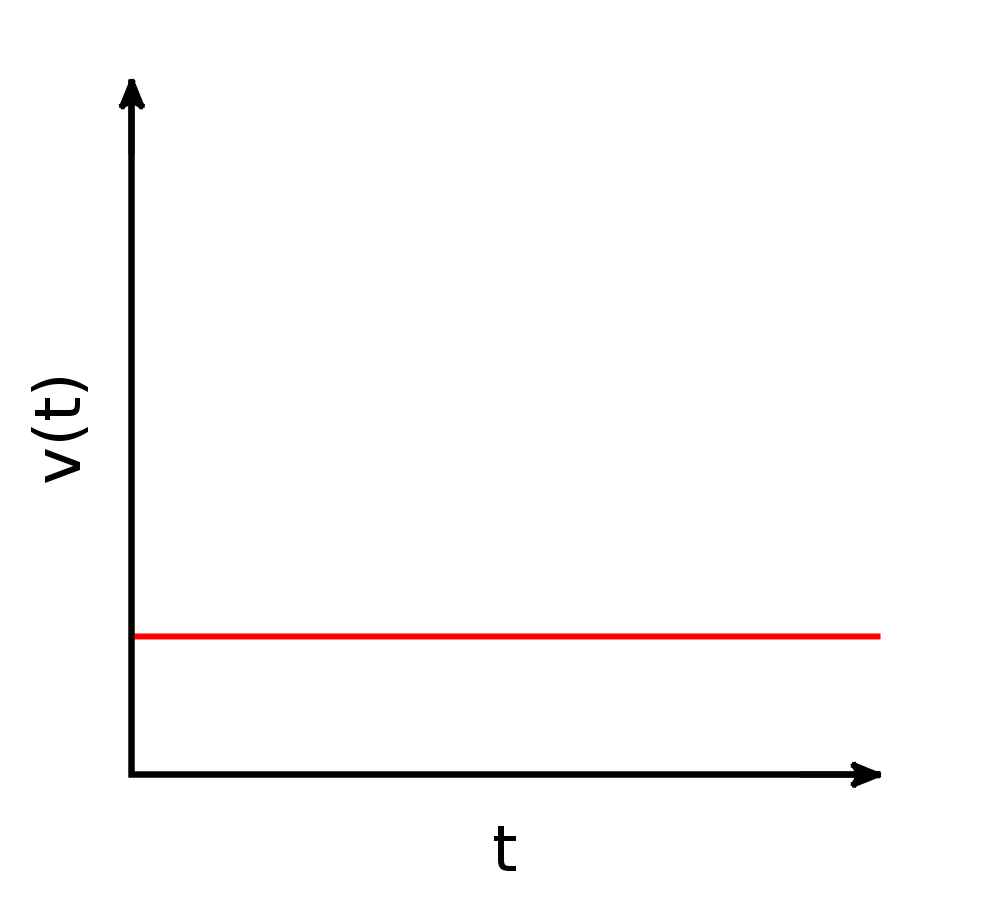
\includegraphics[width=\textwidth]{plot_bewegung_gleichfoermig_v}
	\end{minipage}
	\caption{Gleichförmige Bewegung: Beziehung zwischen Weg und Geschwindigkeit}
\end{figure}


\begin{Wichtig}
$v$ ist konstant!
\end{Wichtig}

\noindent Dabei ist $s_0$ die Anfangsstrecke, die schon zu Beginn, bevor die Translation betrachtet wird, zurückgelegt wurde.

\begin{figure}[h!]
	\centering
	\begin{comment} Gnuplot:
set xlabel "t"
set ylabel "s(t)+s_0"
set output "plot_bewegung_gleichfoermig_s+s0.png"
plot s(x) = 1x+1 ls 1
	\end{comment}
	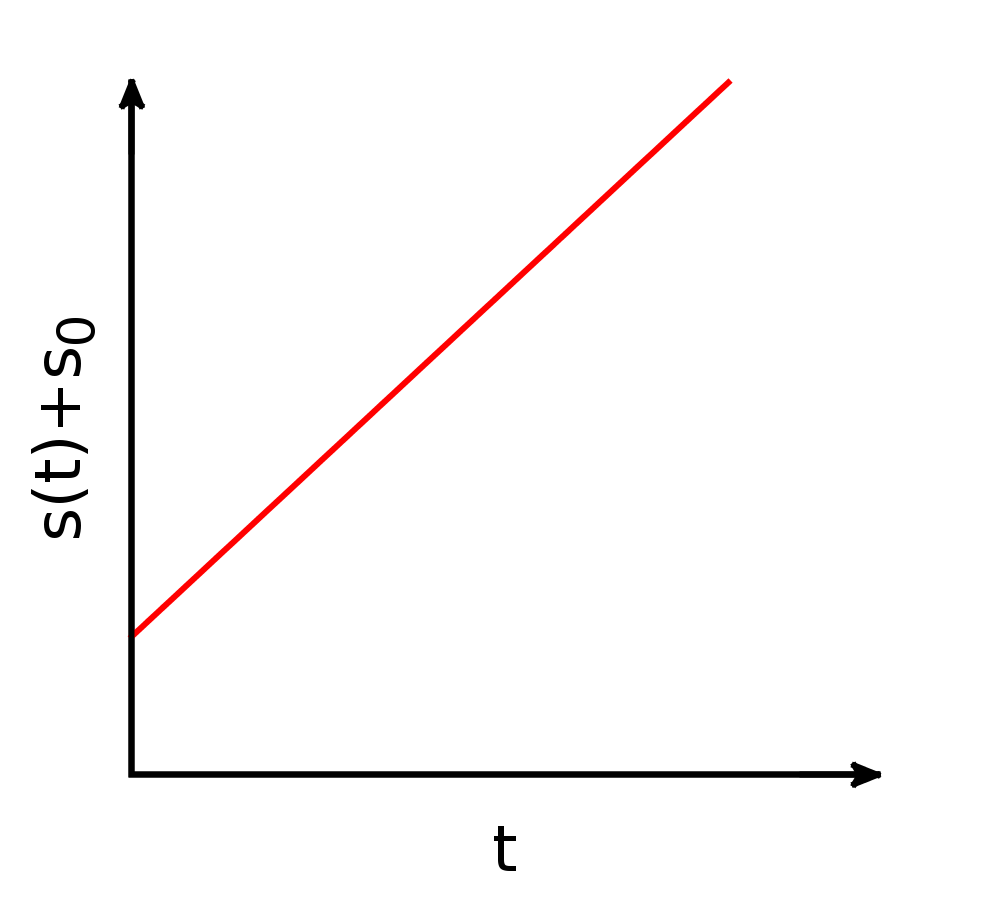
\includegraphics[width=0.6\textwidth]{plot_bewegung_gleichfoermig_s+s0}
	\caption{Mit Anfangsgeschwindigkeit: Der Graph ist verschoben}
\end{figure}

\subsection{Gleichmäßig beschleunigte Bewegung}

Eine Bewegung kann auch mit einer sich ändernden Geschwindigkeit von statten gehen. Sollte diese Beschleunigung konstant sein, nennt man diese Bewegung gleichmäßig beschleunigte Bewegung.

\subsubsection{Gesamtstrecke}

Bei dieser Bewegung lässt sich die Durchschnittsgeschwindigkeit über den Zeitraum $t$ mit $\frac{1}{2}a \cdot t$ berechnen, da die Endgeschwindigkeit $a \cdot t$ ist: Die Änderung der Geschwindigkeit $a$, angewandt über den Zeitraum $t$, resultiert in der Endgeschwindigkeit. Da die Beschleunigung konstant ist und damit die Geschwindigkeit proportional zur Zeit, ist der Faktor, der zur gemittelten Geschwindigkeit führt $\frac{1}{2}$.

Dann kann dieses $\frac{1}{2}a \cdot t$ für das $v$ im ersten Glied der Gleichung \ref{eq:gleichfoermig} eingesetzt werden und man erhält die Bewegungsgleichung für die gleichmäßig beschleunigte Bewegung:

\begin{align} \label{eq:streckegleichmaessig}
	s(t) = \frac{1}{2}a \cdot t^2 + v_0 \cdot t + s_0
\end{align}

\begin{figure}[h!]
	\centering
	\begin{minipage}[b]{0.32\linewidth}
		\begin{comment} Gnuplot:
set xlabel "t"
set ylabel "s(t)"
set output "plot_bewegung_beschleunigt_s.png"
plot 0.5 * 1 * x * x ls 1
		\end{comment}
    	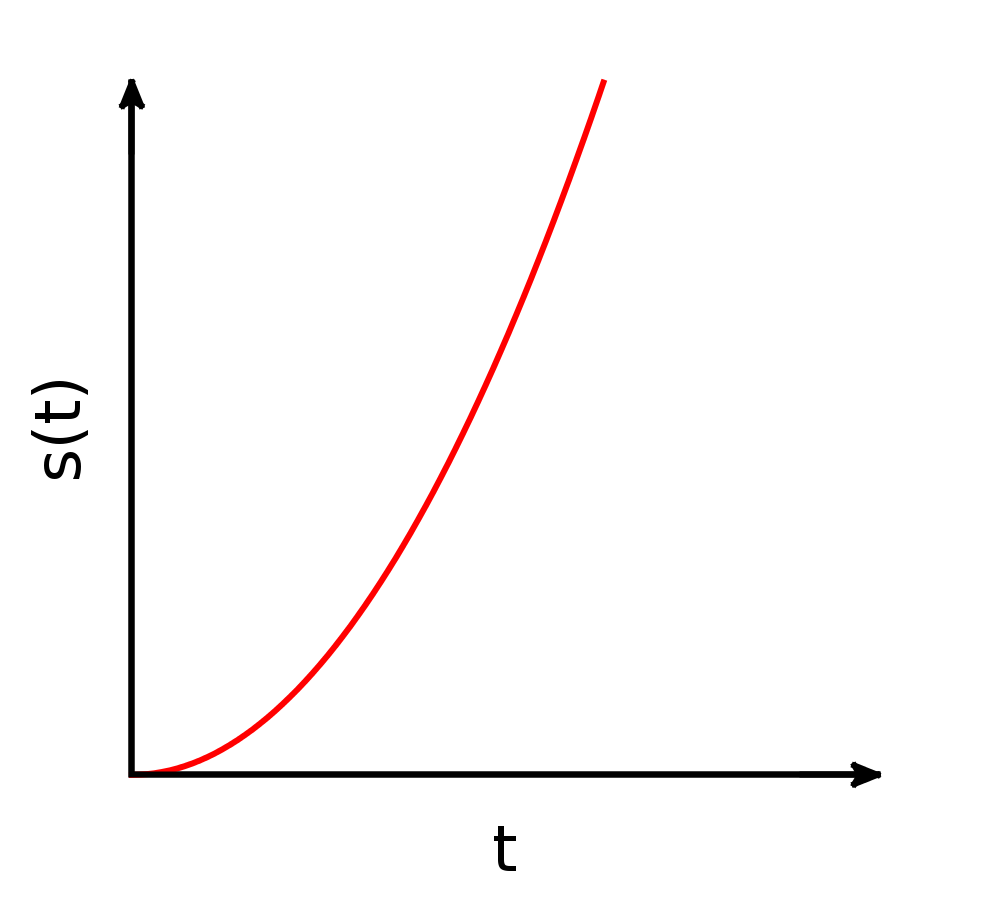
\includegraphics[width=\textwidth]{plot_bewegung_beschleunigt_s}
	\end{minipage}
	\begin{minipage}[b]{0.32\linewidth}
		\begin{comment} Gnuplot:
set xlabel "t"
set ylabel "v(t)"
set output "plot_bewegung_beschleunigt_v.png"
plot x ls 1
		\end{comment}
    	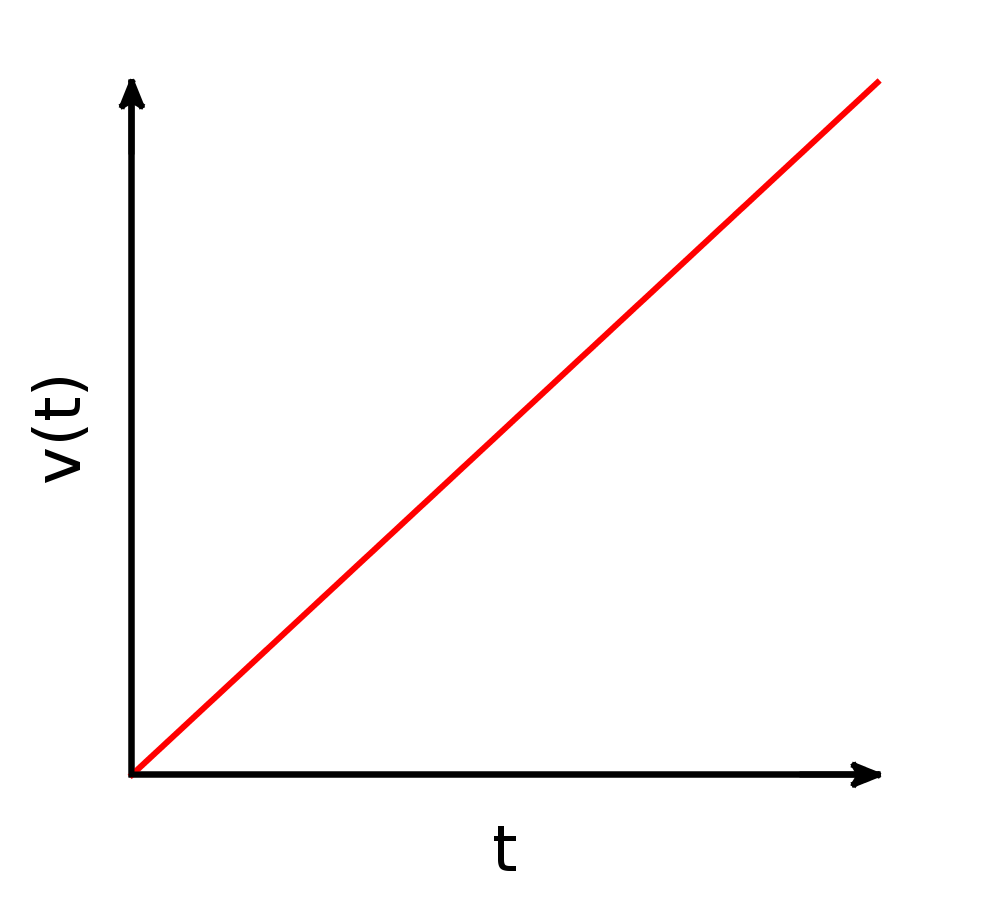
\includegraphics[width=\textwidth]{plot_bewegung_beschleunigt_v}
	\end{minipage}
	\begin{minipage}[b]{0.32\linewidth}
		\begin{comment} Gnuplot:
set xlabel "t"
set ylabel "a(t)"
set output "plot_bewegung_beschleunigt_a.png"
plot 1 ls 1
		\end{comment}
    	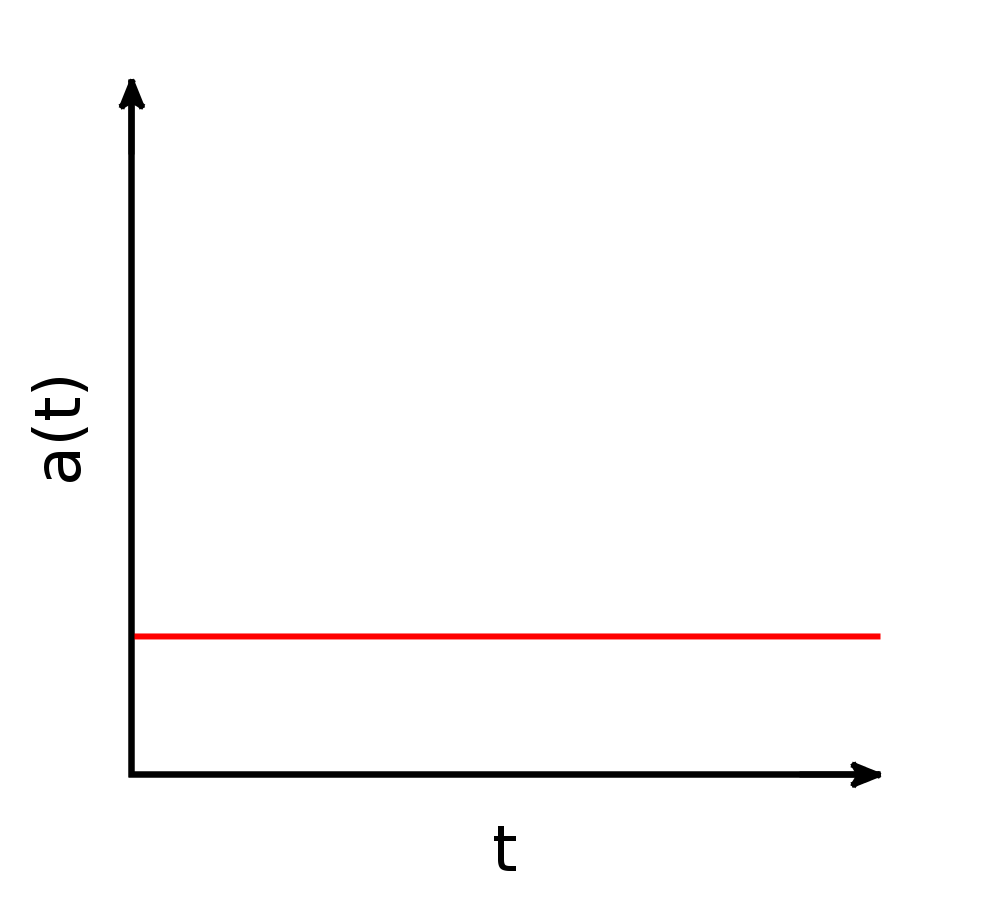
\includegraphics[width=\textwidth]{plot_bewegung_beschleunigt_a}
	\end{minipage}
	\caption{Gleichmäßig beschleunigte Bewegung: Beziehung zwischen Weg, Geschwindigkeit und Beschleunigung}
	\label{fig:beschleunigt}
\end{figure}

\noindent Neben der Anfangsstrecke $s_0$ kommt nun aber auch noch die Anfangsgeschwindigkeit $v_0$ dazu, die von Belang ist, wenn man einen Fall hat, bei dem der Körper vor Einwirkung der Beschleunigung schon eine Geschwindigkeit $>0$ hatte.


\subsubsection{Endgeschwindigkeit}

Wie schon angesprochen, ist die Endgeschwindigkeit proportional zur verstrichenen Zeit. Was aber dort noch nicht berücksichtigt wurde, ist, dass auch für die Endgeschwindigkeit nach der verstrichenen Zeit $t$ die Anfangsgeschwindigkeit $v_0$ eine Rolle spielt:

\begin{align}	\label{eq:geschwindigkeitgleichmaessig}
	v(t) = a \cdot t + v_0
\end{align}

\noindent Dies ist die zeitliche Ableitung der Gleichung \ref{eq:streckegleichmaessig}


\subsubsection{Beziehungen über die Ableitungen}

Würde man noch eine Ableitung der Gleichung \ref{eq:geschwindigkeitgleichmaessig} machen bekäme man die Gleichung für die Beschleunigung. Das wäre aber witzlos, da die Beschleunigung einer gleichmäßig beschleunigten Bewegung konstant ist und damit $s''(t)=v'(t)=a(t)=a= const.$ ist.

Dennoch ist es hilfreich, diese Beziehungen im Kopf zu haben (Man beziehe auch Abbildung \ref{fig:beschleunigt}):

\begin{align}
\begin{split}
	s'(t) &= v(t) \\
	v'(t) &= a \\
	s''(t) &= v'(t)= a
\end{split}
\end{align}

\noindent Die Ableitung des Weges, also die zeitliche Änderung des Weges, ist die Geschwindigkeit. Die zeitliche Änderung der Geschwindigkeit ist die Beschleunigung. Daher ist die zeitliche Änderung der zeitlichen Änderung des Weges, die Beschleunigung.





\section{Würfe}
Bei der Beschreibung von Würfen, also von Flugbahnen von Körpern, wendet man die Bewegungsgesetze an und kombiniert diese falls notwendig.


\subsection{Vertikaler Wurf}

Der vertikale Wurf ist eine eindimensionale Bewegung, bei der ein Körper mit einer bestimmten Geschwindigkeit senkrecht nach oben geworfen wird und durch die Erdbeschleunigung wieder nach unten beschleunigt wird.

Daher lässt sich die Bewegung mit der \gleichungsreferenz{eq:streckegleichmaessig} ausdrücken:

\begin{align} \label{eq:wurfvertikal}
	h(t) = -\frac{1}{2}g \cdot t^2 + v_0 \cdot t + h_0
\end{align}

\noindent Diese Gleichung kann gleich $0$ gesetzt werden um den Zeitpunkt zu erhalten, bei dem der Körper wieder auf der Erde aufschlägt. Um die Geschwindigkeit, mit der der Körper auftrifft zu erhalten, muss der errechnete Zeitpunkt in die Gleichung für die Geschwindigkeit (Siehe: \gleichungsreferenz{eq:geschwindigkeitgleichmaessig}) für $t$ und die negative Erdbeschleunigung ($-g$) für $a$ eingesetzt werden.


\subsection{Waagerechter Wurf}

Der waagerechte Wurf tritt bspw. ein, wenn ein Flugzeug Ladung abwirft.

Die Bewegung des Ladungskörpers in x-Richtung, also entlang der Flugrichtung, verläuft gleichförmig (Luftreibung wird ignoriert), also mit konstanter Geschwindigkeit. Die Bewegung in y-Richtung ist, wie beim vertikalen Wurf eine gleichmäßig beschleunigte Bewegung mit der Erdbeschleunigung.

Folgende zwei Gleichungen sind zur Beschreibung nötig, wobei nicht mehr $s$, sondern $x$ und $h$ (Höhe) für die Strecken verwendet werden, da es ja nun 2 Richtungen gibt:

\begin{align}
	x(t) = v_x \cdot t
\end{align}

\begin{align}
	h(t) = -\frac{1}{2}g \cdot t^2 + h_0
\end{align}

\noindent Bei $x(t)$ wurde absichtlich die mögliche Anfangsstrecke weggelassen, zur Vereinfachung der weiteren Rechnung.

Nun ist es praktisch, nur eine Gleichung für die Beschreibung einer Bewegung zu haben. Dafür wird $x(t)$ nach $t$ umgestellt und dieses $t$ dann in $h(t)$  eingesetzt, sodass man eine Gleichung für die Höhe in Abhängigkeit von der Strecke in x-Richtung hat, was oft deutlich handlicher ist, als eine Gleichung für $h$ in Abhängigkeit der Zeit:

\begin{align}
\begin{split}
	x(t) &= v_x \cdot t \\
	t(x) &= \frac{x}{v_x}
\end{split}
\end{align}

\noindent Eingesetzt in $h(t)$:

\begin{align} \label{eq:waagerechtgesamt}
\begin{split}
	h(t) &= -\frac{1}{2}g \cdot t^2 + h_0 \\
	h(x) &= -\frac{1}{2}g \cdot \frac{x^2}{v_x^2} + h_0
\end{split}
\end{align}


\subsection{Schiefer Wurf}

Beim schiefen Wurf wird ein Körper unter einem Winkel geworfen, sodass dieser eine Wurfparabel beschreibt.

Der schiefe Wurf ist prinzipiell dieselbe Kombination aus beiden Bewegungsarten wie beim waagerechten Wurf, aber mit der Schwierigkeit, dass aus dem Abwurfwinkel $\alpha$ und der Abwurfgeschwindigkeit $v_0$ erst die Anfangsgeschwindigkeiten in die beiden Richtungen, $v_x$ in Richtung des Wurfes und $v_y0$ in die Höhe, berechnet werden müssen. Die Anfangsgeschwindigkeit in y-Richtung wird deshalb nicht einfach $v_y$ genannt, weil sie, im Gegensatz von $v_x$, im Laufe des Wurfes variiert:
%Cue for pic of triagle

\begin{align}
\begin{split}
	\cos{\alpha} &= \frac{v_x}{v_0} \\
	v_x &= \cos{\alpha} \cdot v_0
\end{split}
\end{align}

\begin{align}
\begin{split}
	\sin{\alpha} &= \frac{v_{y0}}{v_0} \\
	v_{y0} &= \sin{\alpha} \cdot v_0
\end{split}
\end{align}

\noindent Damit können die Bewegungsgesetze eingefüllt werden:

\begin{align}
\begin{split}
	x(t) &= v_x \cdot t \\
	x(t) &= \cos{\alpha} \cdot v_0 \cdot t
\end{split}
\end{align}

\begin{align}
\begin{split}
	y(t) &= -\frac{1}{2}g \cdot t^2 + v_{y0} \cdot t + y_0 \\
	y(t) &= -\frac{1}{2}g \cdot t^2 + \sin{\alpha} \cdot v_0 \cdot t + y_0
\end{split}
\end{align}


\subsubsection{Gesamtgleichung}


Jetzt kann wieder $t$ in $y(t)$ mit der nach $t$ umgestellten Gleichung für $x(t)$ ersetzt werden und man erhält die Gesamtgleichung.

\begin{align}
\begin{split}
	x(t) &= \cos{\alpha} \cdot v_0 \cdot t \\
	t(x) &= \frac{x}{\cos{\alpha} \cdot v_0}
\end{split}
\end{align}

\noindent Einsetzen:

\begin{align}
\begin{split}
	y(t) &= -\frac{1}{2}g \cdot t^2 + \sin{\alpha} \cdot v_0 \cdot t + y_0 \\
	y(x) &= -\frac{1}{2}g \cdot \frac{x^2}{\cos{^2\alpha} \cdot v_0^2} + \sin{\alpha} \cdot v_0 \cdot \frac{x}{\cos{\alpha} \cdot v_0} + y_0 \\
	y(x) &= -\frac{1}{2}g \cdot \frac{x^2}{\cos{^2\alpha} \cdot v_0^2} + \frac{\sin{\alpha} \cdot v_0 \cdot x}{\cos{\alpha} \cdot v_0} + y_0 \\
	y(x) &= -\frac{1}{2}g \cdot \frac{x^2}{\cos{^2\alpha} \cdot v_0^2} + \tan{\alpha} \cdot x + y_0 \\
\end{split}
\end{align}

\noindent Diese Gesamtgleichung kann nun zur Berechnung benutzt werden, z.B. zur Wurfweitenbestimmung muss die Gleichung gleich $0$ gesetzt werden, etc.:

\begin{align}
\begin{split}
	y(x) &= \tan{\alpha} \cdot x - \frac{g \cdot x^2}{2\cos{^2\alpha} \cdot v_0^2} + y_0
\end{split}
\end{align}

\section{Kreisbewegung}
Die Gesetze der Kreisbewegung beschreiben einen Körper, der sich mit einer konstanten Geschwindigkeit auf einer Kreisbahn mit konstantem Radius bewegt.


\subsection{Frequenz}

Die Frequenz $f$ bezeichnet die Anzahl an Kreisumläufen pro Zeiteinheit. Die Einheit ist $Hz$ (sprich: \glqq Hertz\grqq ), also $\frac{1}{s}$.

Die Dauer \emph{eines} Kreisumlaufes nennt man auch die Periodendauer $T$. Dann gilt:

\begin{align}
	f = \frac{1}{T}
\end{align}

\subsection{Winkelgeschwindigkeit}

Die Winkelgeschwindigkeit gibt an, wie groß der Umfangsabschnitt ist, der in einer bestimmten Zeit absolviert wird:

\begin{align}
	\omega = 2 \pi f = \frac{2 \pi}{T}
\end{align}

\noindent Die Einheit ist $\frac{rad}{s}$ (sprich: \glqq Radiant pro Sekunde\grqq ) und ein Umlauf entspricht $2\pi$.

\begin{Wichtig}
Das Formelzeichen $\omega$ ist \glqq klein Omega\grqq{} und nicht \glqq w\grqq .
\end{Wichtig}


\subsection{Bahngeschwindigkeit im Kreis}

Die Bahngeschwindigkeit gibt in absoluten Einheiten ($\frac{m}{s}$) an, wie schnell sich das Objekt auf der Bahn fortbewegt. Zusätzlich zur Winkelgeschwindigkeit, muss bei der Kreisbahn daher noch der Radius bekannt sein:

\begin{align} \label{eq:bahngeschwindigkeit}
	v=\omega r= 2r\pi f = \frac{2r\pi}{T}
\end{align}

Eine andere Herleitung aus dem Kreisumfang $U=2r\pi$, der Periodendauer $T$ und der generellen Formel für Bahngeschwindigkeit $v=\frac{s}{t}$ könnte wie folgt Aussehen:

\begin{align}
	v &=\frac{s}{t} \\
	v &=\frac{2r\pi}{T}
\end{align}


\subsection{Zentripetalbeschleunigung}
%Cue for herleitung
Um auf einer Kreisbahn zu bleiben, muss eine Zentripetalbeschleunigung auf einen Körper wirken, die zum Kreiszentrum hin zeigt. Die Formel lautet:

\begin{align}
	a_z=\frac{v^2}{r}=\omega^2 r
\end{align}

Eine tolle Herleitung findet sich \href{http://www.schule-bw.de/unterricht/faecher/physik/online\_material/mechanik2/kreis/zentripetalkraft.htm}{hier}\footnote{\url{http://www.schule-bw.de/unterricht/faecher/physik/online_material/mechanik2/kreis/zentripetalkraft.htm}}.

\subsection{Zentripetalkraft}

Dies ist die Kraft, die auf einen Körper ausgewirkt werden muss, damit er auf einer Kreisbahn bleibt. Zusätzlich zur Zentripetalbeschleunigung muss nun also noch gemäß Newtons zweiten Axiom $F=a \cdot m$ die Masse als Faktor in die Gleichung aufgenommen werden:

\begin{align}
	F_z &= a_z \cdot m \\
	F_z &= \frac{v^{2}m}{r}
\end{align}



\chapter{Elektrisches Feld} \label{ch:EFeld}
\section{Beweis für die Existenz}

%%%%% Elektrisches Feld %%%%%
%% #1 Beweis %%


%Some sample text to be displayed above the first subsection

%\subsection{Prinzip}

%Ein Zyklotron besteht aus Zwei hohlen, halbzylindrischen und Duanden an denen eine Spannung mit unterschiedlichem Vorzeichen anliegt, und darüber bzw. darunter liegende Magneten, die ein homogenes Magnetfeld erzeugen. Zudem gibt es einen Einlass und einen Auslass für Teilchen.

%\begin{wrapfigure}{r}{0.4\textwidth} \label{Zyklo}
%
%	\vspace{-10pt}
%	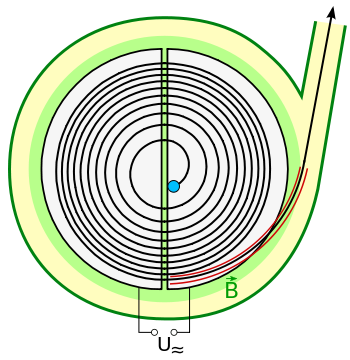
\includegraphics[width=0.35\textwidth]{Zyklotron_Prinzipskizze02.png}
%	\vspace{-13pt}
%	\caption{Prinzipskizze eines Zyklotrons}
%	\vspace{-5pt}	
%	
%\end{wrapfigure}

%\subsubsection{Anwendung}

% Some Formula:

%\begin{equation}
%	x= \frac{y \cdot 13 \pi z}
%			{\cos \alpha}
%\end{equation}

%%%%%%%%%%%%%%%%%%%%%%%
% Eigentlicher Beginn %
%%%%%%%%%%%%%%%%%%%%%%%

\subsection{Elektrostatik}

Wenn ein Körper geladen ist, bedeutet das, dass auf diesem positive und negative Ladungen in ungleich großen Mengen vorhanden sind. Daraus folgt, dass sich gleichgroße Mengen ungleichnamiger (positiv $\neq$ negativ) Ladungen neutralisieren.

Gleichnamige Landungen stoßen sich ab, während ungleichnamige Ladung sich anziehen. Dies ähnelt sehr dem magnetischen Feld (Siehe \ref{ch:MFeld}) und steht Gravitationsfeldern entgegen, welche sich ausschließlich gegenseitig anziehen.

In Metallen sind die negativen Ladungen beweglich, sie heißen Elektronen. Diese Eigenschaft macht Metalle zu \glqq Leitern\grqq .

\begin{NiceToKnow}
Der Begriff Elektron (und alle davon abgeleitete Begriffe) kommt vom altgriechischen Wort \glqq élektron\grqq{} und bedeutet \glqq Bernstein\grqq . Der Effekt der Ladung wurde schon im alten Griechenland an Bernstein entdeckt.
\end{NiceToKnow}


\subsection{Elektroskop}

Ein Elektroskop besteht im Kern aus einer Schnecke aus Metallband. Ein Zeiger, der an der Schnecke befestigt ist, schlägt aus, sobald es einen Überschuss an positiver oder negativer Ladung gibt, da sich dann durch die gleichnamige Ladungen die vielen Windungen gegenseitig voneinander abstoßen.


\subsection{Influenz} \label{subsec:Influenz}

Nun ist es logisch, dass bei Berührung eines Elektroskops mit einem negativ geladenen Körper, die Nadel ausschlägt, da das Metallband diese Elektronen leitet und ein Überschuss an negativer Ladung in der Schnecke zum Ausschlag führt.

Aber auch wenn ein beliebig geladener Körper (beispielsweise ein positiv geladener Kunststoffstab) nur über das Elektroskop gehalten wird, ohne es zu berühren, schlägt die Nadel aus. Dies nennt man \emph{Influenz} und das Phänomen beruht darauf, dass sich ungleichnamige Ladungen anziehen. Die beweglichen negativen Ladungen wandern durch die Anziehung des positiven Kunststoffstabs weg von der Schnecke und hinterlassen dort einen Überschuss an positiven Ladungen, sodass die Nadel ausschlägt. Entfernt man den Stab wieder, gelangt der Zeiger wieder in die Ausgangslage.

Das Besondere dabei ist, dass diese Influenz kein Medium benötigt, also auch im Vakuum über Distanzen auftritt. Damit ist ein Feldcharakter bewiesen.

\begin{Anmerkung}
Eigentlich sind nur negative Ladungen in einem Leiter beweglich, nämlich die Elektronen. Trotzdem spricht man manchmal davon, dass sich positive Ladungen von A nach B bewegen. Grundsätzlich bewegen sich dabei aber die negativen Ladungen von B nach A, sodass auf der Seite von B ein Defizit negativer Ladungen auftritt, diese Seite also positiv geladen ist.

Daher kann man von wandernden positiven Ladungen sprechen, da das Ergebnis dasselbe ist; die Mechanik dahinter ist jedoch eine Andere.
\end{Anmerkung}


\section{Modellierung und Mathematisierung}

Um das Phänomen der Influenz und vieles Weitere rund um die Elektrizität zu beschreiben, wurde das Modell des elektrischen Feldes entwickelt. 

\begin{NiceToKnow}
Generell geht es in der Physik nicht unbedingt darum, zu erläutern, wie etwas genau funktioniert, da vieles, wie zum Beispiel die eigentliche Beschaffenheit von Feldern, (noch) gar nicht genau zu erklären ist. Es geht darum, Modelle zu entwickeln, mit deren Hilfe sich mathematische Ausdrücke zur Beschreibung von diesen Phänomenen ableiten lassen.
\end{NiceToKnow}


\subsection{Feldlinien}

\begin{figure}[h!]
	\centering
	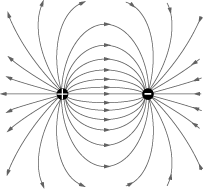
\includegraphics[width=0.9\textwidth]{EFeld}
	\caption{Feldlinien zwischen zwei geladenen Teilchen}
\end{figure}

Feldlinien\endnote{\glqq Camposcargas\grqq{} by http://commons.wikimedia.org/wiki/User:Chanchocan - Own work. Licensed under CC BY-SA 3.0 via Commons - \url{https://commons.wikimedia.org/wiki/File:Camposcargas.PNG}} sind ein Modell zur Verdeutlichung von grundlegenden Eigenschaften eines elektrischen Feldes. Sie schneiden sich nie und haben eine Richtung, die durch Pfeile angezeigt wird. Sollten sie von einem Körper ausgehen oder auf einen Körper auftreffen, stehen sie senkrecht auf dessen Oberfläche. Außerdem gibt die Dichte der Linien die Stärke des Feldes an.\endnote{Paragraph von: Armin Kunz: \glqq Bewertung der 1. Klausur\grqq{} vom 09.10.2014} Die Pfeile der Feldlinien zeigen immer zum negativen Pol.

Bei der Wechselwirkung zweier Körper gibt es eine abstoßende Kraftwirkung bei gegenläufigen Feldlinien und eine anziehende Kraftwirkung, wenn die Feldlinien in dieselbe Richtung zeigen.


\subsection{Coulomb'sches Gesetz} \label{subsec:CoulombGesetz}

Wenn nun klar ist, dass sich Ladungen beeinflussen, ist der nächste Schritt diesen \glqq Einfluss\grqq{} mathematisch auszudrücken. Dazu gibt es das Coulomb'sche Gesetz, welches die Kraft, die zwei kugelförmige (sphärische) Körper aufeinander auswirken, in Abhängigkeit von deren Ladungen und dem Abstand, angibt:

\begin{equation} \label{eq:coulomb_gesetz}
	F = \frac{1}{4\pi \cdot \epsilon_0} \cdot \frac{Q_1 \cdot Q_2}{d^{2}}
\end{equation}

Die Gleichung besteht aus einem konstanten Faktor, der die sogenannte \glqq Permittivität\grqq{} (\glqq elektrische Feldkonstante\grqq ) $\epsilon_0$ beinhaltet (\casio{32}), und einem variablen Teil der die Beträge der beiden Ladungen $Q_1$ und $Q_2$, und den Abstand der Mittelpunkte $d$ enthält.

Die Einheit Ladung ist $C$ (sprich: \glqq Coulomb\grqq ), was gleich $A \cdot s$ ist. Dies folgt daraus, dass Stromstärke als Ladung pro Zeit ($\frac{Q}{t}$) definiert ist; daher kann man Ladung als Stromstärke \emph{mal} Zeit ($A \cdot t$).

Eine Einheitenrechnung sieht dann wie folgt aus:

\begin{align}\label{eq:coulomb_gesetz_einheiten}
\begin{split}
	N 							&= \frac{1}{\epsilon_0} \cdot \frac{As \cdot As}{m^{2}} \\
	\frac{kg \cdot m}{s^{2}} 	&= \frac{1}{\epsilon_0} \cdot \frac{A^{2} \cdot s^{2}}{m^{2}}
\end{split}
\end{align}

\noindent Daraus ergibt sich als Einheit für die Feldkonstante $\epsilon_0$:

\begin{align}\label{eq:feldkonstante_einheiten}
\begin{split}
	\epsilon_0 &= \frac{A^{2} \cdot s^{2}}{m^{2}} \cdot \frac{s^{2}}{kg \cdot m} \\
	\epsilon_0 &= \frac{A^{2} \cdot s^{4}}{m^{3} \cdot kg} \\
	\epsilon_0 &= \frac{As}{Vm}
\end{split}
\end{align}

\begin{Aufgabe}
Versuche über die Definition des Volts ($V=\frac{kg \cdot m^2}{A \cdot s^3}$) von der vorletzten auf die letzte Umformung zu kommen! Einheitenrechnungen sind wichtig!
\end{Aufgabe}

\begin{NiceToKnow}
Diese Form der Gleichung ist analog zu Newtons Gravitationsgesetz: $F = G \cdot \frac{m_1 \cdot m_2}{d^2}$. Hierbei ist $G$ ebenfalls eine Konstante, nämlich die Gravitätskonstante.
\end{NiceToKnow}


\subsection{Homogenes Feld} \label{subsec:EFeldHomogen}

Das elektrische Feld zwischen zwei geladenen Körpern ist meistens inhomogen. Das heißt, dass die Feldstärke, also die Dichte der Feldlinien nicht überall gleich ist. Für Berechnungen würde dies das Lösen von komplexen Differentialgleichungen voraussetzen. Daher wird in der Schulphysik fast immer von einem homogenen Feld ausgegangen, wenn Berechnungen an einem elektrischen Feld anstehen:

\begin{itemize}
	\item Die Feldlinien sind alle parallel.
	\item Die Feldlinien zeigen alle in dieselbe Richtung.
	\item Die Feldlinien haben alle denselben Abstand zueinander.
\end{itemize} 

\noindent Eine Möglichkeit, so ein Feld zu generieren, ist der Plattenkondensator (\referenz{sec:plattenkondensator}).


\subsection{Feldstärke}  \label{subsec:Feldstaerke}

In einem homogenen Feld ist die Feldstärke (Formelzeichen: $E$) also an jedem Punkt gleich. Sie ordnet jedem geladenen Körper eine Kraft und, würde man mit Vektoren rechnen, eine Richtung zu:

\begin{equation} \label{eq:feldstaerke}
	\vec{E} = \frac{\vec{F}}{q}
\end{equation}

\noindent $q$ ist hierbei die \emph{vorzeichenbehaftete} Ladung des Probekörpers im Feld. Als Einheit ergibt sich $\frac{N}{C}$ für die Feldstärke $E$. 

Umgeformt für $F$ ergibt sich aus der Gleichung:

\begin{equation} \label{eq:feldstaerke_nach_F}
	\vec{F} = q \cdot \vec{E}
\end{equation}











\section{Phänomene}

%%%%% TITLE OF MAIN DOCUMENT %%%%%
%% NUMBER AND TITLE OF SECTION %%


%Some sample text to be displayed above the first subsection

%\subsection{Prinzip}

%Ein Zyklotron besteht aus Zwei hohlen, halbzylindrischen und Duanden an denen eine Spannung mit unterschiedlichem Vorzeichen anliegt, und darüber bzw. darunter liegende Magneten, die ein homogenes Magnetfeld erzeugen. Zudem gibt es einen Einlass und einen Auslass für Teilchen.

%\begin{wrapfigure}{r}{0.4\textwidth} \label{Zyklo}
%
%	\vspace{-10pt}
%	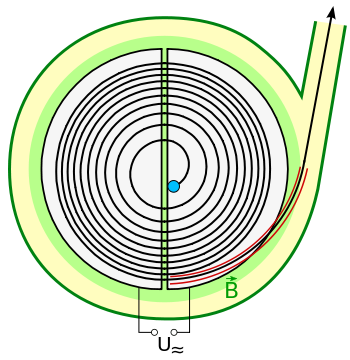
\includegraphics[width=0.35\textwidth]{Zyklotron_Prinzipskizze02.png}
%	\vspace{-13pt}
%	\caption{Prinzipskizze eines Zyklotrons}
%	\vspace{-5pt}	
%	
%\end{wrapfigure}

%\subsubsection{Anwendung}

% Some Formula:

%\begin{equation}
%	x= \frac{y \cdot 13 \pi z}
%			{\cos \alpha}
%\end{equation}

%%%%%%%%%%%%%%%%%%%%%%%
% Eigentlicher Beginn %
%%%%%%%%%%%%%%%%%%%%%%%

\subsection{Abschirmung}

\begin{figure}[!h]
	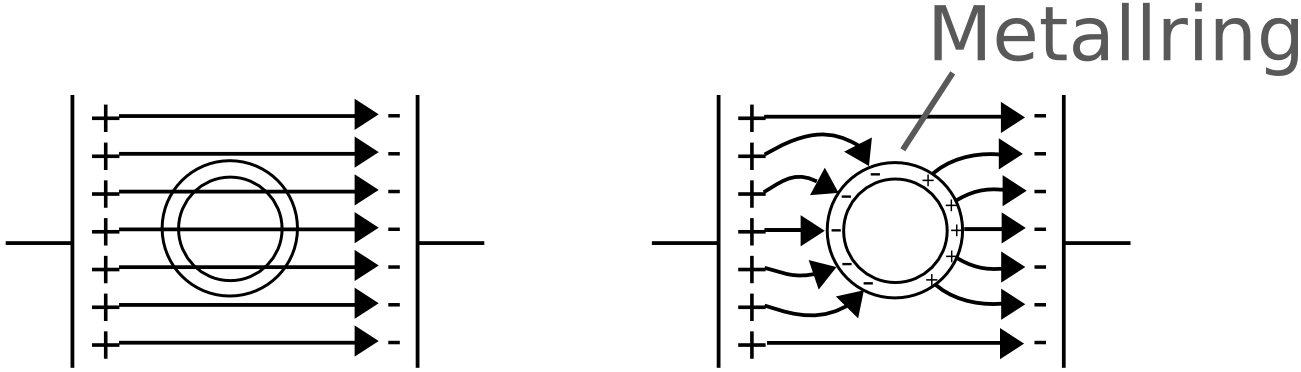
\includegraphics[width=\textwidth]{Abschirmung}
	\caption{Abschirmung eines elektischen Feldes durch einen Metallring}
	\label{fig:abschrimung}
\end{figure}

In einem zweidimensionalen elektrischen Feld kann durch einen geschlossenen Ring aus Metall ein elektrischen Feld abgeschirmt werden. Dies passiert, da die beweglichen negativen Ladungen im Metallring zur positiven Seite des äußeren Feldes wandern (entgegen der Feldlinien) und auf der anderen Seite des Ringes ein positive Ladung hinterlassen. Diese Ladungstrennung führt ihrerseits zum Aufbau eines elektrischen Feldes, welches in die entgegengesetzte Richtung zeigt und das \glqq äußere\grqq{} Feld im Inneren des Rings neutralisiert.\endnote{Abbildung von: \url{http://www.schule.promathika.de/uploads/PhysikSkript/Faraday_Becher.jpg}}

Im dreidimensionalen Raum ist dafür eine Hülle nötig, die man dann \glqq Faradayischer Käfig\grqq{} nennt.


\section{Plattenkondensator} \label{sec:plattenkondensator}

%%%%% Elektrisches Feld %%%%%
%% #3 Kondensator %%


%Some sample text to be displayed above the first subsection

%\subsection{Prinzip}

%Ein Zyklotron besteht aus Zwei hohlen, halbzylindrischen und Duanden an denen eine Spannung mit unterschiedlichem Vorzeichen anliegt, und darüber bzw. darunter liegende Magneten, die ein homogenes Magnetfeld erzeugen. Zudem gibt es einen Einlass und einen Auslass für Teilchen.

%\begin{wrapfigure}{r}{0.4\textwidth} \label{Zyklo}
%
%	\vspace{-10pt}
%	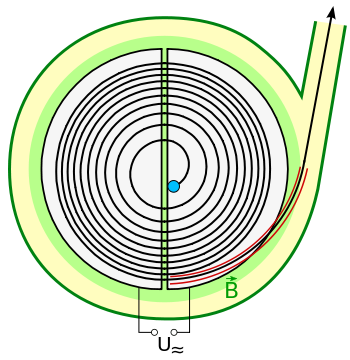
\includegraphics[width=0.35\textwidth]{Zyklotron_Prinzipskizze02.png}
%	\vspace{-13pt}
%	\caption{Prinzipskizze eines Zyklotrons}
%	\vspace{-5pt}	
%	
%\end{wrapfigure}

%\subsubsection{Anwendung}

% Some Formula:

%\begin{equation}
%	x= \frac{y \cdot 13 \pi z}
%			{\cos \alpha}
%\end{equation}

%%%%%%%%%%%%%%%%%%%%%%%
% Eigentlicher Beginn %
%%%%%%%%%%%%%%%%%%%%%%%

Der Plattenkondensator (im Folgenden nur noch Kondensator genannt) ist ein wichtiges Element der Elektrotechnik. Auch eignet er sich seht gut, um in der Schulphysik verschiedene Aspekte von elektrischen Feldern zu zeigen.


\subsection{Definition} \label{subsec:kon_def}

\begin{figure}[h!]
	\centering
	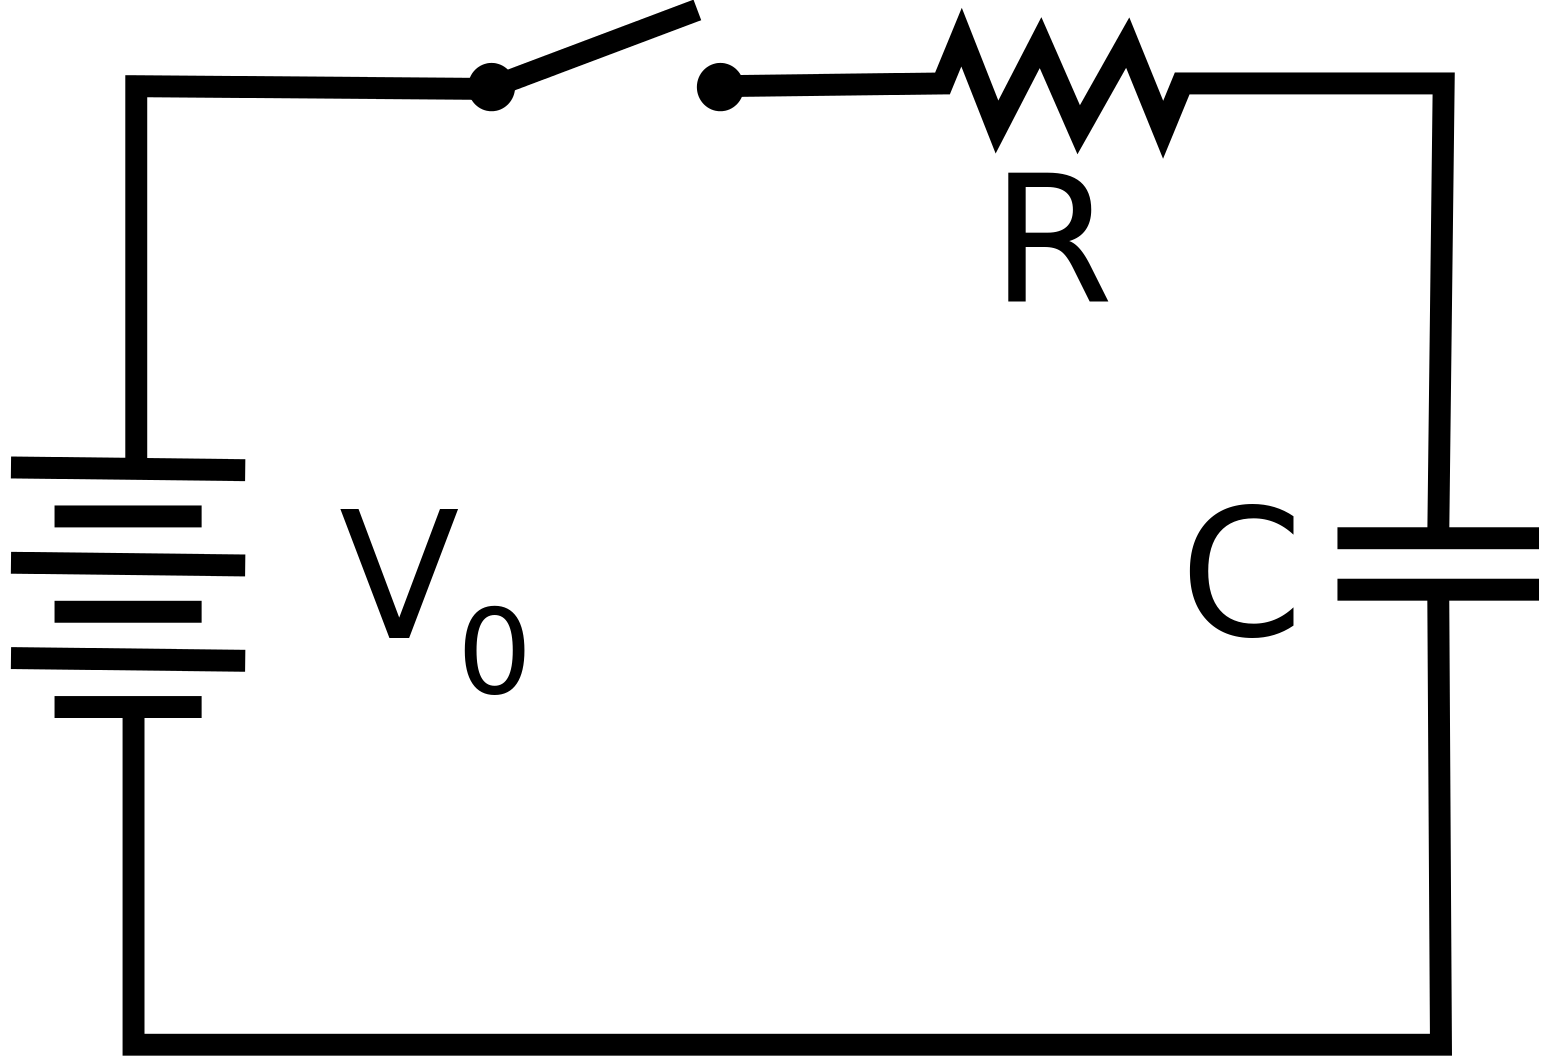
\includegraphics[width=0.6\textwidth]{RCWiring}
	\caption{Ein Schaltkreis mit Kondensator $C$ und Widerstand $R$}
	\label{fig:CapWiring}
\end{figure}

Ein Plattenkondensator besteht aus zwei ungleichnamig geladenen Platten, die sich parallel gegenüberstehen. Sie sind an ein Spannungsquelle angeschlossen. In einem Schaltplan wird er wie in Abbildung \ref{fig:CapWiring} \footnote{"RC switch" by PureCore - Own work. Licensed under CC BY-SA 3.0 via Commons - \url{https://commons.wikimedia.org/wiki/File:RC_switch.svg}} notiert.

\begin{Wichtig}
An sich fließt kein Strom durch den Kondensator! Die Platten sind elektrisch getrennt; das Dielektrikum, also das nicht-leitende Material zwischen den Platten (z.B. Luft), isoliert. 
\end{Wichtig}


\subsection{Elektrisches Feld im Inneren des Kondensators}

\begin{figure}[h!]
	\centering
	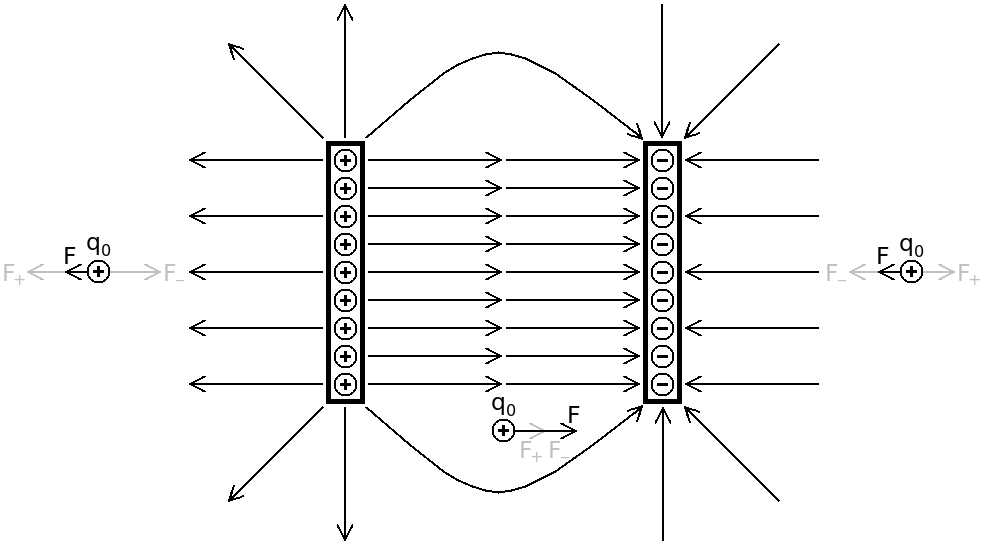
\includegraphics[width=\textwidth]{EFeldKondensator}
	\caption{Das elektrische Feld in und um einen Plattenkondensator}
\end{figure}

Durch den Überschuss positiver Ladungen auf der einen Seite und negativer Ladungen auf der Anderen, ergibt sich ein homogenes Magnetfeld zwischen den Platten.\footnote{„E Feld Kondensator“. Über Wikibooks - \url{https://de.wikibooks.org/wiki/Datei:E_Feld_Kondensator.png}}

\subsubsection{Feldstärke}

Die Stärke des Feldes im Inneren lässt sich auf recht einfach Art aus der anliegenden Spannung $U$ und dem Plattenabstand $d$ berechnen:

\begin{equation} \label{eq:feldstaerke_kondensator}
	E = \frac{U}{d}
\end{equation}

Die resultierende Einheit $\frac{V}{m}$ ist äquivalent zu $\frac{N}{C}$, der generellen Einheit für die Feldstärke (Siehe \referenz{subsec:Feldstaerke}).

\begin{Aufgabe}
Zeige, dass $\frac{V}{m}$ äquivalent zu $\frac{N}{C}$ ist, indem Du die Definitionen der Einheiten Volt $V=\frac{kg \cdot m^2}{A \cdot s^3}$, Newton und Coulomb einsetzt.

Einheitenrechnungen sind praktisch, um Ansätze für Herleitungen zu verifizieren. Am Ende muss auch immer die richtige Einheit für eine Größe aus den Größen in der Formel herauskommen.

Der Leser fühle sich hiermit eingeladen, eine Einheitenrechnung für jede hier aufgeführte Gleichung anzustellen. 
\end{Aufgabe}

\subsubsection{Kraft auf Körper}

In die allgemeine Gleichung für eine Kraft auf einen geladenen Körpern (Gleichung \ref{eq:feldstaerke_nach_F} auf Seite \pageref{eq:feldstaerke_nach_F}: $\vec{F} = q \cdot \vec{E}$) kann nun die obige Gleichung für $E$ im Kondensator eingesetzt werden (Gleichung \ref{eq:feldstaerke_kondensator}):

\begin{equation} \label{eq:kraft_kondensator}
	F = q \cdot \frac{U}{d}
\end{equation}

In diesem Fall kann sowieso auf eine Vektorrechnung verzichtet werden, da die Richtung der des elektrischen Felds klar und das Feld homogen ist.

\subsubsection{Energieumsatz bei einer Bewegung eines Körpers}

Wenn ein Körper in einem Kondensator bewegt wird, wird dabei Energie umgesetzt. Eine äquivalente Ausdrucksweise wäre, es wird \glqq Arbeit verrichtet\grqq . Das geschieht gemäß dieser Formel, bei der $s$ die Strecke ist, um die der Körper verschoben wird:

\begin{equation} \label{eq:arbeit}
	W = F \cdot s
\end{equation}

\noindent Die Kraft $F$ kann durch Umstellen mit $F = q \cdot E$ zu

\begin{equation} \label{eq:arbeit_kondensator}
	W = q \cdot E \cdot s
\end{equation}

\noindent ersetzt werden.

\begin{NiceToKnow}
$W = q \cdot E \cdot s$ ist analog zur Lagearbeit aus der Mechanik: $W_{pot} = m \cdot g \cdot h$
\end{NiceToKnow}


\subsection{Flächenladungsdichte}

Die elektrische Feldstärke im Inneren eines Kondensators lässt sich auch über die Flächenladungsdichte berechnen. Die Flächenladungsdichte $\sigma$ (Spricht: \glqq klein Sigma\grqq ) gibt an, wie \emph{dicht} Ladungen auf den Kondensatorplatten verteilt sind:

\begin{equation} \label{eq:flaechenladungsdichte}
	\sigma = \frac{Q}{A}
\end{equation}

\begin{NiceToKnow}
Man schreibt $q$ für eine spezifische, unveränderbare Ladung eines Probekörpers und $Q$ für z.B. die Ladung von Kondensatorplatten oder den Betrag eines Ladungsflusses durch einen Leiter.
\end{NiceToKnow}

Die Flächenladungsdichte ist im homogenen Feld proportional zur Feldstärke ($\sigma \sim E$). Die Proportionalitätskonstante hierbei ist $\frac{1}{\epsilon_0}$ (Siehe \referenz{subsec:CoulombGesetz}), sodass sich ergibt:

\begin{equation} \label{eq:feldstaerke_mit_sigma}
	E = \frac{\sigma}{\epsilon_0} = \frac{1}{\epsilon_0} \cdot \frac{Q}{A}
\end{equation}

\subsubsection{Exkurs: Flächenladungsdichte bei Kugeln}

Die Oberfläche von Kugeln ist als $A=4\pi \cdot r^2$ definiert. Daher ergibt sich ein Spezialfall für die Feldstärke:

\begin{equation} \label{eq:feldstaerke_kugel}
	E = \frac{1}{\epsilon_0} \cdot \frac{Q}{4\pi \cdot r^2} = \frac{1}{4\pi \cdot \epsilon_0} \cdot \frac{Q}{r^2}
\end{equation}

Es fällt eine Ähnlichkeit mit dem Coulomb-Gesetz (Gleichung \gleichungsreferenz{eq:coulomb_gesetz}) auf, welches die Kraft zwischen zwei geladenen, sphärischen Körpern angibt.


\subsection{Kapazität des Kondensators}

Die wichtigste elektrische Größe eines Kondensators ist die Kapazität $C$ mit Einheit \glqq Farad\grqq{}, Zeichen $F = \frac{A \cdot s}{V} = \frac{A^2 \cdot s^4}{kg \cdot m^2} = \frac{A^2 \cdot s^2}{N \cdot m}$:

\begin{equation} \label{eq:kapazitaet}
	C = \frac{Q}{U}
\end{equation}

Die Kapazität gibt also an, wie viel Ladung ein Kondensator bei einer definierten Spannung fasst, bzw. wie hoch die Spannung sein muss, damit die definierte Ladung $Q$ auf den Kondensator \glqq geht\grqq .

Für eine Bestimmungsgleichung, welche nur aus Kenngrößen besteht, muss $Q$ ersetzt werden. Mit den beiden Definitionen für die Feldstärke ($E = \frac{\sigma}{\epsilon_0}$ und $E=\frac{U}{d}$) ergibt sich für $Q$:

\begin{align}
\begin{split}
	E = \frac{\sigma}{\epsilon_0} \\
	E = \frac{Q}{A \cdot \epsilon_0} \\
	\frac{U}{d} = \frac{Q}{A \cdot \epsilon_0} \\
	Q = \epsilon_0 \cdot \frac{U \cdot A}{d}
\end{split}
\end{align}

\noindent Dieses $Q$ lässt sich in die Gleichung für $C$ einsetzen:

\begin{equation}
	C = \epsilon_0 \cdot \frac{U \cdot A}{d \cdot U} = \epsilon_0 \epsilon_r \cdot \frac{A}{d}
\end{equation}

Die Spannung $U$ kürzt sich und es wurde ein weitere Konstante $\epsilon_r$ eingeführt. Die \glqq relative Feldkonstante\grqq{} charakterisiert die verstärkenden oder schwächenden Eigenschaften des Dielektrikum (\referenz{subsec:kon_def}). Für Luft bzw. Vakuum ist sie $\approx 1$. Es gibt jedoch Materialien, die durch eine hohe relative Feldkonstante die Kapazität um Faktoren bis ca. $10^3$ erhöhen.

\begin{NiceToKnow}
$BaTiO_3$, Bariumthiooxid, hat eine $\epsilon_r$ von $10^2-10^3$\footnote{Aus: \url{http://www.techniklexikon.net/d/dielektrizitaetskonstante/dielektrizitaetskonstante.htm}}
\end{NiceToKnow}


\subsection{Verschaltung von Kondensatoren}

\subsubsection{Parallel}

\begin{figure}[h!]
	\centering
	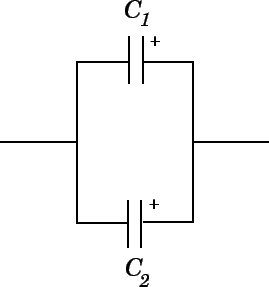
\includegraphics[width=0.5\textwidth]{CapsParallel}
	\caption{Parallelschaltung zweier Kapazitäten (= Kondensatoren) $C_1$ und $C_2$}
\end{figure}

Wenn Kondensatoren in einem Stromkreis parallel\footnote{Abbildung von: \url{http://farside.ph.utexas.edu/teaching/302l/lectures/node46.html}} geschaltet werden, addieren sich die Kapazitäten. Man kann sagen, dass die effektive Platte größer wird und daher mehr Ladung pro Spannung tragen kann (Siehe \gleichungsreferenz{eq:kapazitaet}):

\begin{equation}
	C_{ges} = \sum\limits_{i=1}^n C_i = C_1 + C_2 + \cdots + C_n
\end{equation}

\noindent Die Spannung bleibt dann aufgrund derselben Beziehung an jedem Element konstant:

\begin{equation}
	U_{ges} = U_1 = U_2 = \cdots = U_n
\end{equation}


\subsubsection{In Reihe}

\begin{figure}[h!]
	\centering
	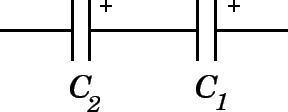
\includegraphics[width=0.5\textwidth]{CapsSeries}
	\caption{Reihenschaltung zweier Kapazitäten (= Kondensatoren) $C_1$ und $C_2$}
\end{figure}

Wenn Kondensatoren in einem Stromkreis in Reihe\footnote{Abbildung von: \url{http://farside.ph.utexas.edu/teaching/302l/lectures/node46.html}} geschaltet werden, ist die Summe der Kehrwerte der einzelnen Kapazitäten der Kehrwert der Gesamtkapazität. Das liegt daran, dass das \glqq Mittelstück\grqq , also die positive Plattes von $C_1$ und die negative Platte von $C_2$, ein definierte Ladung tragen, das heißt die positiven und negativen Ladungen können nur durch Influenz (Siehe \referenz{subsec:Influenz}) auftreten, da dieses Stück elektrisch vom Rest des Schaltkreises, also auch von einer mögliches Ladungsquelle getrennt ist.

Daher ist die Gesamtkapazität der Schaltung $0F$, wenn einer der beiden Kondensatoren die Kapazität $0F$ hat; $0,5F$, wenn beide Kondensatoren die Kapazität $1F$ haben; und die Gesamtkapazität kann nie größer sein als die niedrigste Einzelkapazität in der Kondensatorschaltung.

\begin{equation}
	\frac{1}{C_{ges}} = \sum\limits_{i=1}^n \frac{1}{C_i} = \frac{1}{C_1} + \frac{1}{C_2} + \cdots + \frac{1}{C_n}
\end{equation}

\noindent Wie auch bei der Reihenschaltung von Widerständen oder Spannungsquellen, addieren sich die Spannungen an den einzelnen Elementen zur Gesamtspannung:

\begin{equation}
	U_{ges} = \sum\limits_{i=1}^n U_i = U_1 + U_2 + \cdots + U_n
\end{equation}




\section{Elektronenbewegung im Elektrischen Feld}

%%%%% TITLE OF MAIN DOCUMENT %%%%%
%% NUMBER AND TITLE OF SECTION %%


%Some sample text to be displayed above the first subsection

%\subsection{Prinzip}

%Ein Zyklotron besteht aus Zwei hohlen, halbzylindrischen und Duanden an denen eine Spannung mit unterschiedlichem Vorzeichen anliegt, und darüber bzw. darunter liegende Magneten, die ein homogenes Magnetfeld erzeugen. Zudem gibt es einen Einlass und einen Auslass für Teilchen.

%\begin{wrapfigure}{r}{0.4\textwidth} \label{Zyklo}
%
%	\vspace{-10pt}
%	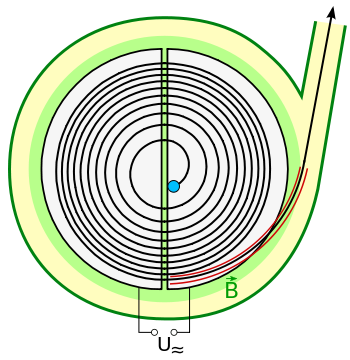
\includegraphics[width=0.35\textwidth]{Zyklotron_Prinzipskizze02.png}
%	\vspace{-13pt}
%	\caption{Prinzipskizze eines Zyklotrons}
%	\vspace{-5pt}	
%	
%\end{wrapfigure}

%\subsubsection{Anwendung}

% Some Formula:

%\begin{equation}
%	x= \frac{y \cdot 13 \pi z}
%			{\cos \alpha}
%\end{equation}

%%%%%%%%%%%%%%%%%%%%%%%
% Eigentlicher Beginn %
%%%%%%%%%%%%%%%%%%%%%%%


Da Elektronen negativ geladen sind (es \emph{sind} negative Ladungen), werden sie im elektrischen Feld zur positiven Seite hin beschleunigt, das heißt entgegen der Feldlinien. 

\subsection{Einwirkende Kraft}

Die Kraft ist abhängig von der Feldstärke und der Elektronenladung:

\begin{equation}
	F_{el} = E \cdot q_e
\end{equation}

\noindent Die Elektronenladung $q_e$ ist die konstante Ladung \emph{eines} Elektrons (\casio{23}). Zur experimentellen Bestimmung dieser, siehe \referenz{sec:Millikan}.

Im Kondensator gilt dann mit $E=\frac{U}{d}$:

\begin{equation} \label{eq:F_el}
	F_{el} = \frac{U}{d} \cdot q_e
\end{equation}



\section{Bewegungsgesetze für Elektronen} \label{sec:BewegungsgesetzElektronen}

%%%%% Elektrisches Feld %%%%%
%% #4 Elektronenbewegung im Elektrischen Feld %%


%Some sample text to be displayed above the first subsection

%\subsection{Prinzip}

%Ein Zyklotron besteht aus Zwei hohlen, halbzylindrischen und Duanden an denen eine Spannung mit unterschiedlichem Vorzeichen anliegt, und darüber bzw. darunter liegende Magneten, die ein homogenes Magnetfeld erzeugen. Zudem gibt es einen Einlass und einen Auslass für Teilchen.

%\begin{wrapfigure}{r}{0.4\textwidth} \label{Zyklo}
%
%	\vspace{-10pt}
%	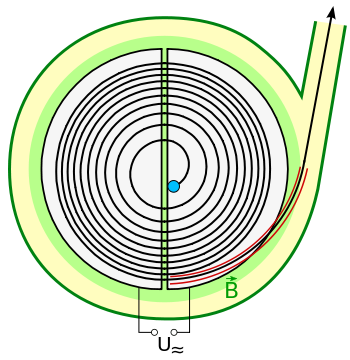
\includegraphics[width=0.35\textwidth]{Zyklotron_Prinzipskizze02.png}
%	\vspace{-13pt}
%	\caption{Prinzipskizze eines Zyklotrons}
%	\vspace{-5pt}	
%	
%\end{wrapfigure}

%\subsubsection{Anwendung}

% Some Formula:

%\begin{equation}
%	x= \frac{y \cdot 13 \pi z}
%			{\cos \alpha}
%\end{equation}

%%%%%%%%%%%%%%%%%%%%%%%
% Eigentlicher Beginn %
%%%%%%%%%%%%%%%%%%%%%%%


\begin{Wichtig}
Diese Bewegungsgesetze und Bewegungsgesetze allgemein sind wiederkehrendes Grundmaterial in der Schulphysik und sollten daher \glqq aus dem FF\grqq{} beherrscht werden. Siehe: \ref{sec:bewegungsgesetze}.
\end{Wichtig}

\subsection{Bewegung parallel zu den Feldlinien} \label{subsec:BewegungsgesetzParallel}

Auf ruhende Elektronen, oder Elektronen, die sich parallel zu den Feldlinien des elektrischen Feldes bewegen, wirkt eine Kraft, welche sie ebenfalls parallel zu den Feldlinien beschleunigt. Daher ist und bleibt diese Bewegung eindimensional und sie lässt sich durch \emph{ein} Weg-Zeit Gesetz der gleichmäßig beschleunigten Bewegung ausdrücken (vgl. vertikaler Wurf):

%%%%%%%%%%%%%%%%%%%%%
% WEG ZEIT GESETZE %%
%%%%%%%%%%%%%%%%%%%%%

Nach Newton gilt $F = m \cdot a$, was sich zu $a = \frac{F}{m}$ umstellen lässt. $F_{el}$ (Siehe: \gleichungsreferenz{eq:F_el}) lässt sich nun für $F$ einsetzten und die Elektronenmasse $m_e$, welche konstant ist (\casio{03}), für $m$:

\begin{equation}
	a = \frac{q_e \cdot E}{m_e}
\end{equation}


Folgendes Weg-Zeit-Gesetz für den Weg der Feldlinien entgegen, lässt sich aufstellen:

\begin{align} \label{eq:s(t)Allgemein}
\begin{split}
	s(t) &= \frac{1}{2} a \cdot t^2 + v_0 \cdot t + s_0 \\
	s(t) &= \frac{q_e \cdot E}{2m_e} \cdot t^2 + v_0 \cdot t + s_0
\end{split}
\end{align}

\noindent In diesem Fall steht $v_0$ für die angesprochene mögliche Anfangsgeschwindigkeit, die das Elektron bereits \glqq drauf hatte\grqq{} und $s_0$ für eine mögliche Anfangsstrecke, die das Elektron vor Beeinflussung durch das elektrische Feld schon zurückgelegt hatte.

\begin{Wichtig}
Beim Einsetzen von $v_0$ auf das Vorzeichen achten! Z.B. muss eine Geschwindigkeit, die der Beschleunigungsrichtung  entgegengesetzt ist, also in Richtung der Feldlinien verläuft, mit negativem Vorzeichen notiert werden.
\end{Wichtig}

Dieses Gesetz kann spezifischer für die Bewegung in einem Plattenkondensator mit eingesetztem $E=\frac{U}{d}$ (Siehe \gleichungsreferenz{eq:feldstaerke_kondensator}) ausgedrückt werden:

\begin{align} \label{eq:s(t)imKondensator}
\begin{split}
	s(t) = \frac{q_e \cdot U}{2d \cdot m_e} \cdot t^2 + v_0 \cdot t + s_0
\end{split}
\end{align}


\subsection{Bewegung senkrecht zu den Feldlinien} \label{subsec:BewegungsgesetzSenkrecht}

Etwas komplexer wird es, wenn sich ein Elektron senkrecht zu den Feldlinien eines elektrischen Feldes bewegt. Analog zu den Berechnungen eines horizontalen Wurfs (z.B. Abwurf von Ladung von einem Flugzeug) muss auch hier die Bewegung in eine horizontale Bewegung (\glqq in x-Richtung\grqq) und eine vertikale Bewegung (\glqq in y-Richtung\grqq) aufgeteilt werden. 

Die Bewegung in x-Richtung ist als einfache gleichförmige Bewegung nach $x(t)=v \cdot t + x_0$ zu beschreiben. 

Die Bewegung in y-Richtung kann aus Gleichung \ref{eq:s(t)Allgemein} oder \ref{eq:s(t)imKondensator} übernommen werden.

Um beide Bewegungen in einer einzigen Gleichung zusammenzufassen, also den y-Weg in Abhängigkeit der x-Position anzugeben und damit die Position des Elektrons eindeutig zu bestimmen, muss $x(t)$ nach $t$ umgestellt werden und dieses $t$ in die Gleichung von $s(t)$ eingesetzt werden. 

\begin{NiceToKnow}
Zur Vereinfachung wird in den allermeisten Aufgaben zu diesem Thema auf einen Anfangswert, also auf $v_0$, $y_0$ o.ä. verzichtet. So auch in dieser Herleitung.
\end{NiceToKnow}

Zudem wird die Funktion für den Weg in y-Richtung nicht mehr $s(t)$, sondern $y(t)$ genannt, um sie besser von $x(t)$ abzugrenzen.

\begin{align} \label{eq:x(t)Senkrecht}
\begin{split}
	x(t) &= v_x \cdot t \\
	t(x) &= \frac{x}{v}
\end{split}
\end{align}

\noindent Es folgt das Einsetzten in die allgemeine Form von $y(t)$ (Siehe: \gleichungsreferenz{eq:s(t)Allgemein}):

\begin{align} \label{eq:y(x)Allgemein}
\begin{split}
	y(t) &= \frac{q_e \cdot E}{2m_e} \cdot t^2 \\
	y(x) &= \frac{q_e \cdot E}{2m_e} \cdot \frac{x^2}{v_{x}^2}
\end{split}
\end{align}

\noindent Spezifisch in einem Kondensator:

\begin{align} \label{eq:y(x)imKondensator}
\begin{split}
	y(t) &= \frac{q_e \cdot U}{2d \cdot m_e} \cdot t^2 \\
	y(x) &= \frac{q_e \cdot U}{2d \cdot m_e} \cdot \frac{x^2}{v_{x}^2}
\end{split}
\end{align}








\section{Millikanversuch} \label{sec:Millikan}

%%%%% Elektrisches Feld %%%%%
%% Millikanversuch %%


%Some sample text to be displayed above the first subsection

%\subsection{Prinzip}

%Ein Zyklotron besteht aus Zwei hohlen, halbzylindrischen und Duanden an denen eine Spannung mit unterschiedlichem Vorzeichen anliegt, und darüber bzw. darunter liegende Magneten, die ein homogenes Magnetfeld erzeugen. Zudem gibt es einen Einlass und einen Auslass für Teilchen.

%\begin{wrapfigure}{r}{0.4\textwidth} \label{Zyklo}
%
%	\vspace{-10pt}
%	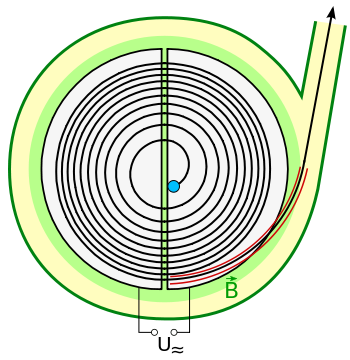
\includegraphics[width=0.35\textwidth]{Zyklotron_Prinzipskizze02.png}
%	\vspace{-13pt}
%	\caption{Prinzipskizze eines Zyklotrons}
%	\vspace{-5pt}	
%	
%\end{wrapfigure}

%\subsubsection{Anwendung}

% Some Formula:

%\begin{equation}
%	x= \frac{y \cdot 13 \pi z}
%			{\cos \alpha}
%\end{equation}

%%%%%%%%%%%%%%%%%%%%%%%
% Eigentlicher Beginn %
%%%%%%%%%%%%%%%%%%%%%%%


Der Millikanversuch war ein Experiment des amerikanischen Physikers Robert Millikan von 1910, dessen Ergebnisse ihm 1923 den Nobelpreis einbrachte. Mit diesem Versuch konnte die Existenz einer kleinsten Elementarladung nachgewiesen werden und diese Elektronenladung recht genau bestimmt werden.

\subsection{Vorgehensweise}

Millikans Ansatz war recht simpel. Er zerstäubte flüssiges Öl mit einer Pumpe so, dass die Tropfen extrem klein und durch Reibung mit der Pumpendüse negativ geladen wurden. Diese wurden in einen Plattenkondensator geleitet und mit einem Mikroskop deren Bahn beobachtet. Mittels Einstellen der Spannung am horizontal zur Erdoberfläche ausgerichteten Kondensator wurde ein Tröpfchen zum Schweben gebracht, indem das elektrische Feld entgegen der Fallbeschleunigung der Erde wirkte.

Damit ergab sich der Ansatz, die elektrische Kraft $F_{el}=q \cdot E$ (\gleichungsreferenz{eq:feldstaerke_nach_F}) gleich der Gewichtskraft $F_G = m \cdot q$ zu setzten. Wie schon so oft kann dann für $E$ die homogene Feldstärke im Kondensator eingesetzt werden: $E = \frac{U}{d}$:

\begin{align} \label{eq:MillikanAnsatz}
\begin{split}
	F_{el} &= F_G \\
	q \cdot E &= m \cdot g \\
	q &= \frac{m \cdot g}{E} \\
	q &= \frac{m \cdot g \cdot d}{U}
\end{split}
\end{align}


\subsection{Umgehung der direkten Massebestimmung}

Bis auf die Masse sind in der obigen Gleichung alle Größen gegeben bzw. messbar. Das bestimmen der Masse stellte allerdings ein Problem dar, da die Tröpfchen viel zu klein waren um ihre Masse auf klassische Art zu bestimmen (z.B. wiegen). Auch die Bestimmung über das Volumen und die Dichte des Öls erwiesen sich als unpraktisch, da der Durchmesser eines Tröpfchens aufgrund von optischen Eigenschaften der Mikroskoplinsen nur sehr unpräzise gemessen werden konnte.

Daher hat sich Robert Millikan dem Gesetz von Stokes\footnote{Gesetz von Stokes: \url{https://de.wikipedia.org/wiki/Gesetz_von_Stokes}} zur Reibung von spährischen (\glqq kugelförmigen\grqq) Körpern in Gasen oder Flüssigkeiten bedient: 

Mit dem Gesetz lässt sich der Radius eines Öltröpfchens über dessen Fallgeschwindigkeit berechnen, welche im selben Experiment bestimmt werden kann: Durch Abschalten der Kondensatorspannung und Stoppen der Zeit, die der Tropfen für das Zurücklegen einer bestimmten Strecke benötigte, die in Form eines Rasters auf dem Mikroskop erkennbar war, konnte die Fallgeschwindigkeit berechnet werden. Zudem war diese Geschwindigkeit nach einer kurzen Beschleunigungsphase durch die Luftreibung konstant.

Die Stokesreibung ist im Schwebefall gleich der Differenz aus Gewichtskraft und Auftrieb des Tröpfchens: $F_R = F_G - F_A$. Setzt man die entsprechenden Teilgleichungen (Gewichtskraft einer Kugel $F_G = V \rho g = \frac{4}{3} \pi r^3 \rho_{O} g$ und Auftrieb einer Kugel in der Luft $F_A = V \rho g = \frac{4}{3} \pi r^3 \rho_L g$) ein, erhält man für $r$:

\begin{align} \label{eq:StokesReibungFuerR}
\begin{split}
	F_R &= F_G - F_A \\
	6 \pi \eta v_O r &= \frac{4}{3} r^3 \pi \rho_{O} g - \frac{4}{3} r^3 \pi \rho_{L} g \\
	r &= \sqrt{\frac{9v_{O}\eta}{2(\rho_{O}-\rho_{L}) \cdot g}}
\end{split}
\end{align}

Hierbei ist $v_{0}$ besagte Fallgeschwindigkeit, $\eta$ (spricht: \glqq klein Eta\grqq) die Viskosität der Luft, $\rho$ (sprich: \glqq klein Rho\grqq) jeweils die Dichte des Öls ($\rho_O$), respektive von Luft ($\rho_L$) und $g$ die Fallbeschleunigung.

Nun muss $F_{el}$ nicht gleich $F_{G}$ gesetzt werden, sondern gleich der Differenz $F_{G} - F_{A}$ um den Auftrieb in der Luft, welcher klein, aber bei dieser Größenordnung nicht zu vernachlässigen ist, mit einzubeziehen:

\begin{align}
\begin{split}
	F_{el} &= F_G - F_A \\
	\frac{qU}{d} &= \frac{4}{3} \pi r^3 \rho_{O} g - \frac{4}{3} \pi r^3\rho_{L} g \\
	\frac{qU}{d} &= \frac{4}{3} \pi  r^3(\rho_{O} - \rho_{L}) g \\
	q &= \frac{d}{U} \cdot \frac{4}{3} \pi r^3 (\rho_{O} - \rho_{L}) g \\
\end{split}
\end{align}

\noindent Jetzt noch $r$ von der Stokesreibung einsetzten:

\begin{align}
\begin{split}
	q &= \frac{d}{U} \cdot \frac{4}{3} \pi \sqrt{\frac{9v_{O}\eta}{2(\rho_{O}-\rho_{L}) \cdot g}}^3 (\rho_{O} - \rho_{L}) g \\
	q &= \frac{d}{U} \cdot 9\sqrt{2} \pi \cdot \sqrt{\frac{v_{O}^3 \cdot \eta^3}{(\rho_O - \rho_L) \cdot g}}
\end{split}
\end{align}

Damit existiert eine Gleichung für die Ladung $q$ eines Öltröpfchen, die nur aus messbaren Größen besteht.

\begin{Anmerkung}
Natürlich kann und muss die Herleitung als Schüler nicht komplett nachvollzogen werden. Wichtig sind ist der Ansatz und das Auftreten des Masseproblems. Wie genau dieses gelöst würde, ist nicht von unabdingbarer Bedeutung. Das Curriculum legt den Fokus mehr auf die richtige Interpretation der Ergebnisse; beschrieben im nächsten Abschnitt.
\end{Anmerkung}


\subsection{Ergebnisse}

\begin{figure}[h!]
	\center
	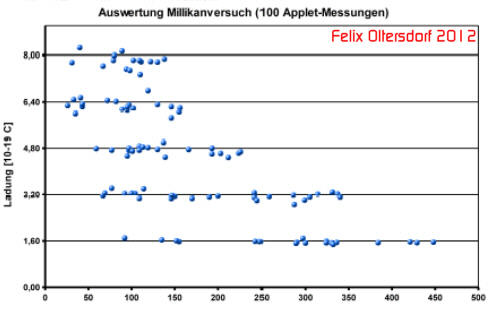
\includegraphics[width=0.7\textwidth]{millikan_auswertung}
	\caption{Auswertung via Graph: Ladung über Nummer der Durchführung}
	\vspace*{-10pt}
	\label{fig:millikan_auswertung}
\end{figure}

Wenn man die Ergebnisse wie in Grafik \ref{fig:millikan_auswertung} \footnote{Abbildung von: \url{http://physik-am-gymnasium.de/SekII/Elektrisches_Feld/millikan_auswertung.html}} aufführt, fällt auf, dass sich eine sogenannte Quantisierung einstellt. Das heißt, dass die Ladung nicht \glqq Stufenlos\grqq{} sondern in \glqq Sprüngen\grqq{} existiert. Mathematisch heißt das, dass die Ladungen der Tröpfchen Vielfache einer kleinsten Einheit sind, Vielfache der \glqq Elementarladung\grqq .

Diese Elementarladung (in Coulomb $C$) mit Formelzeichen $q_e$ oder $e$ (seltener auch einfach $q$, wobei Verwechslungsgefahr mit der generellen Ladung eines Körpers, ebenfalls $q$, besteht) wurde von den Forschern als Ladung eines einzelnen Elektrons interpretiert\footnote{\url{https://nl.wikipedia.org/wiki/Proef_van_Millikan}}. Auf dem Casio fx991xx Taschenrechner existiert die Konstante Nr. 23:

\begin{align}
	q_e \approx 1,602 \cdot 10^{-19} C
\end{align}

Alle Ladungen, die uns begegnen sind also Vielfache dieser Elementarladung. Dies war eine ziemlich bahnbrechende Entdeckung, die Millikan schließlich auch den Nobelpreis einbrachte. Man kann mit ihr z.B. berechnen, wie groß der Überschuss an Elektronen über Protonen auf einem Körper ist, wenn man dessen Ladung kennt:

\begin{align}
	n_{ueberschuss} = \frac{Q}{q_e}
\end{align}


\subsection{Applet}

Es gibt online eine Vielzahl Applets\footnote{Z.B.: \url{http://ne.lo-net2.de/selbstlernmaterial/p/e/mi/java1/mi_java1.html}} mit denen man selbst den Versuch durchführen kann, empfohlene Werte für die Dichten und Viskositäten sind ebenfalls auf genannter Website zu finden.







\section{Braun'sche Röhre}  \label{sec:BraunscheRoehre}

%%%%% Elektrisches Feld %%%%%
%% # Braunsche Röhre %%


%Some sample text to be displayed above the first subsection

%\subsection{Prinzip}

%Ein Zyklotron besteht aus Zwei hohlen, halbzylindrischen und Duanden an denen eine Spannung mit unterschiedlichem Vorzeichen anliegt, und darüber bzw. darunter liegende Magneten, die ein homogenes Magnetfeld erzeugen. Zudem gibt es einen Einlass und einen Auslass für Teilchen.

%\begin{wrapfigure}{r}{0.4\textwidth} \label{Zyklo}
%
%	\vspace{-10pt}
%	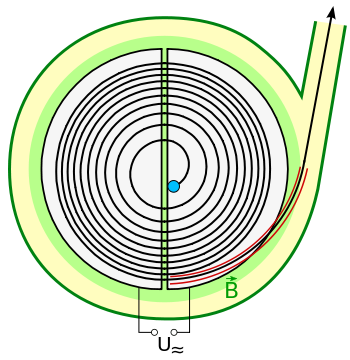
\includegraphics[width=0.35\textwidth]{Zyklotron_Prinzipskizze02.png}
%	\vspace{-13pt}
%	\caption{Prinzipskizze eines Zyklotrons}
%	\vspace{-5pt}	
%	
%\end{wrapfigure}

%\subsubsection{Anwendung}

% Some Formula:

%\begin{equation}
%	x= \frac{y \cdot 13 \pi z}
%			{\cos \alpha}
%\end{equation}

%%%%%%%%%%%%%%%%%%%%%%%
% Eigentlicher Beginn %
%%%%%%%%%%%%%%%%%%%%%%%

Eine Braun'sche Röhre wird z.B. im Bildschirm eines Oszilloskopes verwendet. Ihre Aufgabe ist es, beschleunigte Elektronen seitlich so abzulenken, dass diese auf einer bestimmten Stelle auf einem dahinter liegenden Schirm auftreffen und dort durch eine Leuchtschicht, die durch das Auftreffen von Elektronen zum Leuchten angeregt wird, sichtbar gemacht werden.

\subsection{Aufbau und Funktionsweise}

Zu Beginn müssen zunächst freie Elektronen erzeugt werden. Dies geschieht über einen Glühwendeln, ein gewickelter Draht durch den ein hoher Strom fließt. Dadurch glüht er und sondert, gemäß dem glühelektrischen Effekt\footnote{Siehe auch: \url{https://de.wikipedia.org/wiki/Edison-Richardson-Effekt}}, Elektronen ab.

Diese Elektronen werden nun mit dem elektrischen Feld einer positiv geladenen Platte beschleunigt und durch eine Loch in dieser Platte in einen oder mehrere Kondensatoren geleitet.

In diesen Kondensatoren erfolgt die eigentliche Ablenkung, gemäß der Elektronenbewegung in elektrischen Feldern (Siehe: \referenz{sec:BewegungsgesetzElektronen}). Um einen zwei-dimensionalen Schirm zu bestrahlen, müssen zwei Kondensatoren interagieren, die senkrecht zueinander stehen. Für jegliche Berechnung spart man sich dies allerdings und betrachtet nur die Ablenkung in \emph{einem} Kondensator. Siehe dazu die Abbildung \ref{fig:BraunscheRoehre} \footnote{Abbildung von \url{http://www.abi-physik.de/buch/das-elektrische-feld/braunsche-roehre/}}.

\begin{figure}[h!] 
	\centering
	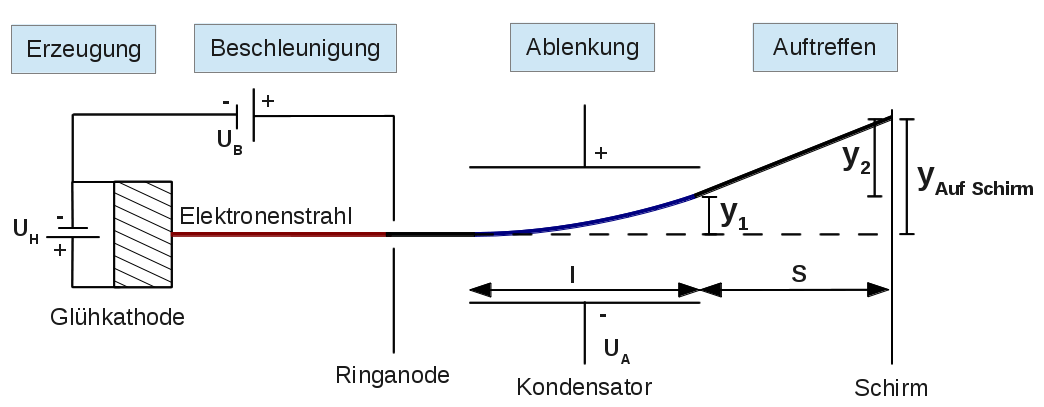
\includegraphics[width=\textwidth]{Braun}
	\caption{Schema einer Braun'schen Röhre}
	\label{fig:BraunscheRoehre}
\end{figure}

\subsection{Mathematisierung}

\subsubsection{Beschleunigungsphase}

Um auf die endgültige Geschwindigkeit der beschleunigten Elektronen in x-Richtung zu schließen, lässt sich ein Energieansatz vollziehen. Die generelle kinetische Energie $E_{kin}=\frac{1}{2}m \cdot v^2$ (wichtige Formel, die allgemein bekannt sein sollte) lässt sich der Energie des elektrischen Feldes $E_{el}=q \cdot U_B$, welches von der Platte ausgeht, gleichsetzten. Dabei ist zudem $q = q_e$ und $m = m_e$, da wir es mit Elektronen zu tun haben (Siehe \referenz{sec:Millikan} und \referenz{sec:Fadenstrahlrohr}):

\begin{align} \label{eq:BeschleunigungNachV}
\begin{split}
	E_{kin} &= E_{el} \\
	\frac{1}{2}m_e \cdot v_{x}^2 &= q_e \cdot U_B \\
	v_x &= \sqrt{\frac{2q_e \cdot U_B}{m_e}}
\end{split}
\end{align}

\begin{Aufgabe}
Oft ist die Endgeschwindigkeit gegeben und es ist nach der Spannung gefragt. Stelle die Gleichung nach der Beschleunigungsspannung $U_B$ um! Solche Umformungen sind fast das Wichtigste in der Schulphysik.
\end{Aufgabe}

\subsubsection{Ablenkungsphase}

Diese Bewegung wird wieder aufgeteilt in eine gleichförmige Bewegung in x-Richtung und eine gleichmäßig beschleunigte Bewegung in y-Richtung. Da sich dies zudem in einem Kondensator abspielt können wir exakt die Gleichung \ref{eq:y(x)imKondensator} heranziehen. Allerdings muss ,zur Abgrenzung von der Beschleunigungsspannung, zum Formelzeichen der Ablenkspannung der Index $A$ hinzugefügt werden:

\begin{align} \label{eq:y_1(x)Braun}
\begin{split}
	y_1(x) &= \frac{q_e \cdot U_A}{2d \cdot m_e} \cdot \frac{x^2}{v_{x}^2}
\end{split}
\end{align}

Jetzt kann noch die Geschwindigkeit $v_{x}$ mit der Gleichung \ref{eq:BeschleunigungNachV} ersetzt werden:

\begin{align} \label{eq:y_1(x)BraunMitV}
\begin{split}
	y_1(x) &= \frac{q_e \cdot U_A}{2d \cdot m_e} \cdot \frac{x^2 \cdot m_e}{2q_e \cdot U_B} \\
	y_1(x) &= \frac{1}{4} \cdot \frac{U_A \cdot x^2}{d \cdot U_B}
\end{split}
\end{align}


\subsubsection{Exkurs: Nach Austritt aus dem Kondensator}

Die Bewegung \emph{nach} dem homogenen elektrischen Feld bis zum Auftreffen auf dem Schirm ist die letzte Phase. Sie ist ebenfalls eine gleichförmige Bewegung, da die Elektronen in keiner Weise mehr beschleunigt werden. Allerdings besteht die Schwierigkeit hierbei, dass sie trotzdem in x- und y-Richtung unterteilt werden muss (Das Elektron wurde in Phase 2 ja schon vertikal abgelenkt). Daher muss neben der Geschwindigkeit in x-Richtung $v_x$, welche über die gesamte Bahn des Elektrons konstant ist (Siehe: \gleichungsreferenz{eq:BeschleunigungNachV}), auch die Geschwindigkeit in y-Richtung $x_{y,Austritt}$, die am Ende der Ablenkphase erreicht wird, errechnet werden. 

Die Geschwindigkeit für gleichförmig beschleunigte Bewegungen allgemein (Bewegungsgesetze!) ist die Ableitung des Wegs:

\begin{align} \label{eq:v(t)Allgemein}
\begin{split}
	v_y(t) &= a \cdot t
\end{split}
\end{align}

\noindent Auf den Kontext angewendet gilt mit $a = \frac{q_e \cdot U}{d \cdot m_e}$ (Vergleiche: Gleichung \ref{eq:y_1(x)Braun}) und $t=\frac{x}{v_x}$:

\begin{align} \label{eq:v(x)Kontext}
\begin{split}
	v_y(x) &= \frac{q_e \cdot U_A}{d \cdot m_e} \cdot \frac{x}{v_x}
\end{split}
\end{align}

\noindent Um die Geschwindigkeit in y-Richtung beim Austritt aus dem Kondensator zu berechnen, also bei dem Weg in x-Richtung, bei dem keine Beschleunigung mehr auf das Elektron wirkt, muss also die Länge des Kondensators gekannt werden und in die obige Gleichung eingesetzt werden. Sie wird hier mit $l$ abgekürzt:

\begin{align} \label{eq:v(t)Gesamt}
\begin{split}
	v_{y,Austritt} &= \frac{q_e \cdot U_A}{d \cdot m_e} \cdot \frac{l}{v_x}
\end{split}
\end{align}

\noindent Mit dieser Geschwindigkeit kann man das Bewegungsgesetz für das Elektron nach dem Austritt $y_2(x)$ aus dem Kondensator aufstellen. Dafür kommt die gleichförmige Bewegung ($y(t) = v \cdot t$) zum Einsatz:

\begin{align} \label{eq:y(t)Gesamt}
\begin{split}
	y_2(t) &= v_{y,Austritt} \cdot t \\
	y_2(t) &= (\frac{q_e \cdot U_A}{d \cdot m_e} \cdot \frac{l}{v_x}) \cdot t \\
	y_2(x) &= (\frac{q_e \cdot U_A}{d \cdot m_e} \cdot \frac{l}{v_x}) \cdot \frac{x}{v_x} \\
	y_2(x) &= \frac{q_e \cdot U_A}{d \cdot m_e} \cdot \frac{l \cdot x}{v_{x}^2}
\end{split}
\end{align}

\subsubsection{Exkurs: Gesamtgleichung}

\noindent Mit dem Abstand des Schirmes von dem Ende des Kondensators $s$ und der Beziehung für die Zeit $t=\frac{s}{v_x}$ vom Verlassen des Feldes bis zum Auftreffen auf den Schirm, kann eine Gesamtgleichung erstellt werden, die aus zwei Teilen besteht. Sie ist die Addition der Wege in y-Richtung, erstens zwischen dem Verlassen des Kondensators und dem Auftreffen auf den Schirm ($y_2(x=s)$, siehe Gleichung \ref{eq:y(t)Gesamt}) und zweitens des Weges in y-Richtung, der bereits beim Verlassen des Kondensators absolviert wurde ($y_1(x=l)$, siehe Gleichung \ref{eq:y_1(x)Braun}).

\begin{align} \label{eq:yGesamtAnsatz}
\begin{split}
	y_{Auf \ Schirm} &= y_1(x=l) + y_2(x=s) \\
	y_{Auf \ Schirm} &= \frac{q_e \cdot U_A}{2d \cdot m_e} \cdot \frac{l^2}{v_{x}^2}
				      + \frac{q_e \cdot U_A}{d \cdot m_e} \cdot \frac{l \cdot s}{v_{x}^2} \\
	y_{Auf \ Schirm} &= \frac{q_e \cdot U_A \cdot l}{d \cdot m_e \cdot v_{x}^2} \cdot (\frac{1}{2}l + s)
\end{split}
\end{align}

Als letzter Schritt wird noch für $v_{x}$ die direkte Bestimmung über die Beschleunigungsspannung $\sqrt{\frac{2 q_e \cdot U_B}{m_e}}$ aus Gleichung \ref{eq:BeschleunigungNachV} eingesetzt:

\begin{align} \label{eq:yGesamt}
\begin{split}
	y_{Auf \ Schirm} &= \frac{q_e \cdot U_A \cdot m_e}{d \cdot m_e \cdot 2 q_e \cdot U_B} \cdot (\frac{1}{2}l + s) \\
	y_{Auf \ Schirm} &= \frac{1}{2} \cdot \frac{U_A \cdot l}{d \cdot U_B} \cdot (\frac{1}{2}l + s)
\end{split}
\end{align}

\begin{Anmerkung}
Dieser Exkurs ist zwar interessant und das gekonnte Herleiten und Umstellen von Gleichungen ist in der Physik generell extrem wichtig, der Inhalt dieser Herleitung ist aber nicht klausurrelevant, dass heißt, es müssen keine Formel gelernt werden oder ähnliches. Trotzdem ist es eine anspruchsvolle und lehrreiche Aufgabe, diese Herleitung nachzuvollziehen und gegebenenfalls selbst zu vollführen.
\end{Anmerkung}






\chapter{Magnetisches Feld} \label{ch:MFeld}
\section{Beweis für die Existenz}
%%%%% Magnetisches Feld %%%%%
%% #1 Beweis für die Existenz %%


%Some sample text to be displayed above the first subsection

%\subsection{Prinzip}

%Ein Zyklotron besteht aus Zwei hohlen, halbzylindrischen und Duanden an denen eine Spannung mit unterschiedlichem Vorzeichen anliegt, und darüber bzw. darunter liegende Magneten, die ein homogenes Magnetfeld erzeugen. Zudem gibt es einen Einlass und einen Auslass für Teilchen.

%\begin{wrapfigure}{r}{0.4\textwidth} \label{Zyklo}
%
%	\vspace{-10pt}
%	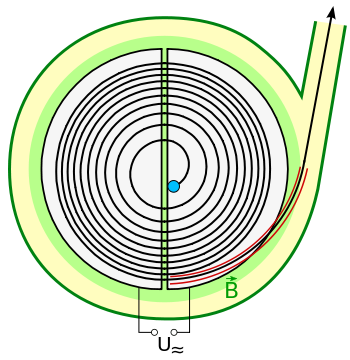
\includegraphics[width=0.35\textwidth]{Zyklotron_Prinzipskizze02.png}
%	\vspace{-13pt}
%	\caption{Prinzipskizze eines Zyklotrons}
%	\vspace{-5pt}	
%	
%\end{wrapfigure}

%\subsubsection{Anwendung}

% Some Formula:

%\begin{equation}
%	x= \frac{y \cdot 13 \pi z}
%			{\cos \alpha}
%\end{equation}

%%%%%%%%%%%%%%%%%%%%%%%
% Eigentlicher Beginn %
%%%%%%%%%%%%%%%%%%%%%%%


Man hat festgestellt, dass es noch ein weiteres Etwas mit Feldeigenschaften gibt, das Ähnlichkeiten mit dem Gravitationsfeld und dem Elektrischen Feld zeigt. Die wichtigste gemeinsame Eigenschaft ist, dass Kräfte auf bestimmte Körper ausgewirkt werden können, ohne dass es ein erkennbares Medium gibt: Der magnetische Effekt ist auch im Vakuum zu beobachten. 

Dieser Effekt kann durch eine Mehrzahl Ereignisse ausgelöst werden. (Siehe: \referenz{sec:UrsachenEigenschaften})






\section{Modellierung und Mathematisierung}
%%%%% Magnetisches Feld %%%%%
%%  %%


%Some sample text to be displayed above the first subsection

%\subsection{Prinzip}

%Ein Zyklotron besteht aus Zwei hohlen, halbzylindrischen und Duanden an denen eine Spannung mit unterschiedlichem Vorzeichen anliegt, und darüber bzw. darunter liegende Magneten, die ein homogenes Magnetfeld erzeugen. Zudem gibt es einen Einlass und einen Auslass für Teilchen.

%\begin{wrapfigure}{r}{0.4\textwidth} \label{Zyklo}
%
%	\vspace{-10pt}
%	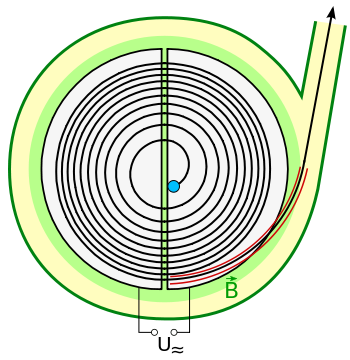
\includegraphics[width=0.35\textwidth]{Zyklotron_Prinzipskizze02.png}
%	\vspace{-13pt}
%	\caption{Prinzipskizze eines Zyklotrons}
%	\vspace{-5pt}	
%	
%\end{wrapfigure}

%\subsubsection{Anwendung}

% Some Formula:

%\begin{equation}
%	x= \frac{y \cdot 13 \pi z}
%			{\cos \alpha}
%\end{equation}

%%%%%%%%%%%%%%%%%%%%%%%
% Eigentlicher Beginn %
%%%%%%%%%%%%%%%%%%%%%%%


\subsection{Feldlinien}

Wie schon beim elektrischen Feld wird hier ein Feldlinienmodell genutzt um Eigenschaften wie Ausrichtung (Polung) oder Stärke darzustellen. 

Magnetische Felder haben 2 Pole, die nicht negativ oder positiv, wie beim elektrischen Feld, sondern Nord- und Südpol genannt werden. Ungleichnamige Pole ziehen sich an, gleichnamige stoßen sich ab. Im Feldlinienmodell zeigen die Pfeile immer zum Südpol.

Charakteristische Bilder von Feldlinien sowie Erklärungen zu diesen finden sich in \referenz{sec:feldlinienbilder}.


\subsection{Magnetische Flussdichte}

Auch beim magnetischen Feld gibt die Dichte der Feldlinien eine Größe für die Stärke des Feldes an. Diese Größe heißt aber nicht Feldstärke sondern \glqq magnetische Flussdichte \grqq{} (Formelzeichen $B$, Einheit \glqq Telsa\grqq : $T=\frac{kg}{As^2}=\frac{Vs}{m^2}$) (die magnetische Feldstärke gibt es auch, bezeichnet aber etwas anderes!). Diese ist also äquivalent zur Feldstärke des elektrischen Feldes und ordnet über die Lorentzkraft (Siehe: \referenz{sec:lorenzkraft}) jedem bewegten, geladenen Teilchen eine Kraft zu (Siehe \referenz{subsec:BLorentzDefinition}).


\subsection{Homogenes Feld} \label{subsec:MFeldHomogen}

Ein homogenes Magnetfeld hat die Eigenschaft, dass die Flussdichte in jedem Punkt gleich ist, was Berechnungen erheblich einfacher macht (Vergleiche: \referenz{subsec:EFeldHomogen}). Homogene Felder treten zum Beispiel im Inneren von Spulen oder zwischen den Schenkeln eines Hufeisenmagneten auf. Mehr dazu in \referenz{sec:feldlinienbilder}.



















\section{Ursachen und Eigenschaften eines Magnetfeldes} \label{sec:UrsachenEigenschaften}
\subsection{Ferromagnetisches Metall}

Ein magnetisches Feld wird im klassischsten Sinne ausgelöst, wenn ein ferromagnetisches Metall \glqq magnetisiert\grqq{} wird, was heißt, dass sich sogenannte Elementarmagnete ausrichten.\footnote{Siehe: \url{https://de.wikipedia.org/wiki/Elementarmagnet}}


\subsection{Elektromagnet}

Jegliche Leiter, auch nicht-ferromagnetischer Natur, lösen ein magnetisches Feld aus, wenn Strom durch sie fließt.

Wenn Strom (also Elektronen, die kleinste Einheit der negativen Ladung) durch einen Leiter fließt, ergibt sich ein magnetisches Feld, dessen Ausrichtung gemäß verschiedener Handregeln erfolgt. Siehe dazu \referenz{subsec:Faustregel}.


\subsection{Erdmagnetfeld}

Auch von der Erde geht ein magnetisches Feld aus, welches z.B. für Kompanten genutzt wird.



\section{Feldlinienbilder} \label{sec:feldlinienbilder}
\subsection{Faustregel}	\label{subsec:Faustregel}

Als Eselsbrücke zur Bestimmung der Richtung der Feldlinien um den stromdurchflossenen Leiter kann die \glqq Faustregel\grqq{} herangezogen werden. Diese besagt, dass bei der physikalischen Stromrichtung (auch Elektronenflussrichtung genannt) die Feldlinien in Richtung der Fingerspitzen der linken Hand verlaufen, wenn nur der Daumen von der Faust abgespreizt wird und die Flussrichtung angibt.

Für die technische Stromrichtung gilt dieselbe Regel, bloß, dass mit der rechten Faust verfahren wird.

\begin{leftbar}
	Wichtig! Die physikalische Stromrichtung geht von der Bewegung der Elektronen, also der negativen Ladung aus. Diese fließen vom Minuspol zum Pluspol. Die technische Stromrichtung dagegen geht davon aus, dass die positiven Ladungen sich vom Pluspol zum Minuspol bewegen. Durch die Verwendung gespiegelter Handregeln (die jeweils andere Hand wird genommen) bleiben die Effekte jedoch dieselben. 
	
	Allgemein wird in der Physik die physikalische Stromrichtung und damit die \emph{linken} Handregeln bevorzugt, da es auch wirklich die Elektronen sind, die sich in einem Leiter bewegen.
\end{leftbar}

\subsection{Dauermagneten}  	\label{subsec:DauermagnetFeld}

\hfill

\begin{figure}[ht!]
	\centering
	\begin{minipage}[b]{0.4\linewidth}
    	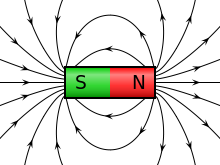
\includegraphics[width=\textwidth]{Stabmagnet}
		\caption{Das Magnetfeld um einen Stabmagnet.}
	\end{minipage}
	\quad
	\begin{minipage}[b]{0.4\linewidth}
    	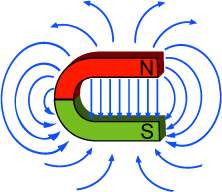
\includegraphics[width=0.6\textwidth]{Hufeisen}
		\caption{Das Magnetfeld an einem Hufeinenmagnet. Interessant ist der homogene Bereich zwischen den Schenkeln.}
	\end{minipage}
\end{figure}


\subsection{Gerader Leiter} 
\footnote{\url{https://lp.uni-goettingen.de/get/text/3791}} 
\footnote{„Gerader leiter“ von Talos aus der deutschsprachigen Wikipedia. Lizenziert unter CC BY-SA 3.0 über Wikimedia Commons - \url{https://commons.wikimedia.org/wiki/File:Gerader_leiter.svg}} 
\footnote{„Stromschleife“ von 30px MovGP0 - selbst erstellt mit Inkscape. Lizenziert unter CC BY-SA 2.0 de über Wikimedia Commons - \url{https://commons.wikimedia.org/wiki/File:Stromschleife.svg}} 
\label{subsec:GeraderLeiterFeld}

\hfill

\begin{figure}[ht!]
	\centering
	\begin{minipage}[b]{0.4\linewidth}
   	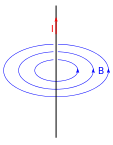
\includegraphics[width=\textwidth]{GeraderLeiter}
		\caption{Das Magnetfeld um einen geraden Leitern. $I$ zeigt die \emph{technische} Stromrichtung an.}
	\end{minipage}
	\quad
	\begin{minipage}[b]{0.4\linewidth}
    	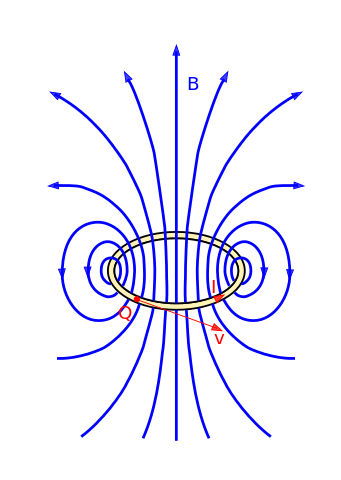
\includegraphics[width=\textwidth]{Stromschleife}
	\caption{Das Magnetfeld um eine Leiterschleife (Spule mit nur einer Windung). Man nehme Notiz von der Art, wie sich die einzelnen Feldlinien um den Leiter herum in der Mitte zu einem Bündel Feldlinien akkumulieren. $I$ zeigt die \emph{technische} Stromrichtung an.}
	\end{minipage}
\end{figure}

\newpage

\subsection{Spule} \label{subsec:MFeldSpule}
\footnote{„VFPt cylindrical coil real“ von Geek3 - Eigenes WerkThis plot was created with VectorFieldPlot. Lizenziert unter CC BY-SA 3.0 über Wikimedia Commons - \url{https://commons.wikimedia.org/wiki/File:VFPt_cylindrical_coil_real.svg}}
\label{subsec:Spule}

\hfill

\begin{figure}[ht!]
	\centering
   	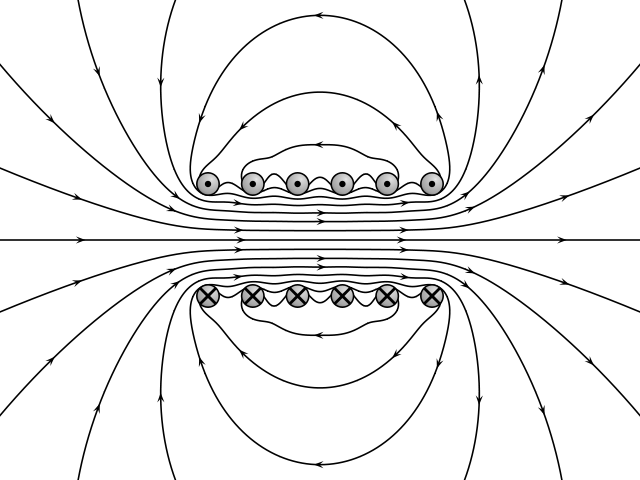
\includegraphics[width=0.8\textwidth]{Spule}
		\caption{Das Magnetfeld im Inneren einer Spule. Im Querschnitt zeigt $\otimes$ den technischen Stromfluss in die Blattebene an. Vergleichbar mit der Leiterschleife, aber mit deutlich homogenerem Fluss im Inneren.}
\end{figure}





\section{Lorentzkraft} \label{sec:lorentzkraft}
%%%%% Magnetisches Feld %%%%%
%%  %%


%Some sample text to be displayed above the first subsection

%\subsection{Prinzip}

%Ein Zyklotron besteht aus Zwei hohlen, halbzylindrischen und Duanden an denen eine Spannung mit unterschiedlichem Vorzeichen anliegt, und darüber bzw. darunter liegende Magneten, die ein homogenes Magnetfeld erzeugen. Zudem gibt es einen Einlass und einen Auslass für Teilchen.

%\begin{wrapfigure}{r}{0.4\textwidth} \label{Zyklo}
%
%	\vspace{-10pt}
%	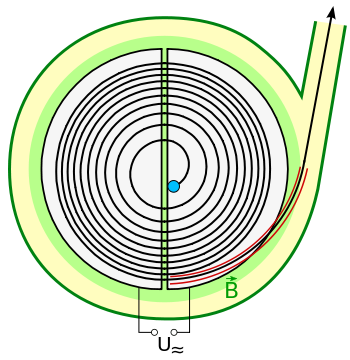
\includegraphics[width=0.35\textwidth]{Zyklotron_Prinzipskizze02.png}
%	\vspace{-13pt}
%	\caption{Prinzipskizze eines Zyklotrons}
%	\vspace{-5pt}	
%	
%\end{wrapfigure}

%\subsubsection{Anwendung}

% Some Formula:

%\begin{equation}
%	x= \frac{y \cdot 13 \pi z}
%			{\cos \alpha}
%\end{equation}

%%%%%%%%%%%%%%%%%%%%%%%
% Eigentlicher Beginn %
%%%%%%%%%%%%%%%%%%%%%%%

\subsection{Geladenes Teilchen}

Die Lorentzkraft wirkt auf jedes geladene, in einem Magnetfeld bewegte Teilchen, wenn sich dieses Teilchen nicht parallel zu den Feldlinien bewegt. Die Lorentzkraft ist abhängig von der Flussdichte des Magnetfeldes, der Ladung und Geschwindigkeit des Teilchens und von dem Winkel zu den Feldlinien. Im Folgenden werden jedoch nur noch Fälle betrachtet, bei denen sich Teilchen senkrecht zu den Feldlinien bewegen, was Berechnungen vereinfacht.


\subsection{Stromdurchflossener Leiter}

Durch einen stromdurchflossenen Leiter fließen Elektronen vom Minuspol zum Pluspol. Da Elektronen negativ geladene Teilchen sind, wirkt auch in diesem Fall die Lorentzkraft auf den Leiter, wenn sich der Leiter in einem magnetischen Feld befindet.

\subsection{Handregeln}

\begin{figure}[h!]
	\centering
	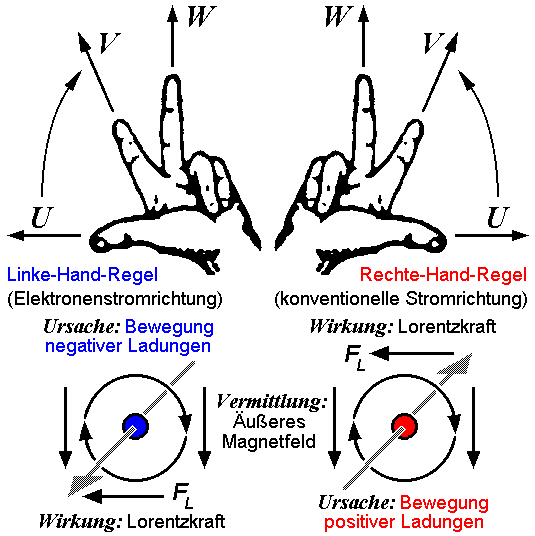
\includegraphics[width=0.65\textwidth]{Handregeln}
	\caption{Die beiden Handregeln für negative und die positive Teilchen. Die Linke gilt zudem für die physikalische und die Rechte für die Technische Stromrichtung. U: Ursache, V: Vermittlung, W: Wirkung}
	\label{fig:Handregeln}
\end{figure}

Bei der Richtung der Lorentzkraft auf ein negativ geladenes Teilchen, das sich senkrecht zu den Feldlinien eines magnetischen Feldes bewegt, gilt die linke Handregel. Bei dieser werden Daumen, Zeige- und Mittelfinger der linken Hand abgespreizt, sodass sie der Zeichnung \ref{fig:Handregeln}\footnote{„UVWREGEL new“ von UVWREGEL.png: Qniemiec 19:15, 14. Jan. 2011 (CET).Original uploader was Qniemiec at de.wikipediaderivative work: Qniemiec (talk) - UVWREGEL.png. Lizenziert unter CC BY-SA 3.0 über Wikimedia Commons - \url{https://commons.wikimedia.org/wiki/File:UVWREGEL_new.png}} entsprechen. Dann bezeichnet der Daumen die Richtung des Teilchens, der Zeigefinger folgt der Richtung des Magnetfeldes und der Mittelfinder zeigt schlussendlich die Richtung der Lorentzkraft an. Für die Kraft auf einen Leiter, der senkrecht in einem Magnetfeld steht, gilt dieselbe Regel wobei der Daumen die physikalische Stromrichtung anzeigt.

Für ein positives Teilchen oder die technische Stromrichtung in einem Leiter kommt die rechte Hand zum Einsatz; die Regel für die Bezeichnung der Finger bleibt gleich.


\subsection{Gleichung} \label{subsec:BLorentzDefinition}

Der Betrag der Lorentzkraft lässt sich wie folgt berechnen:

\begin{align} \label{eq:Lorentzkraft}
\begin{split}
	F_{Lr} = q \cdot B \cdot v
\end{split}
\end{align}

\begin{NiceToKnow}
	Es wird zwar im Unterricht nicht, behandelt, ist aber eventuell ein Fall für eine Transferaufgabe im Abitur: Die Lorenzkraft auf ein geladenes Teilchen, welches sich nicht senkrecht zu den Feldlinien bewegt, ist abhängig vom Sinus aus dem Winkel zwischen der Bewegungsrichtung und der Feldlinien, also der Magnetfeldrichtung:

	\begin{equation}
		F_{Lr} = q \cdot B \cdot v \cdot \sin{(\angle{\vec{v}, \vec{B}})}
	\end{equation}

	\noindent Mit dem Kreuzprodukt geschrieben:

	\begin{equation}
		F_{Lr} = q \cdot (\vec{B} \times \vec{v})
	\end{equation}
\end{NiceToKnow}

\noindent Interessant ist, dass die Lorentzkraft nicht nur von der Ladung, sondern auch von der Geschwindigkeit des Teilchens abhängig ist. Dies macht man sich z.B. im Massenspektrometer (Siehe: \referenz{sec:Massenspektrometer}) oder im Wien'schen Filter (Siehe: \referenz{sec:Wien}) zu Nutze.

Aus der Lorentzkraft lässt sich auch die Flussdichte $B$ definieren: Die Flussdichte ordnet jedem bewegten, geladenen Körper eine Kraft (die Lorentzkraft) zu:

\begin{align} \label{eq:Flussdichte}
\begin{split}
	\vec{B} = \frac{\vec{F}_{Lr}}{q \cdot \vec{v}}
\end{split}
\end{align}

\noindent Daraus folgt auch die Einheit Tesla der Flussdichte:

\begin{align} \label{eq:Flussdichte}
\begin{split}
	T &= N \cdot \frac{1}{C \cdot \frac{m}{s}} \\
	T &= \frac{kg \cdot m}{s^2} \cdot \frac{s}{As \cdot m} \\
	T &= \frac{kg}{As^2}	
\end{split}
\end{align}







\section[Fadenstrahlrohr]{Spezifische Ladung und Elektronenmasse per Fadenstrahlrohr} \label{sec:Fadenstrahlrohr}
Das Fadenstrahlrohr illustriert die Lorentzkraft und diente zur Bestimmung der spezifischen Elektronenladung ($\frac{q_e}{m_e}$). Zusammen mit den Ergebnissen des Millikanversuchs (siehe: \referenz{sec:Millikan}) kann sogar die Masse eines Elektrons bestimmt werden.

\subsection{Aufbau}

\begin{figure}[h!]
	\centering
	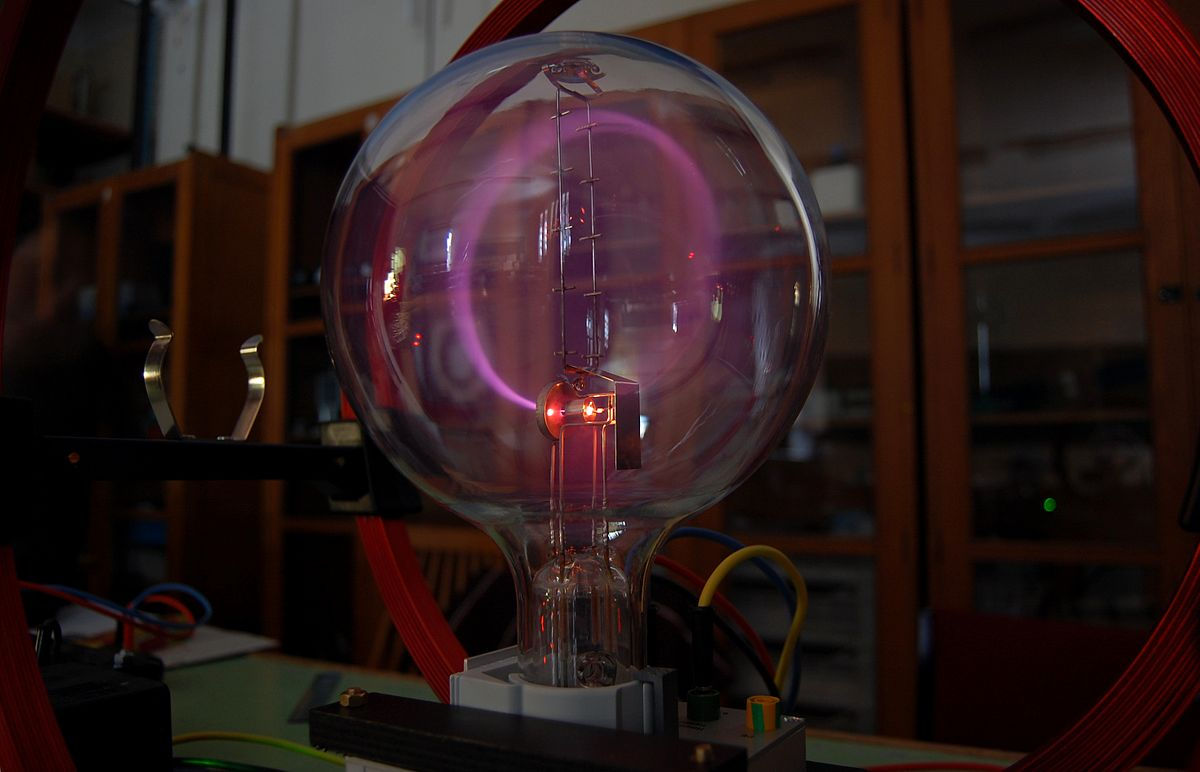
\includegraphics[width=0.7\textwidth]{Fadenstrahlrohr}
	\caption{Ein Fadenstrahlrohr: Das leuchtende Gas zeight die Elektronenbahn an.}
	\label{fig:Fadenstrahlrohr}
\end{figure}

Ein Fadenstrahlrohr besteht aus einem Glaskolben in dem sich ein Gas befindet, welches beim Kontakt mit Elektronen zum Leuchten angeregt wird. Siehe Abbildung \ref{fig:Fadenstrahlrohr}\endnote{„Cyclotron motion wider view“ von Marcin Białek - Eigenes Werk. Lizenziert unter GFDL über Wikimedia Commons - \url{https://commons.wikimedia.org/wiki/File:Cyclotron\_motion\_wider\_view.jpg}}

Im Inneren befindet sich eine Elektronenkanone, die beschleunigte Elektronen absondert (Siehe: \referenz{sec:BraunscheRoehre}). Durch ein \emph{Helmholzspulenpaar} (2 kurze Spulen mit großem Radius) die parallel zur Richtung der beschleunigten Elektronen stehen, wird ein homogenes Magnetfeld erreicht, welches senkrecht auf der Elektronenrichtung steht.

\subsection{Beobachtung}

Die Elektronen beschreiben eine Kreisbahn, was am leuchtenden Gas zu sehen ist. Damit ist die Existenz einer Kraft auf bewegte, geladene Teilchen im Magnetfeld illustriert.

\subsection{Mathematisierung}

Wenn die Geschwindigkeit der Elektronen bekannt, bzw. errechnet wurde, kann über den Radius, welcher auch gemessen werden kann, die spezifische Elektronenladung bestimmt werden. Der Ansatz ist das Gleichsetzten der allgemeinen Zentripetalkraft $F_{Zp} = m \cdot \frac{v^2}{r}$, also die Kraft, die aufgewendet werden muss, um ein Elektron auf der Bahn zu halten, mit der Lorentzkraft  $F_{Lr} = q \cdot B \cdot v$, welche ja genau diese Bahn bewirkt:

\begin{align}
\begin{split}
	F_{Zp} &= F_{Lr} \\
	m_e \cdot \frac{v^2}{r} &= q_e \cdot B \cdot v \\
	\frac{q_e}{m_e} &=\frac{v}{B \cdot r}
\end{split}
\end{align}

\noindent Da es 2 Variablen in der Gleichung gibt ($m_e$ und $q_e$), kann man mit diesem Versuch nur auf das \emph{Verhältnis} der Ladung und Masse schließen, die \glqq spezifische Elektronenmasse\grqq .

Über den Millikanversuch (siehe: \referenz{sec:Millikan}) konnte jedoch die Elektronenladung $q_e$ direkt bestimmt werden, sodass durch den Versuch mit dem Fadenstrahlrohr die Masse bestimmt werden konnte:

\begin{align}
\begin{split}
	\frac{q_e}{m_e} &=\frac{v}{B \cdot r} \\
	m_e &=\frac{q_e \cdot B \cdot r}{v}
\end{split}
\end{align}







\section{Wien'scher Geschwindigkeitsfilter} \label{sec:Wien}
Der Wien'sche Geschwindigkeitsfilter ist eine Möglichkeit, einen Elektronenstrahl nach seiner Geschwindigkeit zu filtern, das heißt, nur Elektronen mit einer gewissen Geschwindigkeit passieren zu lassen.

\subsection{Aufbau}


Grundbaustein bildet eine Ablenkeinheit mit einem Kondensator, wie sie in der Braun'schen Röhre (Siehe: \referenz{sec:BraunscheRoehre}) verwendet wird. Allerdings wird nun ein homogenes Magnetfeld so über den Kondensator gelegt, dass die Feldlinien dieses Feldes senkrecht auf der Elektronenrichtung \emph{und} den Feldlinien des elektrischen Feldes stehen.

Abbildung \ref{fig:Wien}\endnote{„Wienscher Geschwindigkeitsfilter“ von Till Blaha - Eigenes Werk. Lizenziert unter Gemeinfrei} zeigt den schematischen Aufbau und die grobe Funktionsweise für einen Versuch mit Elektronen.

\begin{figure}[h!]
	\centering
	\vspace*{-10pt}
	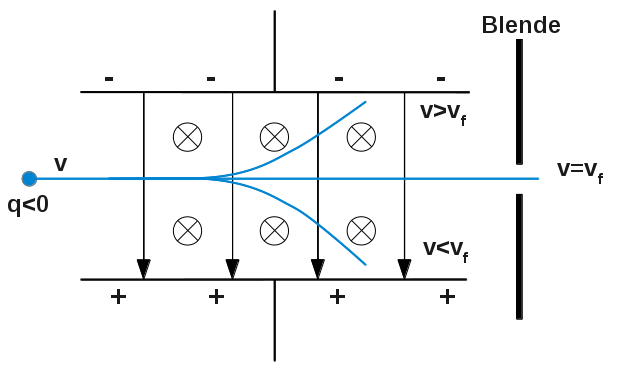
\includegraphics[width=0.8\textwidth]{WienscherFilter}
	\caption{Der Geschwindigkeitsfilter nach Wien. Die Pfeile charakterisieren die Richtung des elektrischen Feldes, die Kreuze zeigen an, dass die Richtung des Magnetfeldes in die Blattebene verläuft.}
	\label{fig:Wien}
\end{figure}

\begin{Anmerkung}
	Die magnetischen Feldlinien sind nicht direkt zeichenbar, da sie \glqq in die Papierebene\grqq{} gehen. Es wird $\odot$ verwendet, um Anzuzeigen, dass der Pfeil aus der Ebene hinaus verläuft und $\otimes$ um Anzuzeigen, dass der Pfeil in die Ebene hinein verläuft.
	
	Eselsbrücke: Wenn man mit einem Bogen einen Pfeil verschießt, sie man das Kreuz der Federn; im letzten Moment, bevor man von einem getroffen wird, sieht man den Punkt der Pfeilspitze.
\end{Anmerkung}



\subsection{Funktionsweise}

Das Magnetfeld und der Kondensator werden so gepolt, dass die, gemäß linker Handregel resultierende, Lorentzkraft $F_{Lr}$ der Coulombkraft $F_{el}$ entgegenwirkt. Da die Lorentzkraft abhängig von der Geschwindigkeit des Elektrons ist und die elektrische Kraft nicht, gibt es eine Geschwindigkeit $v_f$, bei der sich die beiden Kräfte die Waage halten. Dies ist die Geschwindigkeit, die vom Filter durchgelassen wird:

\begin{align}
\begin{split}
	F_{Lr} &= F_{el} \\
	q_e \cdot B \cdot v_f &= q_e \cdot E \\
	v_f &= \frac{E}{B}
\end{split}
\end{align}

\noindent \emph{Man nehme Notiz von dieser simplen und unglaublich schönen Beziehung!}

Eine Einheitenrechnung folgt und zeigt, dass die Einheiten aufgehen:

\begin{align}
\begin{split}
	v_f &= \frac{E}{B} \\
	\frac{m}{s} &= \frac{N}{C} \cdot \frac{1}{T} \\
	\frac{m}{s} &= \frac{kg \cdot m}{s^2 \cdot As} \cdot \frac{As^2}{kg} \\
	\frac{m}{s} &= \frac{m}{s}
\end{split}
\end{align}


\section{Massenspektrometer} \label{sec:Massenspektrometer}
%%%%% Magnetisches Feld %%%%%
%% Massenspektrometer %%


%Some sample text to be displayed above the first subsection

%\subsection{Prinzip}

%Ein Zyklotron besteht aus Zwei hohlen, halbzylindrischen und Duanden an denen eine Spannung mit unterschiedlichem Vorzeichen anliegt, und darüber bzw. darunter liegende Magneten, die ein homogenes Magnetfeld erzeugen. Zudem gibt es einen Einlass und einen Auslass für Teilchen.

%\begin{wrapfigure}{r}{0.4\textwidth} \label{Zyklo}
%
%	\vspace{-10pt}
%	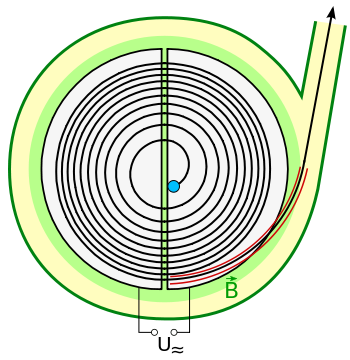
\includegraphics[width=0.35\textwidth]{Zyklotron_Prinzipskizze02.png}
%	\vspace{-13pt}
%	\caption{Prinzipskizze eines Zyklotrons}
%	\vspace{-5pt}	
%	
%\end{wrapfigure}

%\subsubsection{Anwendung}

% Some Formula:

%\begin{equation}
%	x= \frac{y \cdot 13 \pi z}
%			{\cos \alpha}
%\end{equation}

%%%%%%%%%%%%%%%%%%%%%%%
% Eigentlicher Beginn %
%%%%%%%%%%%%%%%%%%%%%%%

Das Massenspektrometer macht man sich zur Identifikation von chemischen Elementen und deren Isotopen die unterschiedlichen Atommassen zu Nutze. Die ersten funktionstüchtigen Massenspektrometer gibt es seit dem frühen 20. Jahrhundert.

\subsection{Aufbau}

In der Ionenquelle werden Atome aus der Probe gelöst und ionisiert. Das heißt, sie sind nun im gasförmigen Zustand und zudem positiv geladen.

Nach einer Beschleunigungseinheit und einem Wien'schen Filter werden sie in ein homogenes Magnetfeld geleitet in welchem sie dann, gemäß der Lorentzkraft auf eine Kreisbahn gezwungen werden. 

Da man absolute Gewissheit über Ladung, Geschwindigkeit hat und auch die Flussdichte des Magnetfeldes kennt, ist die einzige Variable, die den Auftreffpunkt auf der Indikatorplatte bestimmt, die Masse des Atoms. Wie beim Fadenstrahlrohr (Siehe \referenz{sec:Fadenstrahlrohr}) wird der Ansatz $F_{Zp} = F_{Lr}$ vollzogen:

\begin{align}
\begin{split}
	F_{Zp} 				  &= F_{Lr} \\
	m \cdot \frac{v^2}{r} &= q \cdot B \cdot v \\
	m 					  &= \frac{q \cdot B \cdot r}{v}
\end{split}
\end{align}












\section{Zyklotron}
%%%%% Magnetisches Feld %%%%%
%%  %%


%Some sample text to be displayed above the first subsection

%\subsection{Prinzip}

%Ein Zyklotron besteht aus Zwei hohlen, halbzylindrischen und Duanden an denen eine Spannung mit unterschiedlichem Vorzeichen anliegt, und darüber bzw. darunter liegende Magneten, die ein homogenes Magnetfeld erzeugen. Zudem gibt es einen Einlass und einen Auslass für Teilchen.

%\begin{wrapfigure}{r}{0.4\textwidth} \label{Zyklo}
%
%	\vspace{-10pt}
%	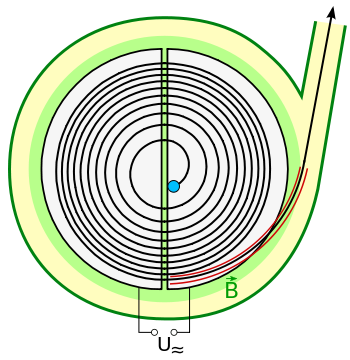
\includegraphics[width=0.35\textwidth]{Zyklotron_Prinzipskizze02.png}
%	\vspace{-13pt}
%	\caption{Prinzipskizze eines Zyklotrons}
%	\vspace{-5pt}	
%	
%\end{wrapfigure}

%\subsubsection{Anwendung}

% Some Formula:

%\begin{equation}
%	x= \frac{y \cdot 13 \pi z}
%			{\cos \alpha}
%\end{equation}

%%%%%%%%%%%%%%%%%%%%%%%
% Eigentlicher Beginn %
%%%%%%%%%%%%%%%%%%%%%%%

\subsection{Prinzip} 

Ein Zyklotron besteht aus 2 hohlen, halbzylindrischen Duanden, an denen eine Spannung mit unterschiedlichem Vorzeichen anliegt. Zwischen den Duanden befindet sich ein kleiner Zwischenraum, in welchem dann ein homogenes elektrisches Feld entsteht, dessen Feldlinien von der einen zur anderen Duande verlaufen (Siehe \referenz{subsec:EFeldHomogen}). Aus 2 darüber bzw. darunter liegenden Magneten ergibt sich ein homogenes Magnetfeld (Siehe \referenz{subsec:MFeldHomogen}).

Darüber hinaus gibt es einen Einlass und einen Auslass für Teilchen.\footnote{„Zyklotron Prinzipskizze02“ von KlausFoehl - Eigenes Werk. Lizenziert unter Gemeinfrei über Wikimedia Commons - \url{https://commons.wikimedia.org/wiki/File:Zyklotron_Prinzipskizze02.svg}}


\begin{wrapfigure}{o}{0.4\textwidth} \label{Zyklo}

	\vspace{-10pt}
	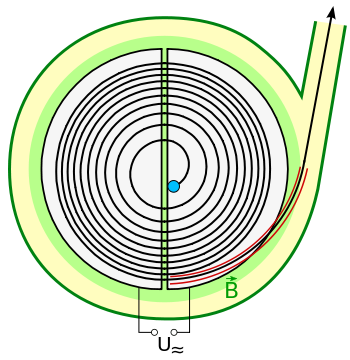
\includegraphics[width=0.35\textwidth]{Zyklotron_Prinzipskizze02.png}
	\vspace{-13pt}
	\caption{Prinzipskizze eines Zyklotrons}
	\vspace{-5pt}	
	
\end{wrapfigure}

Die Teilchenquelle im Inneren des Zyklotrons setzt Elektronen oder Protonen frei, welche durch den Einlass in das elektrische Feld zwischen den Duanden eintreten und durch dieses Feld zu einer der Beiden hin beschleunigt werden. Diese Teilchen werden gleichzeitig durch das Magnetfeld, über die Lorentzkraft, auf eine Kreisbahn gezwungen (Siehe \referenz{sec:lorentzkraft}), sodass sie im hohlen Duanden eine 180\degree{} Kurve beschreiben. Sobald wieder der Spalt zwischen den Duanden erreicht ist, wird die Spannung umgepolt, sodass die Teilchen nun zum anderen Duanden hingezogen werden. Diese Umpolungsfrequenz bleibt über den ganzen Versuch konstant.

In dem Spalt werden die Teilchen abermals und abermals beschleunigt bis der Radius so groß ist, dass die Teilchen aus dem Zyklotron austreten.


\subsection{Gesetze}

Für die Beschleunigung für \emph{Elektronen} gelten folgende Gesetzmäßigkeiten.

\subsubsection{Radius}

Aus der Gleichsetzung der Zentrifugalkraft und der Lorentzkraft ergibt sich: 

\begin{align}
\begin{split}
	F_{Zf} &= F_{Lr} \\
	\frac{m \cdot v^2}{r} &= q_e \cdot v \cdot B
\end{split}
\end{align}

\noindent Daher gilt für den Radius:

\begin{align} \label{eq:ZyklotronRadius}
\begin{split}
	r = \frac{m_e \cdot v}{B \cdot q_e}
\end{split}
\end{align}


\subsubsection{Frequenz}

Aus den Betrachtungen der Umlaufzeit $T = \frac{s_{Umlauf}}{v} = \frac{2 \pi r}{v}$ und des Radius (Siehe Gleichung \ref{eq:ZyklotronRadius}) ergibt sich für die Frequenz der Umpolung mit $f=\frac{1}{T}$: \\

\begin{align}
\begin{split}
	f &= \frac{1}{T} \\
	f &= \frac{v}{2 \pi r} \\
	f &= \frac{v \cdot q_e \cdot B}{2 \pi \cdot m_e \cdot v} \\
	f &= \frac{q_e \cdot B}{2 \pi \cdot m_e}
\end{split}
\end{align}

\noindent Damit ist gezeigt, dass die Frequenz nicht abhängig von der Geschwindigkeit der Teilchen ist und auch sonst nur von konstanten Größen abhängig ist. Daher ist die Frequenz über den gesamten Versuch konstant.






\chapter{Induktion} \label{ch:Induktion}
\section{Grundprinzip}

Induktion bezeichnet die Entstehung eines elektrischen Feldes, bzw. einer Spannung, durch die Änderung eines Magnetfeldes. Das heißt, wenn sich die Flussdichte eines Magnetfeldes ändert, ist in einem elektrischen Leiter, der sich in diesem Feld befindet, eine Spannung messbar. Obwohl die Induktivität einer Spule deutlich höher ist, wird eine Spannung auch in einem beliebigem Leiter induziert.


\section{Induktionsgesetz}

Für die Induktionsspannung gilt in Spulen:

\begin{equation} \label{eq:InduGe}
	U_{ind} = -N \frac{d\phi}{dt}
\end{equation}

\noindent Wobei: $\phi = B \cdot A$ (sprich: \glqq klein Phi\grqq).

Für die Induktionsspannung gilt für bewegte Leiter mit $\vec{v} \perp \vec{B}$:

\begin{equation}
	U_{ind} = -B \cdot l \cdot v
\end{equation}


\section{Verlauf der Induktionsspannung}

Sollte sich bei einem Experiment ein Permanentmagnet durch eine Spule bewegen, die länger ist als er selbst, steigt die Induktionsspannung beim Eintritt schnell an. Sobald sich mehr als die Hälfte der Fläche des Magneten in der Spule befindet, nimmt die Spannung ab und solange er vollständig in der Spule ist beträgt die Spannung $0V$, da sich das Magnetfeld in der Spule nun nicht mehr ändert. Beim Austreten nimmt die Spannung wieder zu, diesmal jedoch in der entgegengesetzten Richtung, die Änderung des Magnetfeldes $\Delta B$ nun negativ ist.


\section{Lenz'sche Regel}

Die Lenz'sche Regel besagt, dass eine Spannung immer dem Magnetfeld entgegengesetzt induziert wird. Daher stammen auch die Negationen in den Induktionsgesetzen.

Da eine Spule in einem geschlossenen Stromkreis, in der eine Spannung induziert wurde, ein Strom fließt, der selbst ein Magnetfeld erzeugt, muss dieses Magnetfeld, gemäß der Energieerhaltung dem induzierenden Magnetfeld entgegengesetzt sein. Beispielsweise würde sonst ein Magnet, der sich durch eine Spule bewegt, durch das Magnetfeld der Spule, das er selbst induzierte, noch immer weiter beschleunigt werden; ein unmögliches perpetuum Mobile. \label{sec:Lenz}


\section[Lange Spulen]{Magnetischer Fluss in Langen Spulen}

\subsection{Definition}

Lange Spulen sind gerade und deren Länge ist größer als deren Durchmesser. Damit ist im Inneren ein homogenes Magnetfeld zu beobachten, siehe \referenz{sec:feldlinienbilder}.


\subsection{Gesetze}

Die magnetische Flussdichte im Inneren einer stromdurchflossenen Spule in definiert als:

\begin{equation} \label{eq:MaFluss}
	B = 	\mu_0 \mu_r \cdot N \cdot \frac{I}{l}
\end{equation}

\noindent Hierbei ist $\mu_0$ die magnetische Permeabilitätskonstante und $mu_r$ die relative Permeabilitätszahl, welche für Luft und Vakuum $\approx 1$ ist. 

\begin{NiceToKnow}
Mit speziellen Legierungen können relative Permeabilitäten von über $9 \cdot 10^5$ erreicht werden, was die Flussdichte um den selben Faktor erhöhen würde.
\end{NiceToKnow}


\section{Induktivität}

Die Induktivität beschreibt die Größe des Vermögens von elektrischen Leitern, insbesondere Spulen, zu Induzieren.

\subsection{Definition und Gesetz}

Für Spulen gilt:

\begin{equation} \label{eq:Invitat}
	L = \mu_0 \mu_r \frac{N^2 \cdot A}{l}
\end{equation}

Wobei $\mu_r$ (sprich \glqq klein Mü\grqq ) die relative Permeabilität des Spulenkerns ist; bei Luft bzw. Vakuum gilt $ \mu_r \approx 1$. 


\subsection{Induktionsgesetz mit der Induktivität}

Nach Einsetzen und Kürzen von der magnetischen Flussdichte (siehe Gleichung \ref{eq:MaFluss} auf Seite \pageref{eq:MaFluss}) in die Formel für Induktion (siehe Gleichung \ref{eq:InduGe} auf Seite \pageref{eq:InduGe}) ergibt sich:

\begin{equation}
	U_{ind} = - \mu_0 \mu_r \cdot \frac{N^2}{l}
				\cdot A \cdot \frac{dI}{dt}
\end{equation}

Auffallend ist, dass der Teil $\mu_0 \mu_r \cdot \frac{N^2}{l} \cdot A$ die eben benannte Induktivität ist (siehe Gleichung \ref{eq:Invitat}). Daher kann die Induktionsspannung auch wie folgt berechnet werden:

\begin{equation}
	U_{ind} = - L \cdot \frac{dI}{dt}
\end{equation}


\section{Selbstinduktion}	\label{sec:Selbstinduktion}

\subsection{Grundprinzip}

Wenn Elektronen durch einen Leiter fließen, erzeugen sie einen Strom, der in einer Spule ein Magnetfeld aufbaut (Siehe \referenz{subsec:MFeldSpule}). Beim Aufbau dieses Magnetfeldes ändert sich dieses, logischerweise. Diese Änderung erzeugt allerdings in der selben Spule auch wieder eine Induktion, die sogenannte Selbstinduktion, deren Strom gemäß der Lenz'schen Regel (Siehe \referenz{sec:Lenz}) entgegengesetzt der eigentlichen Stromrichtung gerichtet ist.

Dies führt dazu, dass der Stromfluss "gebremst" wird.

\subsection{Verhalten beim Unterbrechen eines Stromkreises}

Wenn in einem Stromkreis eine Spule mit Strom durchflossen wurde und sich in ihr das Magnetfeld vollständig aufgebaut hat, wird bei einer abrupten Unterbrechung des Stromkreises das Magnetfeld zusammenbrechen und aufgrund dieser starken Änderung ($\Delta t$ ist sehr klein) eine hohe, entgegengesetzt gepolte Spannung induziert.

\begin{figure}
	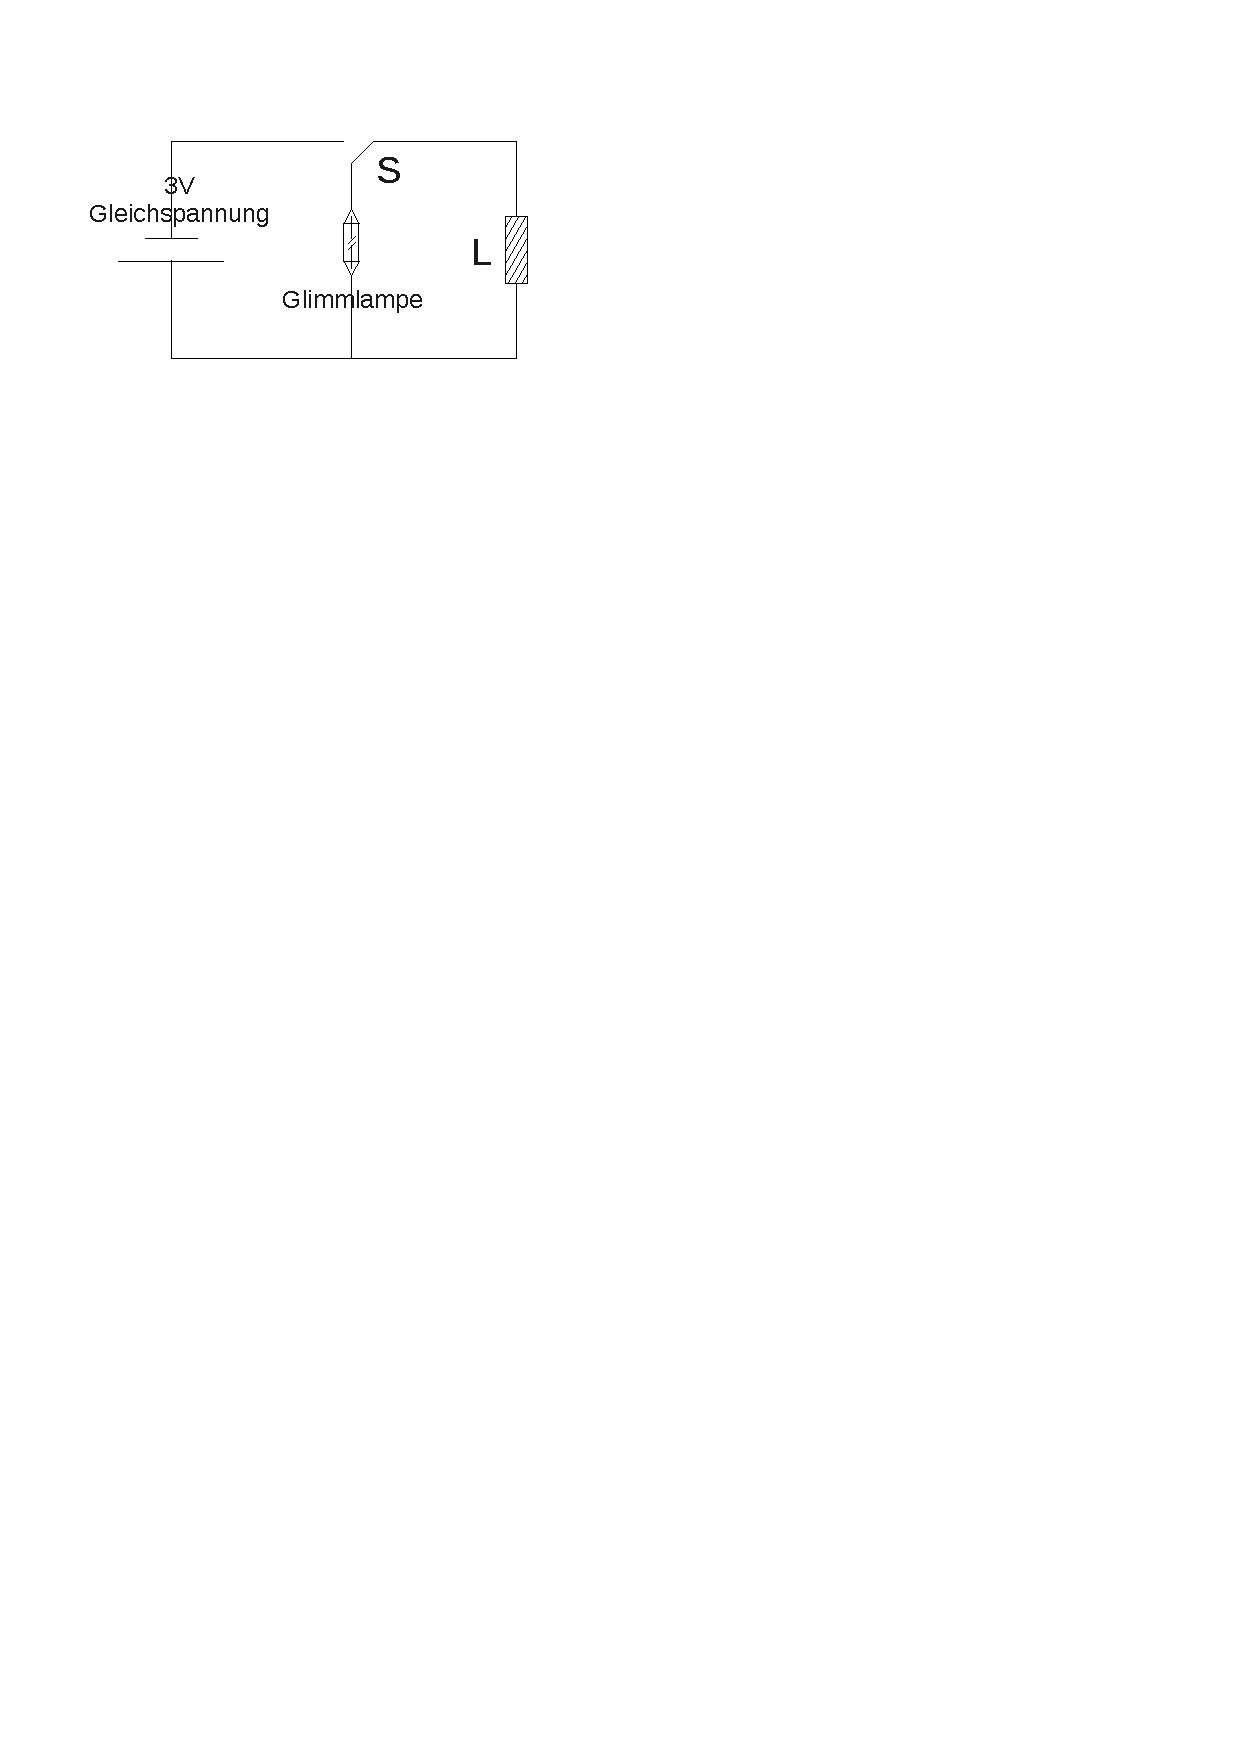
\includegraphics[width=\textwidth]{SelbstinduktionGlimmlampe}
	\caption{Möglicher Schaltkreis mit einer Glimmlampe, die eine hohe Auslösespannung benötigt. \textbf{S} ist ein Schalter der Wahlweise die Gleichspannungsquelle oder die Glimmlampe mit der Spule verbindet.}
	\label{fig:SchaltkreisGlimmlampe}
\end{figure}

Dies lässt sich mit einer parallel zur Spule geschalteten Glimmlampe veranschaulichen, die eine Auslösespannung von circa 60 - 70 Volt besitzt. Sie wird beim Ausschalten des Stromkreises leuchten, auch wenn die Spannung bisher nur wenige Volt betrug.\footnote{"SelbstinduktionGlimmlampeSChaltkreis" von Till Blaha - Eigenes Werk. Lizenziert unter Gemeinfrei}


\section{Energie in Spulen}								\label{sec:EnergieSpule}

%%%%% Physik Kompendium Nr.2 %%%%%
%% 01 -- Energie des Magnetfeldes einer Spule %%


Die Energie, die in Form eines Magnetfeldes in einer Spule gespeichert ist, ist wie folgt zu berechnen:

\begin{equation} \label{eq:EnergieSpule}
	E = \frac{1}{2} L \cdot I^2
\end{equation}

Eine mögliche Herleitung, die eventuell interessant, aber sicher nicht klausurrelevant ist, ist diese. Sie beruht auf der allgemeinen und der elektrischen Leistung ($P = \frac{\mathrm{d}E}{\mathrm{d}t}$ und $P = U \cdot I$) sowie auf der Induktivitätsbeziehung $U = L \cdot \frac{\mathrm{d}I}{\mathrm{d}t} <=> L = U \cdot \frac{\mathrm{d}t}{\mathrm{d}I}$:

\begin{align*}
\begin{split}
	P &= U \cdot I = \frac{\mathrm{d}E}{\mathrm{d}t} \\
	\mathrm{d}E &= U \cdot I \cdot \mathrm{d}t \\
	\frac{\mathrm{d}E}{\mathrm{d}I} &= U \cdot \frac{\mathrm{d}t}{\mathrm{d}I} \cdot I \\
	\frac{\mathrm{d}E}{\mathrm{d}I} &= L \cdot I \\
	E &= \int L \cdot I \ \mathrm{d}I \\
	E &= \frac{1}{2}L \cdot I^2
\end{split}
\end{align*}


\section{Induktion im Alltag}							\label{sec:Alltag}

%%%%% Physik Kompendium Nr.2 %%%%%
%% 03 -- Alltägliche Anwendung der Induktion %%


\subsection{Wirbelstrombremse}

\subsubsection{Funktionsprinzip}
% Cue for review Strom vs Spannung
In einer Wirbelstrombremse induziert ein magnetisches Feld einen Strom in einen, sich durch dieses Feld bewegenden, ferromagnetischen Körper, der wiederum in diesem Körper einen Wirbelstrom bildet. Dieser baut ein Magnetfeld auf, welches, gemäß Lenz'scher Regel, in die entgegengesetzt Richtung zeigt. Damit ziehen sich das sogenannte Bremsschwert und der induzierende Magnet an.

Die Wirkung der Bremse ist proportional abhängig von der Fläche, Induktivität und Geschwindigkeit des Schwertes sowie von der Flussdichte des Magnetfeldes.


\paragraph{Merkmale}

\begin{itemize}

	\item Geschwindigkeitsabhängig
	
Da in der Formel für die Induktionsspannung ($U_{ind}=-L \cdot \frac{dI}{dt}$) die Zeit für die Änderung der Flussdichte im Nenner steht, ist die Bremswirkung bei höheren Geschwindigkeiten höher, Gesetzt dem Fall, dass sich die Fläche des Bremsschwertes und die Stromstärke nicht ändert.

\end{itemize}


\paragraph{Vorteile}

\begin{itemize}
	\item Verschleiß- und Wartungsfreiheit
	
Da bei einer Wirbelstrombremse keine Teile aufeinander Schleifen, ist diese weitgehend frei von Verschleiß und auch deutlich Wartungsfreundlicher.

Lediglich eine zu hohe Hitzeentwicklung sollte verhindert werden.

	\item Ausfallsicherheit
	
Während herkömmliche Bremsen abhängig von Hydraulik oder Kabelzügen etc. sind, funktionieren Wirbelstrombremsen allein mit Strom, oder, wenn sie mit Permanentmagneten statt Elektromagneten ausgestattet sind, komplett Ausfallsicher.

\end{itemize}

\paragraph{Nachteile}

\begin{itemize}

	\item Kein vollständiges Abbremsen möglich
	
Aufgrund der Abhängigkeit von der Geschwindigkeit, ist es theoretisch nicht möglich, allein mit einer Wirbelstrombremse einen Gegenstand zum Stillstand zu bringen.

\end{itemize}


\subsubsection{Typische Anwendungen}

Die Wirbelstrombremse findet als klassische Bremse für Fahrzeuge häufig Anwendung in Achterbahnen und Trams, da diese oft mit einer vorhersehbaren Geschwindigkeit unterwegs sind, und daher die Bremswirkung genau berechnet werden kann. Dies ist für die Wirbelstrombremse recht wichtig, da, wie schon erwähnt, die Bremswirkung von der Geschwindigkeit abhängig ist.

In Freefalltowern werden Wirbelstrombremsen mit Permanentmagneten eingesetzt, um Sicherheit auch bei einem plötzlichen Stromausfall zu gewährleisten.

In LKWs unterstützten sie manchmal die herkömmliche Bremse.

In Hometrainern hält eine induktionsbasierte Bremse das Gerät Wartungsfreier und leiser.


\subsection{Induktionsherd}

\subsubsection{Funktionsprinzip}

Unter der Herdplatte sitzt eine Spule, durch die ein hochfrequenter Wechselstrom fließt. Dadurch entsteht ein sich ständig änderndes Magnetfeld, welches dann ständig einen Strom in den Boden des Topfes induziert und in diesem für Wärmeentwicklung sorgt.

Die Stärke ist in der Regel proportional Abhängig von der gewählten Frequenz und Stärke des Magnetfeldes, sowie des Materials des Topfes.


\paragraph{Vorteile}

\begin{itemize}
	\item Bessere Regelbarkeit und Ansprache
	
Die Wärmeentwicklung lässt sich sehr gut Steuern und der Herd spricht sehr schnell an, was ihn optimal für große Küchen macht, in denen dies erforderlich ist.

	\item Geringe Wärmeentwicklung auf der Herdplatte
	
Da die Hitze sich erst im Topf entwickelt, ist die Herdplatte deutlich weniger heiß als bei einem herkömmlichen Herd, was vor Verbrennungen schützt.

	\item Effizienz
	
Ein Induktionsherd ist deutlich effizienter als ein herkömmlicher Elektroherd, da keine Energie in die Aufheizung der Platte gesteckt werden muss.
\end{itemize}



\paragraph{Nachteile}

\begin{itemize}

	\item Neue Töpfe

Natürlich benötigen die Töpfe bzw. Pfannen einen ferromagnetischen Boden, was bei herkömmlichen Töpfen häufig nicht gegeben ist. Daher muss eventuell viel Geld für ein neues Topf-/Pfannenset ausgegeben werden.
\end{itemize}



\chapter{Wechselstrom} \label{ch:Wechselstrom}
\section{Erläuterungen zum Wechselstromkreis}				\label{sec:Erlaeuterungen}

\subsection{Grundlegende Begriffe}		\label{subsec:ErlaeuterungenGrundlegend}

\subsubsection{Wechselstrom}

Mit Wechselstrom bezeichnet man einen Strom, der nicht nur von einem Punkt zum anderen fließt, sondern mit einer Frequenz die Fließrichtung wechselt. Interessant ist, dass obwohl unter dem Strich keine Elektronen vollständig \glqq überlaufen\grqq{} , trotzdem Energie umgesetzt werden kann.

Im Idealfall, von dem auch bei allen folgenden Betrachtungen ausgegangen wird, weist die Spannungs- und Stromkurve, über der Zeit, den Verlauf einer Sinuskurve auf.


\subsubsection{Amplitude}

Die Amplitude ist die maximale Auslenkung der Spannung oder der Stromstärke, also der Scheitelwert (y-Wert). Oft mit $\hat{U}$ bzw. $\hat{I}$, $U_{0}$ bzw. $I_{0}$ oder $U_{max}$ bzw. $I_{max}$ angegeben.


\subsubsection{Periode}

Dauer, bis eine volle Sinuskurve der Spannung vollendet ist, also die Spannung wieder den Nullpunkt aus der selben Richtung passiert, wie beim ersten Durchlauf.

Bei einem Wechselstromgenerator (siehe \referenz{sec:Generator}) ist dies die Dauer, bis sich die Spule einmal um 360\degree{} gedreht hat.


\subsubsection{Frequenz}

Bezeichnet die Anzahl Perioden pro Zeiteinheit. 

\noindent Aus der Periodendauer ist die Formel $f=\frac{1}{T}$, wobei $T$ die Periodendauer, die Zeit für eine Periode, ist. Die Einheit ist $Hz$ (spricht: \glqq Hertz\grqq), also $\frac{1}{s}$.



\subsubsection{Winkelgeschwindigkeit}

Die Länge einer Periode einer Sinuskurve kann man auch mit $360\degree$ ausdrücken, was praktisch ist, wenn man keine absolute Zeitspanne benötigt, sondern mit Anteilen bzw. Abschnitten rechnet oder argumentiert. Obwohl sich $360\degree$ recht gut teilen lässt, rechnet man in der Physik meistens im Bogenmaß. $360\degree$ entsprechen dann $2\pi$.

\begin{NiceToKnow}
Umrechnung des Winkels $\alpha$ von Grad ins Bogenmaß: $\frac{\alpha}{180} \cdot \pi$
\end{NiceToKnow}

Die Winkelgeschwindigkeit gibt nun an, wie groß der Abschnitt ist, der pro Zeit absolviert wird:

\begin{equation}	\label{eq:Winkelgeschwindigkeit}
	\omega = \frac{2\pi}{T} = 2\pi f
\end{equation}

\begin{Wichtig}
Daran Denken, dass der Taschenrechner bei Winkelfunktionen ($\sin$, $\cos$ usw.) und Rechnung im Bogenmaß auf \glqq Radiant\grqq{} stehen muss. Beim Casio-fx991xx [SHIFT] + [SET UP] + [4] drücken. [SHIFT] + [SET UP] + [4] stellt wieder auf Gradmaß um.
\end{Wichtig}


\subsection{Weitere Begriffe}	\label{subsec:ErlaeuterungenWeitere}

\subsubsection{Effektive Spannung}

Diese beschreibt die durchschnittliche Spannung im Wechselstromkreis, die zum weiteren Rechnen wie eine Spannung im Gleichstromkreis behandelt werden kann.

Für eine Sinuskurve lässt sie sich wie folgt, in Abhängigkeit der maximalen Spannung, berechnen:

\begin{equation}	\label{eq:EffektiveSpannung}
	U_{eff}=\frac{\hat{U}}{\sqrt{2}}
\end{equation}


\subsubsection{Effektive Stromstärke}

Diese beschreibt die durchschnittliche Stromstärke im Wechselstromkreis, die zum weiteren Rechnen wie eine Stromstärke im Gleichstromkreis behandelt werden kann.

Für eine Sinuskurve lässt sie sich wie folgt, in Abhängigkeit der maximalen Stromstärke, berechnen:

\begin{equation}	\label{eq:EffektiveStromstaerke}
	I_{eff}=\frac{\hat{I}}{\sqrt{2}}
\end{equation}


\subsubsection{Phasenverschiebung}

Eine Phasenverschiebung ist die Verschiebung einer Kurve entlang der x-Achsen, typischerweise die Verschiebung der Kurve des Stroms relativ zur Kurve der Spannung. Sie wird in Grad oder im Bogenmaß angegeben. Siehe folgende Abbildung\endnote{\glqq Phasenverschiebung Spannung vor Strom\grqq{} by Till Blaha - Eigenes Werk. Lizenziert unter Gemeinfrei.}:


\begin{figure}[H]
	\centering
	\begin{comment} Gnuplot: './xpitics.p'
set xlabel "t"
set ylabel "I, U"
set output "plot_spannungen_vor_strom.png"
plot cos(x)*0.7 title "Strom" ls 1, sin(x) title "Spannung" ls 3
	\end{comment}
	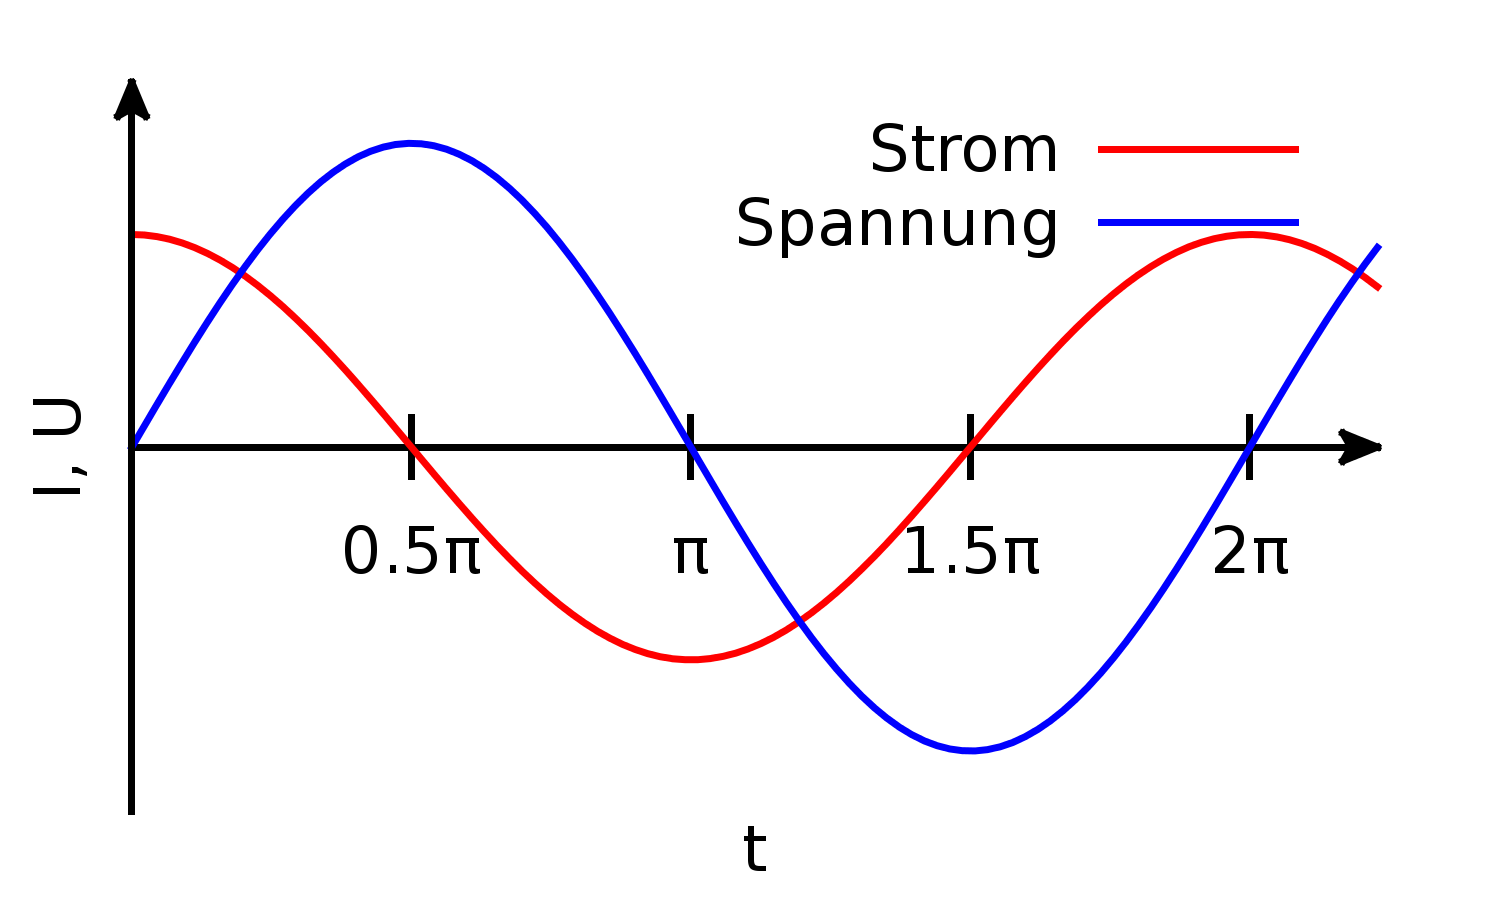
\includegraphics[width=0.7\textwidth]{plot_spannungen_vor_strom}
	\caption{\glqq Der Strom hinkt der Spannung um $\frac{\pi}{2}$ bzw. 90\degree{} hinterher.\grqq }
\end{figure}



\subsubsection{Impedanz}

Die Impedanz $Z$ ist der effektive Gesamtwiderstand im Wechselstromkreis. Die Impedanz trägt wie der Ohm'sche Widerstand die Einheit \emph{Ohm} mit Zeichen $\Omega$. Sie ist der Quotient aus der Spannung und der Stromstärke:

\begin{equation}		\label{eq:Impedanz}
	Z = \frac{U_{eff}}{I_{eff}}
	  = \frac{\hat{U}}{\hat{I}}
\end{equation}


\subsubsection{Kapazitiver Widerstand}

Für den kapazitiven Widerstand $X_C$, der von Kondensatoren im Wechselstromkreis ausgeht, siehe \referenz{subsec:KapazitiverWiderstand}.


\subsubsection{Induktiver Widerstand}

Für den induktiven Widerstand $X_L$, der von Spulen im Wechselstromkreis ausgeht, siehe \referenz{subsec:InduktiverWiderstand}.









\section{Prinzip des Wechselstromgenerators}				\label{sec:Generator}

\subsection{Funktionsprinzip}

Eine Spule, oder der Anschaulichkeit halber, eine Leiterschleife, befindet sich in einem magnetischen Feld (Siehe Abbildung).\footnote{Abbildung von LeiFi Physik: \url{http://www.leifiphysik.de/sites/default/files/medien/generator02_elmagnetindukt_ver.gif}}

\begin{figure}[h!]
	\centering
	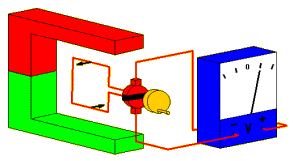
\includegraphics[width=0.6\textwidth]{GeneratorSchema}
	\caption{Schema eines Wechselstromgenerators mit Kommutator} 
\end{figure}


Die Leiterschleife wird angedreht und der sich in der Grafik oben befindende Teil der Schleife bewegt sich senkrecht zu den Feldlinien des Magnetfeldes. Somit wirkt auf die Teilchen die Lorentzkraft, gemäß Linker-Hand-Regel (Siehe \referenz{sec:lorentzkraft}). Im Beispiel ist der Plus-Pol am oberen Ende und der Minus-Pol am unteren Ende.

Wenn sich die Schleife nun um 90\degree{} gedreht hat, bewegen sich beide Pole kurzzeitig parallel zu den Feldlinien; die Elektronen in der Schleife werden nicht mehr beeinflusst und es liegt keine Spannung mehr an. Der sinusförmige Spannungsgraph resultiert aus der Bewegung dazwischen.

Nach weiteren 90\degree{} ist das ursprünglich obige Stück Schleife unten und nun der Minus-Pol. Das ist der Grund für die negativen Passagen der Spannungskurve.


\subsubsection{Kommutator}

Ein Kommutator, wie in der Abbildung, kehrt die Polarität der Leiterschleifenteile bei jeder halben Umdrehung um, sodass es nie eine negative Spannung gibt. Der schwarze Teil ist ein Isolator und die Backen, die oben und unten liegen, schleifen über Bürsten am sich drehenden Kommutator.

Die Spannungskurve\footnote{„Betrag von sinx“ von Till Blaha - Eigenes Werk. Lizenziert unter Gemeinfrei} ist dann der Betrag: $|\sin x|$:

\begin{figure}[h!]
	\centering
	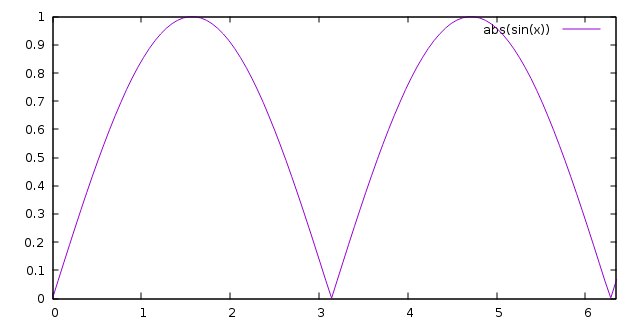
\includegraphics[width=0.7\textwidth]{Betragsinx}
	\caption{Ideale Spannungskurve mit einem Kommutator.} 
\end{figure}


\subsection{Induktionsspannung bestimmen}

Um die maximale Spannung (Amplitude), zu bestimmen, muss die Feldstärke des Magnetfeldes, die Windungszahl, Fläche und Induktivität der Spule sowie die Drehfrequenz bekannt sein. Die Gleichung ist analog zur generellen Induktionsspannung (Siehe \gleichungsreferenz{eq:InduGe}) $U_{ind} = -N \frac{d(B \cdot A)}{dt}$:

\begin{equation}	\label{eq:hatU}
	\hat{U} = NBA \cdot \omega
\end{equation}

\noindent Daraus folgt für einen beliebigen Zeitpunkt:

\begin{align}		\label{eq:hatUbeliebig}
\begin{split}
	U(t) &= \hat{U} \cdot sin(\omega \cdot t) \\
	U(t) &= NBA \cdot \omega \cdot sin(\omega \cdot t)
\end{split}
\end{align}






\section{Widerstände im Wechselstromkreis}					\label{sec:Widerstaende}

Während es im Gleichstromkreis nur den Ohm'schen Widerstand gibt, verfügt man im Wechselstromkreis über drei Typen.

Die restlichen zwei Arten, der kapazitive und der induktive Widerstand, generieren Phasenverschiebungen, welche in sogenannten Blindwiderständen resultieren.


\subsection{Ohm'sche Widerstände}		\label{subsec:OhmscherWiderstand}

Wenn in einem Wechselstromkreis nur Ohm'sche Widerstände verbaut sind, ist die Impedanz $Z$, also der Gesamtwiderstand des Kreises, gleich der Summe der Widerstände.

Das bedeutet, er verursacht keine Phasenverschiebung und kann wie ein Widerstand im Gleichstromkreises behandelt werden.


\subsection{Kapazitive Widerstände}		\label{subsec:KapazitiverWiderstand}

Kondensatoren verursachen kapazitive Widerstände. Da Kondensatoren keinen Durchfluss erlauben, wäre ihr Widerstand im Gleichstromkreis unendlich. Im Wechselstromkreis verursacht er aber eine Phasenverschiebung des Stromes, welcher dann um 90\degree{} der Spannung vorauseilt.

Beim Wechselstrom schwingen die elektrischen Ladungen nämlich hin und her. Ein Kondensator im Wechselstromkreis wird also abwechselnd geladen, wieder entladen und dann anders gepolt geladen. Die Spannung zwischen den Kondensatorplatten baut sich während den Ladevorgängen mit der Zeit auf und erreicht ihr Maximum dann, wenn der Kondensator vollständig aufgeladen und der Stromfluss zum Erliegen gekommen ist. Bei den Entladevorgängen sind die Verhältnisse umgekehrt: Die Stromstärke ist dann am größten, wenn der Kondensator vollständig entladen ist.\endnote{Paragraph von: \url{http://files.sma.de/dl/10040/BLINDLEISTUNG-ADE094210.pdf}}

\glqq Der Strom eilt der Spannung voraus.\grqq

\vspace{11pt}

\noindent Dieser sogenannte \glqq Kapazitive Blindwiderstand\grqq{} ist antiproportional abhängig von der Kapazität des Kondensators, da der Anteil der Zeit, in der der Kondensator vollständig oder annähern vollständig geladen ist, größer ist, da eine kleinere Kapazität dafür sorgt, dass mit weniger Ladung schon eine hohe Spannung erreicht wird (Siehe: \gleichungsreferenz{eq:kapazitaet}). Damit ist der Stromfluss bei einer kleinen Kapazität stärker gehemmt als bei einer großen Kapazität. 

$X_C$ ist außerdem antiproportional abhängig von der Winkelgeschwindigkeit (Siehe: \referenz{subsec:ErlaeuterungenGrundlegend}), da bei einer raschen Umpolung der Wechselspannung (also $f$ und demnach auch $\omega$ recht groß) die Zeit in der der Stromfluss durch einen vollständig geladenen Kondensator gehemmt ist, kleiner wird.

Daraus folgt:

\begin{equation}	\label{eq:KapazitiverWiderstand}
	X_C = \frac{1}{\omega \cdot C}
\end{equation}


\subsection{Induktive Widerstände}		\label{subsec:InduktiverWiderstand}

Eine Spule leitet Gleichstrom wie ein normaler Draht. Nur beim Ein- und Ausschalten gibt es jeweils eine Zeitverzögerung im Stromfluss, die durch die Selbstinduktion (Siehe \referenz{sec:Selbstinduktion}) während des Auf- und Abbaus des Magnetfeldes verursacht wird. Unter Wechselstrombedingungen kommt es bei jedem Wechsel der Stromrichtung zu diesen Verzögerungen. Dies resultiert in einer Phasenverschiebung des Stromes um -90\degree .\endnote{Paragraph von: \url{http://files.sma.de/dl/10040/BLINDLEISTUNG-ADE094210.pdf}}

\glqq Die Spannung eilt dem Strom voraus.\grqq

\vspace{11pt}

Der \glqq Induktive Widerstand\grqq{} ist proportional abhängig von der Induktivität der Spule, da ein höheres Vermögen, bei jedem Umpolen Spannung in sich selbst zu induzieren, sich in einer stärkeren Hemmung des Stromflusses äußert.

Der induktive Widerstand ist ebenfalls proportional zur Winkelgeschwindigkeit, da bei einer höheren Winkelgeschwindigkeit öfters umgepolt wird und der Prozess der Selbstinduktion häufiger den Stromfluss hemmt und die Zeit in der der Strom ungehindert fließen kann (nach vollständigem Aufbau des Magnetfeldes) kürzer wird.

Daraus folgt:

\begin{equation}	\label{eq:InduktiverWiderstand}
	X_L = \omega \cdot  L
\end{equation}


\subsection{Auswirkungen von Blindwiderständen auf die Stromstärke} \label{subsec:AuswirkungenWiderstand}

Man kann die Gleichung für die Impedanz (Gleichung \ref{eq:Impedanz} auf Seite \pageref{eq:Impedanz}) nach $I$ umstellen, um sich zu verdeutlichen, dass eine erhöhte Impedanz, in welcher der Blindwiderstand steckt, eine niedrigere Stromstärke zur Folge hat, genau wie der Ohm'sche Widerstand im Wechselstromkreis:

\begin{equation}	\label{eq:ImitZ}
	I_{eff}=\frac{U_{eff}}{Z}
\end{equation}


\subsection{Frequenzabhängigkeit}	\label{subsec:Frequenzabhaengigkeit}

Die Größe der Blindwiderstände ist sowohl beim Kondensator als auch bei der Spule abhängig von der Frequenz des Wechselstromes (diese Steckt im $\omega$).

Der kapazitive Blindwiderstand ist antiproportional abhängig (Siehe Gleichung \ref{eq:KapazitiverWiderstand}) von der Frequenz, was bedeutet: \glqq Ein Kondensator erhöht die Impedanz, je niedriger die Frequenz ist.\grqq{} Man sagt auch \glqq High-Pass-Filter\grqq{} oder \glqq Low-Cut-Filter\grqq .

Der induktive Blindwiderstand ist proportional abhängig (Siehe Gleichung \ref{eq:InduktiverWiderstand}) von der Frequenz, was bedeutet: \glqq Eine Spule erhöht die Impedanz, je höher die Frequenz ist.\grqq{} Man sagt auch \glqq Low-Pass-Filter\grqq oder \glqq High-Cut-Filter\grqq .

Diese Eigenschaften macht man sich in der Audiotechnik bei Frequenzweichen oder Equalisern zu Nutze. Siehe auch \referenz{subsec:Siebkreis}.



\subsection{Zeigerdiagramm}	\label{subsec:WiderstaendeZeigerdiagram}

Die Impedanz ist auch berechenbar, wenn der Ohm'sche Widerstand und der Blindwiderstand bekannt sind. Bevor Gesetze betrachtet werden, ist das Zeigerdiagramm\endnote{"Zeigerdiagramm für Widerstände" by Till Blaha - Mit Gnuplot selbst erstellt. Lizenziert unter Gemeinfrei.} eine gute Veranschaulichung für die Beziehungen und den Phasenverschiebungswinkel.

\begin{figure}[h!]
	\centering
	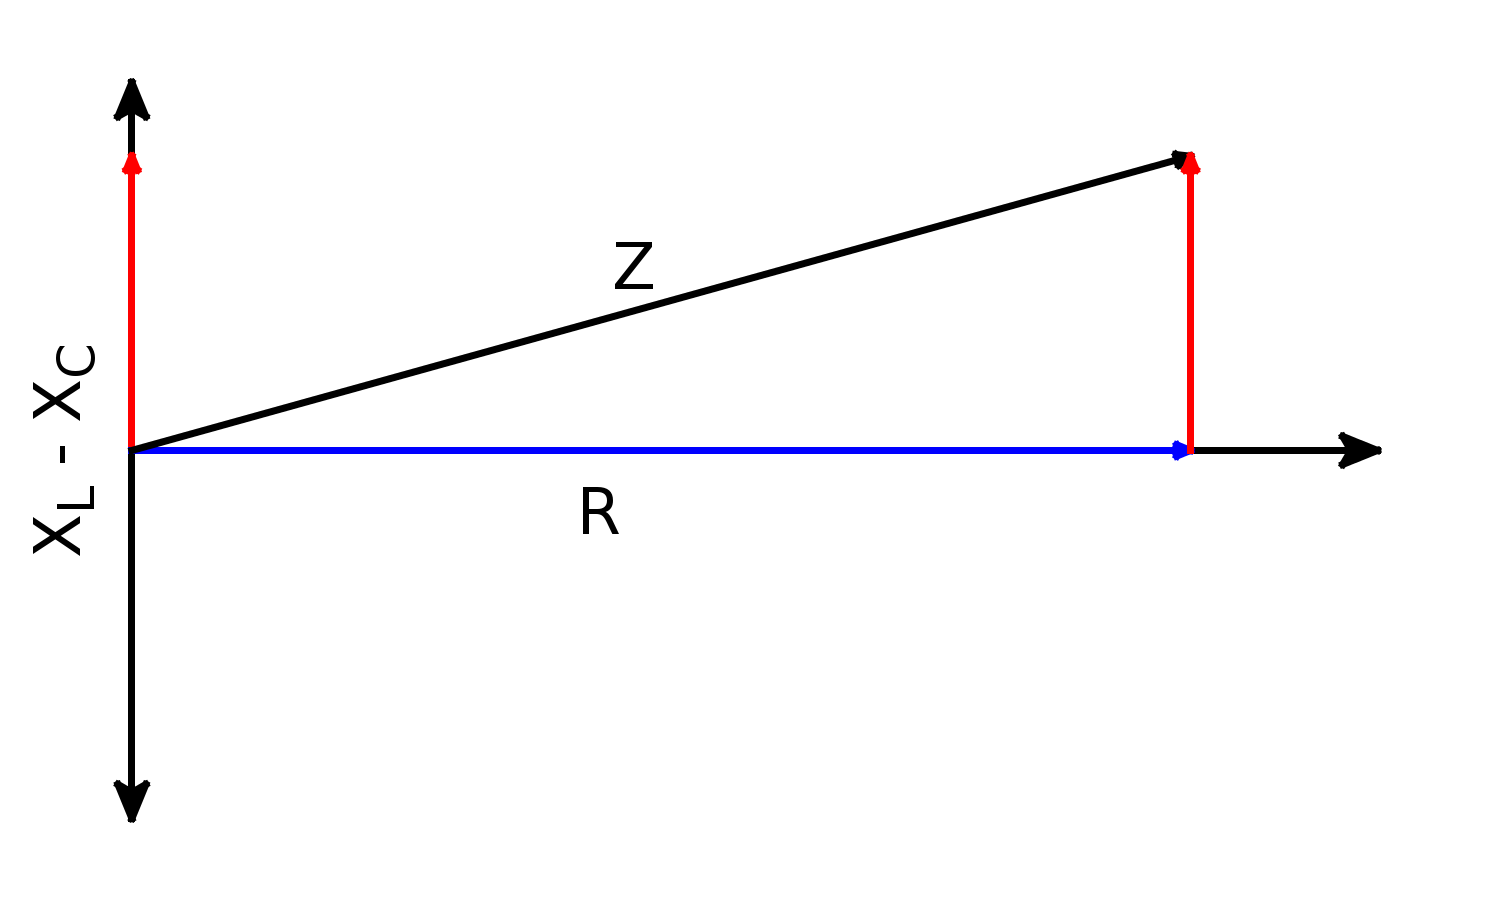
\includegraphics[width=0.8\textwidth]{plot_zeigerdiagramm}
	\begin{comment} Gnuplot:
set ylabel "X_L - X_C"
set label "R" at 2.5,-0.2
set label "Z" at 2.7,0.6
set arrow from graph 0,0.5 to graph 0,0.9 size screen 0.01,22,60 filled ls 1 front
set arrow from graph 0,0.5 to graph 0.85,0.5 size screen 0.01,22,60 filled ls 3 front
set arrow from graph 0,0.5 to graph 0.85,0.9 size screen 0.01,22,60 filled ls 2 front
set arrow from graph 0.85,0.5 to graph 0.85,0.9 size screen 0.01,22,60 filled ls 1 front
unset key
set output "plot_zeigerdiagramm.png"
plot 100
	\end{comment}
	\caption{Zeigerdiagramm mit Widerständen: Blau: Ohm'scher Widerstand, Rot: Blindwiderstand, Schwarz: Impedanz, Der Phasenverschiebungswinkel ist der Winkel zwischen der Impedanz (Hypothenuse) und dem Ohm'schen Widerstand (Kathete)}
\end{figure}


Das Diagramm veranschaulicht den Zusammenhang zwischen dem Verhältnis des Blindwiderstandes und dem Ohm'schen Widerstand. Dieses Verhältnis ist nämlich immer gleich dem Tangens des Winkels $\varphi$.

\begin{Anmerkung}
Sollten in einem Schaltkreis beide Blindwiderstände (eine Spule und ein Kondensator) verbaut sein, muss für die Differenz für $X_{Ges}$ angenommen werden, da beide eine Phasenverschiebung in die jeweils andere Richtung verursachen.
\end{Anmerkung}

\noindent Für $X_{Ges}$ gilt dann:

\begin{equation}	\label{eq:BlindwiderstandSumme}
	X_{ges} = X_L - X_C = \omega \cdot L - \frac{1}{\omega \cdot C}
\end{equation}



\subsection{Gesetze}	\label{subsec:WiderstaendeGesetzte}

Nun ist auch die Betrachtung der Gesetze, angelehnt an diese Darstellungsform, deutlich einfacher.


Für die Impedanz können nun, zusätzlich zur \gleichungsreferenz{eq:Impedanz}, noch andere Betrachtungen gefunden werden:

In Abhängigkeit von $X$ und $R$ mit dem Satz des Pythagoras:

\begin{equation}	\label{eq:ImepdanzXR}
	Z = \sqrt{X^2 + R^2}
\end{equation}


\noindent In Abhängigkeit von $X$ und $\varphi$ mit weiteren Winkelbeziehungen im rechtwinkligen Dreieck:

\begin{equation}	\label{eq:ImepdanzXphi}
	Z = \frac{X}{\sin\varphi}
\end{equation}


\noindent In Abhängigkeit von $R$ und $\varphi$:

\begin{equation}	\label{eq:ImepdanzRphi}
	Z = \frac{R}{\cos\varphi}
\end{equation}


\section{Schwingkreise}										\label{sec:Schwingkreise}

Schwingkreise sind Schaltkreise, die aus den zwei Wechselstromwiderständen Spule und Kondensator sowie (in der Theorie) aus einem Ohm'schen Widerstand bestehen. Daher nennt man sie auch LC- oder LCR-Schaltungen. In der Praxis könnte auf einen Ohm'schen Widerstand verzichtet werden, da eine reelle Spule immer auch einen Ohm'schen Widerstand besitzt, denn sie besteht aus Draht. 

Diese Stromkreise haben in der Wechselstromumgebung frequenzabhängige Eigenschaften (Siehe \referenz{subsec:Frequenzabhaengigkeit}), sowie eine Resonanzfrequenz, bei der sich die Größe der beiden Wechselstromwiderstände die Waage halten und der Blindwiderstand folglich $0$ ist (Siehe \gleichungsreferenz{eq:BlindwiderstandSumme}).

\subsection{Natürliche Schwingkreis}

Der Schwingkreis\endnote{„SchwingkreisSchaltung“ von Till Blaha - Eigenes Werk. Lizenziert unter Gemeinfrei} ist ein essentieller Bestandteil von Oszillatoren, also Schwingungsgeneratoren. 

\begin{figure}[h!]
	\centering
	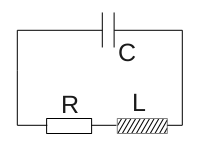
\includegraphics[width=0.5\textwidth]{Schwingkreis}
	\caption{Diagramm des Schwingkreises}
\end{figure}

Im Stromkreis sind alle Bauteile in Reihe geschaltet und es gibt keine externe Spannungsquelle. Jedoch ist der Kondensator zu Anfang geladen; er trägt anfangs die gesamte Energie des Aufbaus.

\begin{figure}[h!]
	\centering
	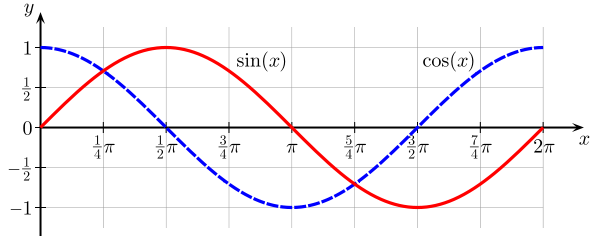
\includegraphics[width=0.8\textwidth]{SchwingkreisGraph}
	\caption{Spannung (blau) und Stromstärke (rot) in einem Schwingkreis über der Zeit}
\end{figure}

Sobald der Kreis, bspw. über einen Schalter, geschlossen wurde, entlädt sich der Kondensator; die Spannung fällt. Durch die Selbstinduktion an der Spule steigt die Stromstärke jedoch langsam an, welche ohne diesen induktiven Widerstand sofort nach dem schließen des Schalters auf ihrem Maximum gewesen wäre.

Auch wenn der Kondensator vollständig entladen ist (Stelle $\frac{1}{2}\pi$ im Diagramm\endnote{„Sine cosine one period“ von Geek3 - Eigenes Werk. Lizenziert unter CC BY 3.0 über Wikimedia Commons - \url{https://commons.wikimedia.org/wiki/File:Sine_cosine_one_period.svg}}), also die Spannung $0V$ beträgt, ist immer noch eine Stromstärke messbar, da der Ladungsfluss durch die Selbstinduktion in der Spule verzögert ist. Allerdings ist der Verlauf der Stromstärke fallend, da keine weitere Ladung mehr in die Spule fließt (der Kondensator ist entladen). An der Stelle $\frac{1}{2}\pi$ trägt der Kondensator keine Ladung und die maximale Stromstärke ist erreicht, was bedeutet, dass zu diesem Zeitpunkt die gesamte Energie der Schaltung im Magnetfeld der Spule gespeichert ist.

Im Abschnitt zwischen $\frac{1}{2}\pi$ und $\pi$ ist die Spannung negativ, das heißt die Kondensatorplatten wurden und werden mit anderer Polung als am Anfang des Versuches geladen. Trotzdem fließen immer noch weitere Ladungen auf die Kondensatorplatten, da der Stromfluss durch die Spule verzögert wurde. Sobald der Kondensator vollständig geladen wurde ($\pi$), fließt kein Strom mehr (Stromstärke ist $0A$), das heißt, es gibt kein Magnetfeld mehr und die gesamte Energie ist, wie zu Beginn, im Kondensator gespeichert.

Dieser Vorgang wiederholt sich periodisch, bis die Ladungen durch den Verbraucher (in diesem Fall den Ohm'schen Widerstand) verbraucht wurden, in diesem Fall in Wärme umgewandelt wurden.

\subsubsection{Resonanzfrequenz}

Die Resonanzfrequenz ist die Frequenz, bei der die Impedanz so klein wie möglich ist, das heißt, die angestrebte Frequenz, die oszilliert wird.

Um eine kleinstmögliche Impedanz zu erreichen, muss der Blindwiderstand $0$ sein, woraus folgt, der reelle Teil des Gesamtwiderstands (der Ohm'sche Widerstand) die gesamte Impedanz ausmacht. Aus Gleichung \ref{eq:BlindwiderstandSumme} abgeleitet, gilt:

\begin{align}	\label{eq:ResonanzfrequenzSchwingkreis}
\begin{split}
	X_L - X_C &= 0 \\
	X_L &= X_C \\
	\omega \cdot L &= \frac{1}{\omega \cdot C} \\
	\omega ^2 &= \frac{1}{C \cdot L} \\
	\omega &= \frac{1}{\sqrt{C L}} \\	
	f &= \frac{1}{2 \pi \cdot \sqrt{C L}} \\
\end{split}
\end{align}


\subsection{Siebkreis} \label{subsec:Siebkreis}

Der Siebkreis (manchmal auch LCR-Schaltung oder Reihenschwingkreis genannt) ist eine bekannte technische Anwendung, deren Aufgabe es ist, aus einem bestehenden Signal (angedeutet im Diagramm\endnote{„SiebkreisSchaltung“ von Till Blaha - Eigenes Werk. Lizenziert unter Gemeinfrei}) einen bestimmten Frequenzbereich \glqq herauszufiltern\grqq , will sagen, dort die geringste Impedanz und folglich die höchste Stromstärke aufzuweisen.

\begin{figure}[h!]
	\centering
	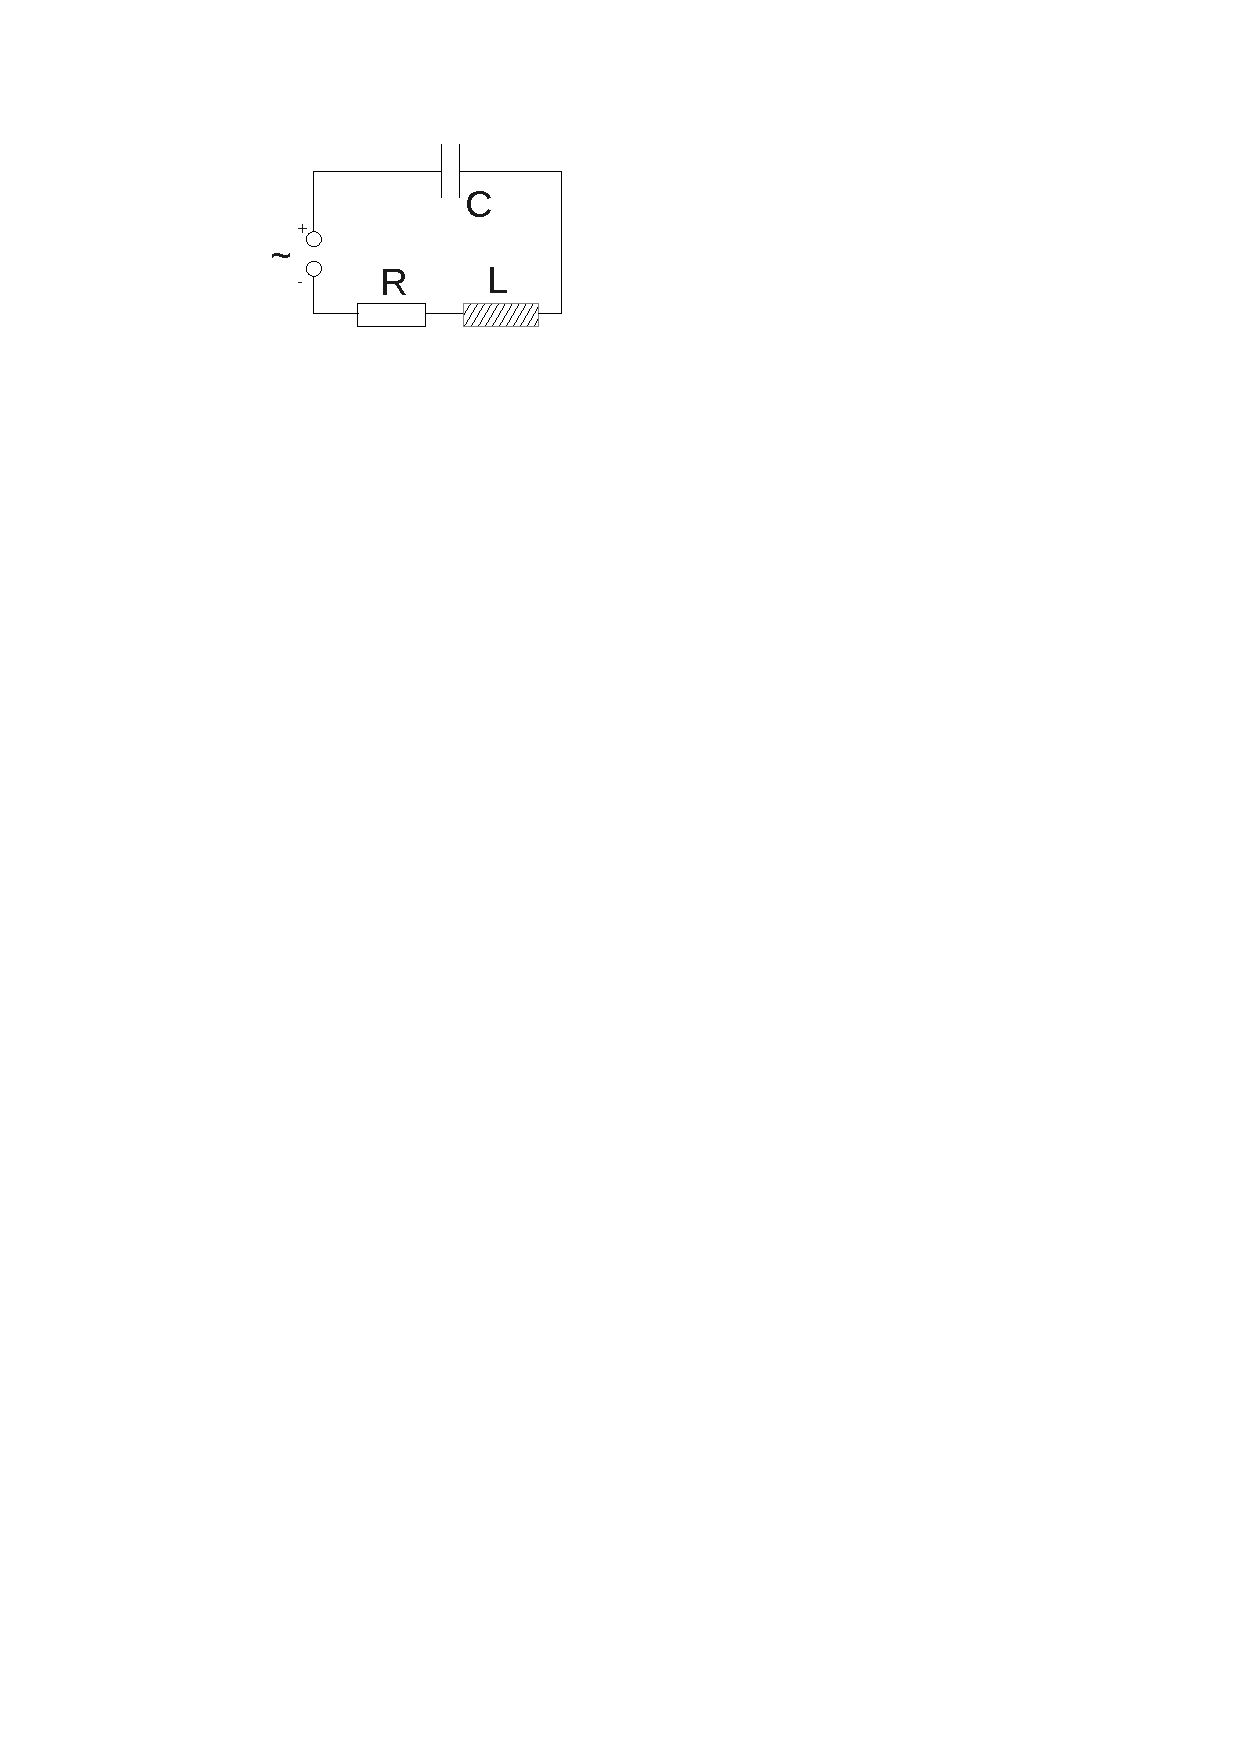
\includegraphics[width=0.5\textwidth]{Siebkreis}
	\caption{Diagramm eines Siebkreises}
\end{figure}

Der Kondensator \glqq schneidet\grqq{} die hohen Frequenzen \glqq ab\grqq , die Spule die tiefen. Siehe Sektionen \referenz{subsec:Frequenzabhaengigkeit} und \referenz{subsec:AuswirkungenWiderstand} für weitere Erläuterungen.

Der Frequenzbereich, also dessen Lage im Spektrum und dessen Breite, wird durch die Daten der Bauteile bestimmt.


\subsubsection{Resonanzfrequenz}

Die Resonanzfrequenz, also die Frequenz mit dem geringsten Gesamtwiderstand, lässt sich genauso berechnen wie beim Schwingkreis:

\begin{align}	\label{eq:ResonanzfrequenzSiebkreis}
\begin{split}
	X_L - X_C &= 0 \\
	f &= \frac{1}{2 \pi \cdot \sqrt{C \cdot L}}
\end{split}
\end{align}

Ist die Frequenz des Wechselstroms nun höher als die Resonanzfrequenz ist die Impedanz höher, da der induktive Widerstand größer wird; bei niedrigerer Frequenz nimmt der kapazitive Widerstand zu. Dieses Diagramm\endnote{„SiebkreisGraph“ von Till Blaha - Eigenes Werk. Lizenziert unter Gemeinfrei} zeigt eine mögliche Stromstärke/Widerstand-über-Frequenz-Kurve:

\begin{figure}[h!]
	\centering
	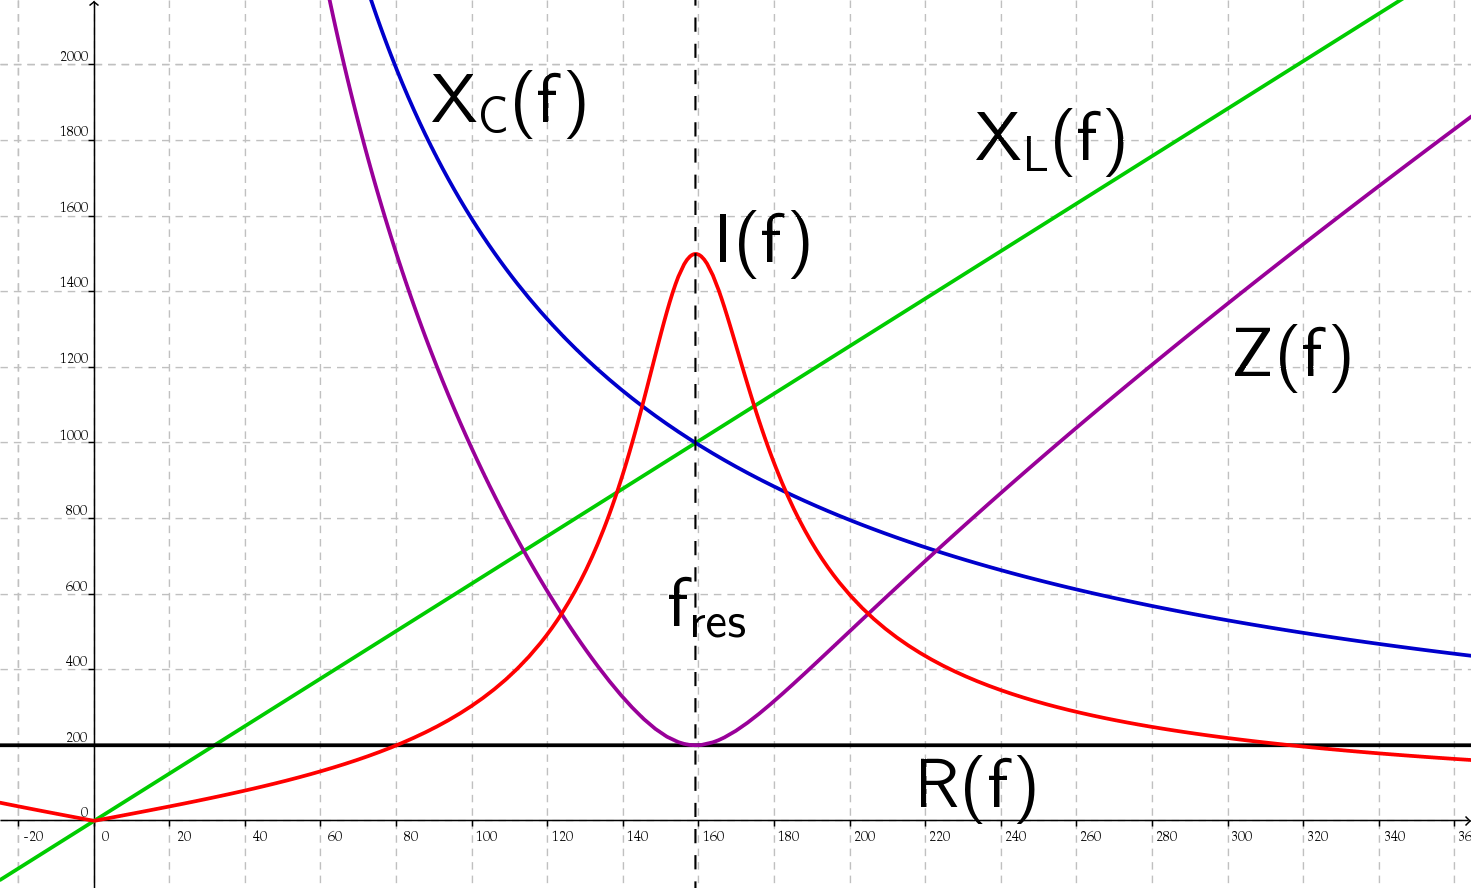
\includegraphics[width=\textwidth]{SiebkreisGraph}
	\caption{Die 3 Widerstände, Impedanz und Stromstärke mit fiktiver y-Skalierung. Frequenz auf der x-Achse. Man beachte die Schnittstelle von $X_L$ und $X_C$ die Gleichzeitig der Tiefpunkt der Impedanz $Z$ und damit der Hochpunkt der Stromstärke $I$ ist.}
\end{figure}







\section[Leistungen im Wechselstromkreis]{Leistungen und deren Auswirkungen im Wechselstromkreis}	\label{sec:Leistungen}

%%%%% Physik Kompendium Nr.2 %%%%%
%% 07 -- Leistungen %%


\subsection{Wirkleistung und Blindleistung}

Auch und vor allem bei der Leistung muss im Wechselstromkreis zwischen Wirk- und Blindleistung unterschieden werden. Die Wirkleistung ist am Ende nutzbar, während die Blindleistung allein die Bauteile belastet und nicht genutzt wird. Das bedeutet, dass es sein kann, dass obwohl ein Stromkreis nur eine bestimmte effektive Wirkleistung umsetzt, aber durch Phasenverschiebungen die Bauteile deutlich stärker belastet werden.


\subsection{Scheinleistung}

Diese ist, analog zur Impedanz (Siehe Sektion \ref{subsec:WiderstaendeZeigerdiagram} auf Seite \pageref{subsec:WiderstaendeZeigerdiagram}), die Hypotenuse eines rechtwinkligen Dreiecks, deren Katheten die Wirkleistung und die Blindleistung sind. Der Winkel $\varphi$ ist ebenfalls der Phasenverschiebungswinkel.


\subsection{Gleichungen}

Die Wirkleistung sowie Blindleistung lassen sich auf viele Arten bestimmen. \\
\vspace{11pt}
Abhängig von der effektiven Spannung und der effektiven Stromstärke:

\begin{align}		\label{eq:ScheinleistungUI}
	P_{Schein} &= U_{eff} \cdot I_{eff}						\\
	P_{Wirk}   &= U_{eff} \cdot I_{eff} \cdot \cos \varphi	\\
	P_{Blind}  &= U_{eff} \cdot I_{eff} \cdot \sin \varphi	
\end{align}

Abhängig von der Blindleistung und der Wirkleistung:

\begin{align}		\label{eq:ScheinleistungPP}
	P_{Schein}  &= \sqrt{P_{Wirk}^2 + P_{Blind}^2}
\end{align}






\chapter{Schwingungen} \label{ch:Schwingungen}
\section{Definitionen} \label{sec:definitionen}
%%%%% Schwingungen %%%%%
%% 1.1 Definitionen %%


%Some sample text to be displayed above the first subsection

%\subsection{Zyklotron}

%Ein Zyklotron besteht aus Zwei hohlen, halbzylindrischen und Duanden an denen eine Spannung mit unterschiedlichem Vorzeichen anliegt, und darüber bzw. darunter liegende Magneten, die ein homogenes Magnetfeld erzeugen. Zudem gibt es einen Einlass und einen Auslass für Teilchen.

%\begin{wrapfigure}{r}{0.4\textwidth} \label{Zyklo}
%
%	\vspace{-10pt}
%	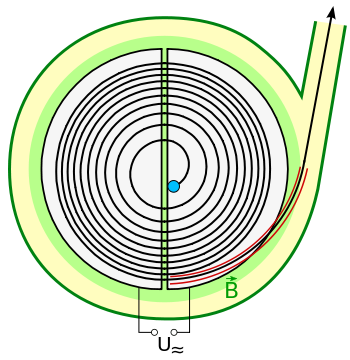
\includegraphics[width=0.35\textwidth]{Zyklotron_Prinzipskizze02.png}
%	\vspace{-13pt}
%	\caption{Prinzipskizze eines Zyklotrons}
%	\vspace{-5pt}	
%	
%\end{wrapfigure}

%\subsubsection{Anwendung}

% Some Formula:

%\begin{equation}
%	x= \frac{y \cdot 13 \pi z}
%			{\cos \alpha}
%\end{equation}


%%%%%%%%%%%%%%%%%%%%%%%%%%%
%%% Eigentlicher Beginn %%%
%%%%%%%%%%%%%%%%%%%%%%%%%%%

\subsection{Definitionen zu Schwingungen} \label{subsec:definitionenzuschwingungen}

Eine Schwingung bezeichnet eine periodische Energieumwandlung von einer in eine anderer Form von Energie und umgekehrt. \referenz{subsec:kenngroessen_schwingungen}


\subsubsection{Harmonische Schwingung}

Der zeitliche Verlauf einer harmonische Schwingung kann mit einer Sinuswelle beschrieben werden. Das mathematische Kriterium ist die Proportionalität der Rückstellkraft $F_{r}$ zum Betrag der Auslenkung $l$:

\begin{equation} \label{eq:kriterium_harmonisch}
	F_{r} \sim l
\end{equation}


\subsubsection{Schwingung}

Bei einer gedämpften Schwingung nimmt die Elongation über der Zeit ab. Außerhalb des im Physikunterricht angenommenen Modells sind alle Schwingung gedämpft, da Energie auch an die Umgebung abgegeben wird, beispielsweise durch Reibung in thermische Energie.



\subsection{Definitionen zu Wellen}

Als Welle bezeichnet man einen Vorgang bei dem Energie aber keine Masse transportiert wird. Es handelt sich um ein System gekoppelter Oszillatoren bei dem die Energie, die bei der Anregung eines Oszillators aufgewendet wird, vom diesem an die anderen Oszillatoren abgegeben wird. Daher wird die Energie räumlich transportiert, obwohl, absolut gesehen, sich jeder Oszillator noch stets an seinem Platz befindet.

\subsubsection{Transversalwelle}

Eine Transversalwelle ist eine Welle, deren Auslenkungsvektoren (= Richtung der Auslenkung) senkrecht auf der Ausbreitungsrichtung stehen.

Bsp.: Seilwelle, elektromagnetische Wellen (bei $ 400nm \leq \lambda \leq 700nm $: Licht)

\subsubsection{Longitudinalwelle}

Eine Longitudinal ist eine Welle, deren Auslenkungsvektoren (= Richtung der Auslenkung) parallel auf der Ausbreitungsrichtung stehen.

Bsp.: Schallwellen

















\section{Schwingungen} \label{sec:schwingungen}
%%%%% Kompendium -- Wellen und Optik %%%%%
%% Schwingungen %%


%Some sample text to be displayed above the first subsection

%\subsection{Prinzip}

%Ein Zyklotron besteht aus Zwei hohlen, halbzylindrischen und Duanden an denen eine Spannung mit unterschiedlichem Vorzeichen anliegt, und darüber bzw. darunter liegende Magneten, die ein homogenes Magnetfeld erzeugen. Zudem gibt es einen Einlass und einen Auslass für Teilchen.

%\begin{wrapfigure}{r}{0.4\textwidth} \label{Zyklo}
%
%	\vspace{-10pt}
%	\includegraphics[width=0.35\textwidth]{Zyklotron_Prinzipskizze02.png}
%	\vspace{-13pt}
%	\caption{Prinzipskizze eines Zyklotrons}
%	\vspace{-5pt}	
%	
%\end{wrapfigure}

%\subsubsection{Anwendung}

% Some Formula:

%\begin{equation}
%	x= \frac{y \cdot 13 \pi z}
%			{\cos \alpha}
%\end{equation}

%%%%%%%%%%%%%%%%%%%%%%%
% Eigentlicher Beginn %
%%%%%%%%%%%%%%%%%%%%%%%


\subsection{Diagramm einer Schwingung} \label{subsec:diagramm_schwingung}

\begin{figure}[h!]


	\includegraphics[width=0.9\textwidth]{Pictures/schwingung}

	\caption{Diagramm einer Schwingung: Elongation über der Zeit}

	
\end{figure}

\subsection{Kenngrößen von Schwingungen} \label{subsec:kenngroessen_schwingungen}


\subsubsection[Amplitude]{Amplitude: $y_{max}$ o. $s_{max}$ o. $\hat{y}$ o. $\hat{s}$ (Basiseinheit: $m$)}

Die maximale Elongation (=\glqq Auslenkung\grqq) der Schwingung.


\subsubsection[Periodendauer]{Periodendauer: $T$ (Basiseinheit: $s$)}
	
Die Zeit, die es dauert bis der schwindende Körper an der selben Stelle von der selben Richtung aus angelangt ist. Beispielsweise vom positiven Schwingungsmaximum (\glqq Berg\grqq) zum nächsten oder von der Nullstelle (\glqq Ruhelage\grqq) zur 2. darauffolgenden Nullstelle.

Davon abgeleitet:
\begin{itemize}
	\item Frequenz: $f=\frac{1}{T}$ (Basiseinheit: $Hz=\frac{1}{s}$)
	
	Anzahl der Perioden pro Sekunde.
	\item Winkelgeschwindigkeit: $\omega=2 \pi f=\frac{2 \pi}{T}$ (Basiseinheit: $\frac{rad}{s}$)
		
	Änderung des Winkels über der Zeit, wobei eine ganze Periode mit $360 \degree$ im Grad oder, im Physikunterricht verwendet, mit $2 \pi$ im Bogenmaß (eng: \glqq Radian\grqq) bezeichnet wird.\footnote{Umrechnung des Winkels $\alpha$ von Grad nach Bogenmaß: $\alpha_{rad} = \alpha_{deg} \cdot \frac{2\pi}{360 \degree} = \alpha_{deg} \cdot \frac{\pi}{180 \degree} $}
\end{itemize}


\subsubsection[Phasenverschiebung]{Phasenverschiebung: $\phi$ (Basiseinheit: $rad$)}
	
Wenn sich der Schwingungskörper zum Startzeitpunkt $t=0$ nicht in der Ruhelage $y=0$ befindet muss die Phasenverschiebung, z.B. zur Aufstellung der Schwingungsgleichung (\referenz{subsec:schwingungsgleichungen}), berücksichtigt werden. Die Phasenverschiebung gibt den Abstand von der y-Achse zum nächsten Durchlauf der Ruhelage von der negativen Seite.

	\begin{wrapfigure}{r}{0.5\textwidth} \label{phasenverschiebung}
	
		\vspace{-10pt}
		\includegraphics[width=0.48\textwidth]{Pictures/phasenverschiebung}
		\vspace{-13pt}
		\caption{Phasenverschiebung um $+\frac{3\pi}{2}$}
		\vspace{-5pt}
	
	\end{wrapfigure}

Im nebenstehenden Diagramm beträgt die Phasenverschiebung $\phi = +\frac{3\pi}{2}$, also ein Drei-Viertel der Periode. Man könnte ebenfalls sagen, die Phasenverschiebung beträgt $\phi = -\frac{\pi}{2}$, also minus Ein-Viertel der Periode. Beides ist äquivalent, jedoch ist es leichter mit einer positiven Phasenverschiebung zu rechnen.
	
	


\subsection{Schwingungsgleichungen} \label{subsec:schwingungsgleichungen}

Daraus ergibt sich folgende Schwingungsgleichung, bzw. Schwingungsfunktion, für eine harmonische Schwingung (\referenz{sec:definitionen}), die die Elongation in Abhängigkeit der Zeit angibt:

\begin{equation} \label{eq:schwingungsgleichung_y}
	y(t)=y_{max} \cdot \sin{(\omega t + \phi)}
\end{equation}

Die erste Ableitung dieser Gleichung nach $t$ gibt die Geschwindigkeit des Schwing-körpers zur Zeit $t$ an:

\begin{equation} \label{eq:schwingungsgleichung_v}
	y'(t)=v(t)=y_{max} \cdot \omega \cdot \cos{(\omega t + \phi)}
\end{equation}

Die zweite Ableitung gibt die Beschleunigung des Schwingkörpers zur Zeit $t$ an:

\begin{equation} \label{eq:schwingungsgleichung_a}
	y''(t)=v'(t)=a(t)=y_{max} \cdot \omega^{2} \cdot -\sin{(\omega t + \phi)}
\end{equation}


\subsection{Weitere Gleichungen und Gesetze}

\subsubsection{Gesetze im Kreis}

\paragraph{Bahngeschwindigkeit im Kreis}

Die Bahngeschwindigkeit gibt in absoluten Einheiten ($\frac{m}{s}$) an, wie schnell sich das Objekt auf der Bahn fortbewegt. Zusätzlich zur Winkelgeschwindigkeit (\referenz{subsec:kenngroessen_schwingungen}) muss bei der Kreisbahn daher noch der Radius bekannt sein:

\begin{equation*} \label{eq:bahngeschwindigkeit}
	v=\frac{2r\pi}{T}=\omega r
\end{equation*}

Eine andere Herleitung aus dem Kreisumfang $U=2r\pi$, der Periodendauer $T$ und der generellen Formel für Bahngeschwindigkeit $v=\frac{s(t)}{t}$ könnte wie folgt Aussehen:

\begin{align*}
	v&=\frac{s(t)}{t} \\
	v&=\frac{2r\pi}{T}
\end{align*}


\paragraph{Zentripetalbeschleunigung}

Um auf einer Kreisbahn zu bleiben, muss eine Zentripedalbeschleunigung auf einen Körper wirken, die zum Kreiszentrum hin zeigt. Die Formel lautet:

\begin{equation*}
	a_z=\frac{v^2}{r}=\omega^2 r
\end{equation*}


\paragraph{Zentripetalkraft}

Dies ist die Kraft, die auf einen Körper ausgewirkt werden muss, damit er auf einer Kreisbahn bleibt. Zusätzlich zur Zentripetalbeschleunigung muss nun also noch gemäß Newtons zweiten Axiom $F=a \cdot m$ die Masse als Faktor in die Gleichung aufgenommen werden:

\begin{align*}
	F_z &= a_z \cdot m \\
	F_z &= \frac{v^{2}m}{r}
\end{align*}


\subsubsection{Gesetze bei Geschwindigkeiten}

Aus der maximalen Geschwindigkeit und der Frequenz, Periodendauer oder Winkelgeschwindigkeit lässt sich sofort auf die Amplitude schließen, da in der Funktion für die Geschwindigkeit bei einer Schwingung (\referenz{subsec:schwingungsgleichungen}) $v(t)=\omega \cdot y_{max} \cdot \cos{(\omega t)}$ das Maxima dann erreicht ist, wenn der Cosinus seinen Maximalwert $1$ annimmt. Dann gilt folgendes:

\begin{align*} \label{eq:geschwindigkeit_amplitude}
	v_{max} &= \omega \cdot y_{max} \\
	v_{max} &= 2\pi f \cdot y_{max} \\
	y_{max} &= \frac{v_{max}}{2\pi f}
\end{align*}


\subsubsection{Gesetze am Federpendel}

\paragraph{Hooke'sches Gesetz}

Das Hooke'sche Gesetz gibt die Federhärte einer Feder, also dessen Kenngröße, an. Die Einheit $\frac{N}{m}$ erklärt selbst die Formel:

\begin{equation*}
	D=\frac{F}{l}
\end{equation*}

Mit dem Gesetz ist gezeigt, dass an einem Federpendel die Rückstellkraft $F$ proportional zur Auslenkung $l$ ist. Damit ist es eine harmonische Schwingung. (\referenz{subsec:definitionenzuschwingungen})

\paragraph{Periodendauer beim Federpendel}

Die Periodendauer beim Federpendel ist abhängig von der Masse $m$ und der Federkonstante $D$:

\begin{equation*}
	T_{Feder}=2\pi \cdot \frac{m}{D}
\end{equation*}

Die Herleitung gestaltet sich folgendermaßen: Die zur Auslenkung $y$ proportionale Kraft $F$ ist die Rückstellende Kraft; beschrieben durch eine Umformung des Hooke'schen Gesetzes: $F_{r}=D \cdot y$. 
%Der Vektor dieser Rückstellende Kraft zeigt dem der Auslenkenden Kraft genau entgegen, daher muss der Term in diesem Fall negiert werden: $F_{r}=-D \cdot y$.

In einem geschlossenen System ist die Summe aller Kräfte $0$. Es ergibt sich Folgendes:

\begin{align*}
	F_a + F_r &= 0 \\
	F_a &= -F_r \\
\end{align*}

Die Kraft $F_a$ kann wie jede Kraft mit Newtons zweitem Gesetz als $F_a=m \cdot a$ beschrieben werden. Die Beschleunigung in $a$ kann dann als zweite Ableitung der Auslenkung $y$ nach der Zeit beschrieben werden. Aus den Schwingungsgleichungen (\referenz{subsec:schwingungsgleichungen}) geht hervor, dass $y''=-\omega^{2} \cdot y$ ist. Daher kann man wie folgt einsetzen:

\begin{align*}
	m \cdot a &= -D \cdot y \\
	m \cdot y'' &= -D \cdot y \\
	m \cdot -\omega^{2} \cdot y &= -D \cdot y \\
	- m \cdot \omega^{2} &= -D \\
	\omega &= \sqrt{\frac{D}{m}}
\end{align*}

Für aus $\omega=\frac{2\pi}{T}$ folgt für $T$:

\begin{equation*}
	T = 2\pi \cdot \sqrt{\frac{m}{D}}
\end{equation*}














\section{Wellen -- Mathematisierung} \label{sec:wellen}
%%%%% Physik Kompendikum -- Wellen und Optik %%%%%
%% 03 Wellen %%


%Some sample text to be displayed above the first subsection

%\subsection{Prinzip}

%Ein Zyklotron besteht aus Zwei hohlen, halbzylindrischen und Duanden an denen eine Spannung mit unterschiedlichem Vorzeichen anliegt, und darüber bzw. darunter liegende Magneten, die ein homogenes Magnetfeld erzeugen. Zudem gibt es einen Einlass und einen Auslass für Teilchen.

%\begin{wrapfigure}{r}{0.4\textwidth} \label{Zyklo}
%
%	\vspace{-10pt}
%	\includegraphics[width=0.35\textwidth]{Zyklotron_Prinzipskizze02.png}
%	\vspace{-13pt}
%	\caption{Prinzipskizze eines Zyklotrons}
%	\vspace{-5pt}	
%	
%\end{wrapfigure}

%\subsubsection{Anwendung}

% Some Formula:

%\begin{equation}
%	x= \frac{y \cdot 13 \pi z}
%			{\cos \alpha}
%\end{equation}

%%%%%%%%%%%%%%%%%%%%%%%
% Eigentlicher Beginn %
%%%%%%%%%%%%%%%%%%%%%%%

\subsection{Diagramme von Wellen} \label{subsec:diagramm_welle}

Einer Welle reicht ein Diagramm zur Darstellung nicht aus. Da es sehr viele Oszillatoren gibt, die alle zu unterschiedlichen Zeiten zu schwingen beginnen, bräuchte man ein Elongation-Zeit-Diagramm (\referenz{subsec:diagramm_schwingung}) für jedes Teilchen, oder ein 3-dimensionales Diagramm.

Allerdings reichen zwei Diagramme, davon ein Elongation-Zeit-Diagramm eines beliebigen Teilchens und ein Elongation-Strecke-Diagramm (auch bekannt als \glqq Standbild\grqq) zu einem beliebigen Zeitpunkt, um alle Kenngrößen der Welle erfassen zu können.



\subsection{Kenngrößen}


\subsubsection[Amplitude]{Amplitude: $y_{max}$ o. $s_{max}$ o. $\hat{y}$ o. $\hat{s}$ (Basiseinheit: $m$)}

\textbf{Kategorie: Schwingung \textit{eines} Oszillators}

Die maximale Elongation (=\glqq Auslenkung\grqq) der Schwingungen der einzelnen Oszillatoren.



\subsubsection[Periodendauer]{Periodendauer: $T$ (Basiseinheit: $s$)}

\textbf{Kategorie: Schwingung \textit{eines} Oszillators}
	
Die Zeit, die es dauert bis einer der schwindenden Körper an der selben Stelle von der selben Richtung aus angelangt ist. Beispielsweise vom positiven Schwingungsmaximum (\glqq Berg\grqq) zum nächsten oder von der Nullstelle (\glqq Ruhelage\grqq) zur 2. darauffolgenden Nullstelle.

Davon abgeleitet:
\begin{itemize}
	\item Frequenz: $f=\frac{1}{T}$ (Basiseinheit: $Hz=\frac{1}{s}$)
	
	Anzahl der Perioden pro Sekunde.
	\item Winkelgeschwindigkeit: $\omega=2 \pi f=\frac{2 \pi}{T}$ (Basiseinheit: $\frac{rad}{s}$)
		
	Änderung des Winkels über der Zeit, wobei eine ganze Periode mit $360 \degree$ im Grad oder, im Physikunterricht verwendet, mit $2 \pi$ im Bogenmaß (eng: \glqq Radian\grqq) bezeichnet wird.\footnote{Umrechnung des Winkels $\alpha$ von Grad nach Bogenmaß: $\alpha_{rad} = \alpha_{deg} \cdot \frac{2\pi}{360 \degree} = \alpha_{deg} \cdot \frac{\pi}{180 \degree} $}
\end{itemize}



\subsubsection[Wellenlänge]{Wellenlänge: $\lambda$ (Basiseinheit: $m$)}

\textbf{Kategorie: Oszillatorsystem}

Der räumliche Abstand zwischen 2 Wellenbergen im Elongation-Strecke-Diagramm, der Abstand eines Nulldurchlaufs mit dem zweiten darauffolgenden.



\subsubsection[Ausbreitungsgeschwindigkeit]{Ausbreitungsgeschwindigkeit: $c$ (Basiseinheit: $\frac{m}{s}$)}

Die Ausbreitungsgeschwindigkeit ist eigentlich keine echte Kenngröße, da sie nicht in der Wellengleichung auftaucht. Trotzdem ist sie hilfreich um $\lambda$ oder $f$ zu berechnen. Die Gleichung lautet:

\begin{equation} \label{eq:wellen_c}
	c=\lambda \cdot f=\frac{\lambda}{T}
\end{equation}



\subsection{Wellengleichungen}

Die Wellengleichung gibt die Elongation des Teilchens mit dem Abstand $x$ zum Ausgangspunkt zum Zeitpunkt $t$ an:

\begin{equation} \label{eq:wellengleichung_y}
	y(x,t) = y_{max} \cdot sin{ (2\pi(\frac{t}{T}-\frac{x}{\lambda})) }
\end{equation}

Zur Herleitung aus der Schwingungsgleichung muss Folgendes beachtet werden. Die Zeit $t_x$ bis das räumliche Teilchen $x$ von der Front der Welle erfasst wird, lässt sich recht einfach berechnen. Gebraucht wird dabei die Ausbreitungsgeschwindigkeit $c=\frac{\lambda}{T}$ die generelle Formulierung der Geschwindigkeit $v=\frac{s}{t}$:

\begin{align*}
	t   &= \frac{s}{v} \\
	t_x &= \frac{x}{c} \\
	t_x &= \frac{x \cdot T}{\lambda}
\end{align*}

Analog zur Verschiebung nach rechts von beispielsweise einer Parabel, muss der Term für $t_x$ von $t$ in der Schwingungsgleichung abgezogen werden. Damit ist die Variable $x$ mit in der Gleichung und der Term \glqq kompensiert\grqq{} den \glqq Offset\grqq{}, der sich durch das spätere Erfassen ergibt:

\begin{align*}
	y(x,t) &= y_{max} \cdot sin{[\omega \cdot (t-\frac{x}{\lambda} \cdot T)]} \\
	y(x,t) &= y_{max} \cdot sin{[\frac{2\pi}{T} \cdot (t-\frac{x}{\lambda} \cdot T)]} \\
	y(x,t) &= y_{max} \cdot sin{[2\pi \cdot (\frac{t}{T}-\frac{x}{\lambda \cdot T} \cdot T)]} \\
	y(x,t) &= y_{max} \cdot sin{[2\pi \cdot (\frac{t}{T}-\frac{x}{\lambda})]}
\end{align*}



\subsection{Weitere Gleichungen und Gesetze}

\subsubsection{Wellenfront}

\paragraph{Erreichen eines beliebigen Teilchens}

Analog zu $v=\frac{s}{t}$:

\begin{equation*}
	t=\frac{x}{\lambda}
\end{equation*}















\section{Wellen -- Eigenschaften und Phänomene} \label{sec:wellen_eigenschaften}
%%%%% Kompendium -- Wellen und Optik %%%%%
%% Wellen -- Eigenschaften und Phänomene %%


%Some sample text to be displayed above the first subsection

%\subsection{Prinzip}

%Ein Zyklotron besteht aus Zwei hohlen, halbzylindrischen und Duanden an denen eine Spannung mit unterschiedlichem Vorzeichen anliegt, und darüber bzw. darunter liegende Magneten, die ein homogenes Magnetfeld erzeugen. Zudem gibt es einen Einlass und einen Auslass für Teilchen.

%\begin{wrapfigure}{r}{0.4\textwidth} \label{Zyklo}
%
%	\vspace{-10pt}
%	\includegraphics[width=0.35\textwidth]{Zyklotron_Prinzipskizze02.png}
%	\vspace{-13pt}
%	\caption{Prinzipskizze eines Zyklotrons}
%	\vspace{-5pt}	
%	
%\end{wrapfigure}

%\subsubsection{Anwendung}

% Some Formula:

%\begin{equation}
%	x= \frac{y \cdot 13 \pi z}
%			{\cos \alpha}
%\end{equation}

%%%%%%%%%%%%%%%%%%%%%%%
% Eigentlicher Beginn %
%%%%%%%%%%%%%%%%%%%%%%%

Im Folgenden werden bei der Nennung von \glqq Wellen\grqq{} immer Transversalwellen gemeint, wenn es keine weitere Anmerkung gibt.  



\subsection{Reflexion}  

	\paragraph{Fixiertes Ende}
	
	Wenn eine Welle von einem fixierten Ende (eingespannt) reflektiert wird, dann gibt es einen Phasensprung von $180 \degree$ oder $\pi$, bzw $\frac{T}{2}$.
	
	\paragraph{Loses Ende}
	
	Trifft eine Welle auf ein loses Ende, dann wird sie ohne  Phasensprung reflektiert.



\subsection{Überlagerung}

Wenn sich Wellen in einem räumlichen Punkt treffen, dann überlagern sie sich und bilden eine summierte Welle. Wenn also ein Wellenberg auf einen Wellenberg trifft, addieren sich beide Welle und der resultierende Wellenberg ist höher. Sollte auf einen Wellenberg ein Wellental treffen wird auf addiert, und die resultierende Welle von der Amplitude her kleiner.

Nachdem sich die Wellen in diesem Punkt überlagert haben, laufen beide weiter ohne die andere zu beeinflussen; so als hätte es die Überlagerung nie gegeben.

	\subsubsection{Stehende Welle}
	
	Wenn sich gegenläufige, das heißt parallel und identisch, aber in die entgegengesetzte Richtung fortschreitende, Wellen mit derselben Wellenlänge überlagern, entsteht eine stehende Welle. 
	Das heißt, dass es mindestens 2 Oszillatoren auf dieser Welle gibt, die sich gar nicht bewegen (\glqq stehen\grqq), die sogenannten Knotenpunkte.
	
	Eine stehende Welle kann zum Beispiel ausgelöst werden, wenn bei einer Reflexion am festen Ende die Hälfte der Wellenlänge $\lambda$ ein ganzzahliges Vielfaches der Abstands $l$ der beiden Enden ist. $k$ ist in diesem Fall eine Variable, die nur positive ganze Zahlen annehmen kann:
	
	\begin{equation} \label{stehendewelle}
		\lambda = 2k \cdot l \ \ \ wobei \ \ k \in 1,2,3...
	\end{equation}



\subsection{Interferenzen} \label{sec:interferenz}

Wenn sich Wellen, die nicht nur dieselbe Wellenlänge, sondern auch die selbe Amplitude aufweisen, in einem Punkt überlagern, dann kann es zu Interferenzen kommen.

	\subsubsection{Konstruktive Interferenz}
	
	Wenn in dem Punkt beide Wellen ein Maximum aufweisen, sich also zu einem höheren Wellenberg addieren, spricht man von konstruktiver Interferenz.
	
	Dazu muss der Gangunterschied $\delta$ ein ganzzahliges Vielfaches der Wellenlänge sein:
	
	\begin{equation}	\label{eq:kon_interferenz}
		\delta = k \cdot \lambda \ \ \ wobei \ \ k \in 1,2,3...
	\end{equation}
	
	\subsubsection{Destruktive Interferenz}
	
	Im Gegensatz zur konstruktiven Interferenz, treffen nun also Wellen aufeinander, die einmal einen Wellenberg und einmal ein Wellental aufweisen. Da sie dieselbe Amplitude haben, ist die resultierende Amplitude im betroffenen Punkt $0$.
	
	Der Gangunterschied $\delta$ muss daher die Summe eines ganzzahliges Vielfaches Wellenlänge und der halben Wellenlänge sein:
	
	\begin{equation}
		\delta = k \cdot \lambda + \frac{\lambda}{2} \ \ \ wobei \ \ k \in 1,2,3...
	\end{equation}

	Zur einfacheren Umstellung nach $\lambda$ existiert diese, internationale Form:
	
	\begin{equation} \label{eq:des_interferenz}
		\delta = (2k -1) \cdot \frac{\lambda}{2} \ \ \ wobei \ \ k \in 1,2,3...
	\end{equation}



\subsection[Ausbreitung in Elementarwellen]{Ausbreitung in Elementarwellen (Huygens'sches Prinzip)} \label{subsec:ausbreitung}

Das Huygens'sche Prinzip macht eine wichtige Aussage zur Ausbreitung von Wellen:

\glqq Jedes Teilchen (Oszillator), das von einer Wellenfront erfasst wird, löst von sich aus eine zirkulare Welle nach allen Seiten aus.\grqq{} Die eigentlich sichtbare Wellenfront ist nach Huygens eine Einhüllende aller \glqq Elementarwellen\grqq . Dadurch ist es Wellen unter anderem möglich in den geometrischen Schattenraum zu propagieren. \referenz{subsec:doppelspalt}


\subsection{Wellen am Doppelspalt} \label{subsec:doppelspalt}

Wenn nun eine räumlich und zeitlich kohärente Wellen, das heißt Wellenfronten deren Wellen sowohl parallel als auch phasengleich (mit derselben Wellenlänge und Gangunterschied $\delta= k \cdot \lambda$) verlaufen, auf ein Hindernis mit 2 schmalen Spalten trifft, bildet sich folgendes Interferenzmuster:

%\begin{figure}[h!]
%	\center
%	\includegraphics[width=0.4\textwidth]{doppelspalt_wasser}
%	\caption{Eine kohärente Welle am Doppelspalt}
%\end{figure}

Dies ist mit dem Huygens'schen Prinzip (\referenz{subsec:ausbreitung}) zu erklären: Angenommen, in jedem Spalt gäbe es nur ein schwingendes Teilchen. Dieses wird von der Wellenfront erfasst und ist selber Auslöser einer zirkularen Wellen. Da dieser Oszillator an dieser Stelle der einzige ist, gibt es keine gerade Wellenfront als Einhüllende, sondern einzig die Zirkularwelle des angeregten Oszillators.


\subsubsection{Mathematisierung}

	Der Versuch ist auch mit Laserlicht, also Monochromatisch (eine einzige Wellenlänge) und Kohärent, durchführbar. Das Licht wird durch einen schmalen Doppelspalt mit dem Spaltabstand $d \leq 2mm$ hinter dem sich im Abstand $a$ ein Schirm befindet. 
	
	Auf dem Schirm ist ein Interferenzmuster zu beobachten. In der Mitte ist ein heller Streifen, links und rechts davon, symmetrisch, sind weniger intensive Lichtpunkte. Diese Punkte werden Maxima genannt, da in diesen Punkten konstruktive Interferenz herrscht (\referenz{sec:interferenz}). An den Minimalstellen herrschen destruktive Interferenzen. Der Gangunterschied ergibt sich hier durch den Unterschiedlichen Abstand der Punkte auf dem Schirm zu dem beiden Schlitzen.
	
	Eine Zeichnung:
	
%	\begin{figure}[h!]
%		\center
%		\includegraphics[width=0.8\textwidth]{default}
%		\caption{Das Maxima 1. Ordnung am Doppelspalt}
%	\end{figure}
	
	Die Winkel $\alpha_a$ und $\alpha_d$ sind gleich und werden im Folgen schlicht als $\alpha$ bezeichnet. Für $\alpha$ ergeben sich aus den trigonomischen Winkelfunktionen im rechtwinkligen Dreieck 2 Gleichungen: $sin{\alpha}=\frac{\delta}{d}$ und $tan{\alpha}=\frac{d_k}{a}$. Da $a>>d_k$ ist $\alpha<10 \degree$ und die Kleinwinkelnäherung $sin{\alpha} \approx \tan{alpha}$ kann verwendet werden. Der Gangunterschied $\delta$ muss der Bedingung für konstruktive Interferenz $\delta = k \cdot \lambda$ genügen (Siehe Gleichung \ref{eq:kon_interferenz} auf Seite \pageref{eq:kon_interferenz}). Daraus Ergibt sich:
	
	\begin{align}
		\sin{\alpha} &= \tan{\alpha} \\
		\frac{\delta}{d} &= \frac{d_k}{a} \\
		\frac{k \cdot \lambda}{d} &= \frac{d_k}{a}  \ \ \ wobei \ \ k \in 1,2,3... \\
		\lambda &= \frac{d_{k} \cdot d}{a \cdot k}  \ \ \ wobei \ \ k \in 1,2,3...
	\end{align}
	
	Für $k$ muss die Ordnung des betrachteten Maxima eingesetzt werden.
		

\subsubsection{Ohne Kleinwinkelnäherung}

	Um präziser ablesen zu können, kann ein Gitter statt einem Doppelspalt verwendet werden. Das Gitter weist einen wesentlich geringeren Abstand zwischen den Schlitzen auf (z.B. $\frac{1}{600}mm$), sodass die Interferenzmaxima deutlich weiter auseinander liegen. Der Fakt, dass der Lichtdurchsatz durch das Hinzufügen von mehr Schlitzen zu einem Gitter erhöht wurde, ändert nichts an den mathematischen Grundlagen des Versuchs.
	
	Allerdings geht mit dem größeren Abstand der Punkte auf dem Schirm die Gültigkeit der Kleinwinkelnäherung verloren. Allerdings kann die Größe des Winkels $\alpha_a$ über $\arctan{\frac{d_k}{a}}$ berechnet werden und in die Gleichung $\sin{\alpha} = \frac{\delta}{d}$ eingesetzt werden:
	
	\begin{align}
		\frac{\delta}{d} &= \sin{\alpha} \\
		 \delta &= \sin{(\arctan{\frac{d_k}{a}})} \cdot d \\
		\lambda \cdot k &= \sin{(\arctan{\frac{d_k}{a}})} \cdot d \ \ \ wobei \ \ k \in 1,2,3... \\
		\lambda &= \frac{\sin{(\arctan{\frac{d_k}{a}})} \cdot d}{k} \ \ \ wobei \ \ k \in 1,2,3...
	\end{align}


\subsection{Lichtspektrum am Doppelspalt}

Wenn ein Lichtspektrum (z.B. weißes Licht von einer Glühbirne) auf einen Doppelspalt oder ein Gitter trifft, dann tritt dasselbe Phänomen wie bei monochromatischem Licht, mit dem Unterschied, dass die unterschiedlichen Wellenlängen im Spektrum ihren eigenen, von der Wellenlänge abhängigen, Abstand $d_k$ haben. Dadurch wird das Lichtspektrum von violett bis rot aufgefächert (Dispersion).













\section{Elektromagnetische Wellen} \label{sec:em_wellen}
%%%%% TITLE OF MAIN DOCUMENT %%%%%
%% NUMBER AND TITLE OF SECTION %%


%Some sample text to be displayed above the first subsection

%\subsection{Prinzip}

%Ein Zyklotron besteht aus Zwei hohlen, halbzylindrischen und Duanden an denen eine Spannung mit unterschiedlichem Vorzeichen anliegt, und darüber bzw. darunter liegende Magneten, die ein homogenes Magnetfeld erzeugen. Zudem gibt es einen Einlass und einen Auslass für Teilchen.

%\begin{wrapfigure}{r}{0.4\textwidth} \label{Zyklo}
%
%	\vspace{-10pt}
%	\includegraphics[width=0.35\textwidth]{Zyklotron_Prinzipskizze02.png}
%	\vspace{-13pt}
%	\caption{Prinzipskizze eines Zyklotrons}
%	\vspace{-5pt}	
%	
%\end{wrapfigure}

%\subsubsection{Anwendung}

% Some Formula:

%\begin{equation}
%	x= \frac{y \cdot 13 \pi z}
%			{\cos \alpha}
%\end{equation}

%%%%%%%%%%%%%%%%%%%%%%%
% Eigentlicher Beginn %
%%%%%%%%%%%%%%%%%%%%%%%

Als elektromagnetische Wellen bezeichnet man alle Wellen, bei denen gekoppelten elektrischen und magnetische Felder schwingen. Die Schwingungsverktoren der beiden Felder stehen jeweils senkrecht aufeinander und senkrecht auf dem Vektor der Ausbreitungsrichtung:\footnote{„Onde electromagnetique“ von SuperManu - Self, based on Image:Onde electromagnetique.png. Lizenziert unter CC BY-SA 3.0 über Wikimedia Commons - \url{https://commons.wikimedia.org/wiki/File:Onde_electromagnetique.svg}}

\begin{figure}[h!]
	\center
	\includegraphics[width=0.8\textwidth]{em_welle}
	\caption{Eine elektromagnetische Welle}
\end{figure}

Im Vakuum bzw. in der Luft bewegen sich alle elektromagnetischen Wellen mit Lichtgeschwindigkeit fort. (Taschenrechner: Konstante 28: $c_0=299.792.458 \frac{m}{s}$)

\subsection{Spektrum}
\hspace{-60pt}
\begin{tabular}[c]{|c|c|c|l|}
	\hline
	Name				&	$f$						& $\lambda$ 	& Kommentar\\
	\hline
	Längstwellen		&	$15-200Hz$				& $10^6-10^7m$ & Strom; Nur Nahfeld\\
	Radiowellen			&	$10^4-10^8Hz$			& $10^0-10^4m$ & \\
	Mikrowellen			&	$10^8-10^{11}Hz$		& $10^{-3}-10^{0}m$ & \\
	Infrarotes Licht	&	$>10^{12}Hz$			& $<10^{-4}m$ & \glqq Wäremestrahlung\grqq \\
	Sichtbares Licht	&	$\approx 10^{15}Hz$		& $400-800nm$ $\approx 10^{-6}m$ & sichtbar\\
	Röntgenstrahlung	&	$10^{16} - 10^{20}Hz$	& $10^{-12}-10^{-8}m$ & Erzeugung: schnelle $e^{-}$ auf Metall \\
	Gammastrahlung		&	$>10^{20}Hz$			& $<10^{-12}m$ & \\
	\hline
\end{tabular}













\section{Optik} \label{sec:optik}
%%%%% Kompendium -- Wellen und Optik %%%%%
%% Optik %%


%Some sample text to be displayed above the first subsection

%\subsection{Prinzip}

%Ein Zyklotron besteht aus Zwei hohlen, halbzylindrischen und Duanden an denen eine Spannung mit unterschiedlichem Vorzeichen anliegt, und darüber bzw. darunter liegende Magneten, die ein homogenes Magnetfeld erzeugen. Zudem gibt es einen Einlass und einen Auslass für Teilchen.

%\begin{wrapfigure}{r}{0.4\textwidth} \label{Zyklo}
%
%	\vspace{-10pt}
%	\includegraphics[width=0.35\textwidth]{Zyklotron_Prinzipskizze02.png}
%	\vspace{-13pt}
%	\caption{Prinzipskizze eines Zyklotrons}
%	\vspace{-5pt}	
%	
%\end{wrapfigure}

%\subsubsection{Anwendung}

% Some Formula:

%\begin{equation}
%	x= \frac{y \cdot 13 \pi z}
%			{\cos \alpha}
%\end{equation}

%%%%%%%%%%%%%%%%%%%%%%%
% Eigentlicher Beginn %
%%%%%%%%%%%%%%%%%%%%%%%


\subsection{Brechung von Licht}

Wenn Licht von einem Medium in ein anderes übergeht wird es gebrochen, das heißt, es seine Richtung ändert sich. Die Brechung ist hauptsächlich vom Quotienten der Lichtgeschwindigkeiten in den Materialien abhängig, jedoch spielt auch die Wellenlänge eine Rolle, da kurzwelliges Licht etwas stärker gebrochen wird als langwelliges.

Brechung ist an folgendem Diagramm recht einfach mit dem Huygens'schen Prinzip (\referenz{subsec:ausbreitung}) zu erklären: \footnote{„Refraction - Huygens-Fresnel principle“ von Arne Nordmann (norro) - Own illustration, based on Image:Wellen-Brechung.png and Image:Huygens\_brechung.png. Lizenziert unter CC BY-SA 3.0 über Wikimedia Commons - \url{https://commons.wikimedia.org/wiki/File:Refraction\_-\_Huygens-Fresnel\_principle.svg}}

\begin{figure}[h!]
	\center
	\includegraphics[width=0.5\textwidth]{brechung}
	\caption{Brechung mit dem Huygens'schen Prinzip}
\end{figure}

Die Abbildung zeigt den Übergang eines schmalen, monochromatischen (nur eine Farbe/Wellenlänge) Lichtbündels in ein Material mit einer niedrigeren Lichtgeschwindigkeit. Das Lichtbündel ist faktisch eine phasengleiche Welle, die Schräg auf der Übergangsfläche auftrifft. So löst ein Wellenberg auf der linken Seite früher Elementarwellen aus als auf der rechten Seite. Da die Elementarwellen im neuen Medium langsamer sind als im alten wird der Lichtstrahl zum Lot hin gebrochen.

\subsubsection{Mathematisierung}

	Man denke sich nun ein senkrechtes Lot an die Kante des Materialübergangs. Die Winkel $\alpha$ sein der Winkel des Stahls im ersten Medium zum Lot und $\beta$ der Winkel des Strahls im neuen Medium zum Lot hin. Dann gilt folgendes:
	
	\begin{equation}
		\frac{sin{(\alpha)}}{sin{(\beta)}} = \frac{c_1}{c_2}
	\end{equation}
	
	Unter Berücksichtung der verschieden Brechungen von verschiedenen Wellenlängen muss eine neue Größe eingeführt werden, die Brechzahl $n$. Folgendes ergibt sich:
	
	\begin{equation} \label{eq:brechungsgesetz}
		\frac{sin{(\alpha)}}{sin{(\beta)}} = \frac{n_2}{n_1}
	\end{equation}











\chapter{Wellen} \label{ch:Wellen}
\section{Definitionen} \label{sec:definition_wellen}
Als Welle bezeichnet man einen Vorgang, bei dem Energie, aber keine Masse transportiert wird. Es handelt sich um ein System gekoppelter Oszillatoren, also schwingungsfähige Körper, bei dem die Energie, die bei der Anregung der Schwingung \emph{eines} Oszillators aufgewendet wird, vom diesem an andere, angrenzende Oszillatoren abgegeben wird. Daher wird die Energie räumlich transportiert, obwohl, absolut gesehen, sich jeder Oszillator noch stets an seinem Platz befindet.

\subsection{Transversalwelle}

Eine Transversalwelle ist eine Welle, deren Auslenkungsvektoren (= Richtung der Auslenkung) senkrecht auf der Ausbreitungsrichtung stehen.

Bsp.: Seilwelle, elektromagnetische Wellen (bei $ 400nm \leq \lambda \leq 700nm $: Licht, Siehe: \ref{sec:em_wellen})

\subsection{Longitudinalwelle}

Eine Longitudinalwelle ist eine Welle, deren Auslenkungsvektoren (= Richtung der Auslenkung) parallel auf der Ausbreitungsrichtung stehen.

Bsp.: Schallwellen

\section{Diagramme von Wellen} \label{sec:diagramm_wellen}
Einer Welle reicht ein Diagramm zur Darstellung nicht aus. Da es sehr viele Oszillatoren gibt, die alle zu unterschiedlichen Zeiten zu schwingen beginnen, bräuchte man ein Elongation-Zeit-Diagramm (\referenz{sec:diagramm_schwingung}) für jedes Teilchen, oder ein 3-dimensionales Diagramm.

Allerdings reichen zwei Diagramme, davon ein Elongation-Zeit-Diagramm eines beliebigen Teilchens und ein Elongation-Strecke-Diagramm (auch bekannt als \glqq Standbild\grqq) zu einem beliebigen Zeitpunkt, um alle Kenngrößen der Welle erfassen zu können.

\section{Kenngrößen} \label{sec:kenngroessen_wellen}
\subsection[Amplitude]{Amplitude: $y_{max}$ o. $s_{max}$ o. $\hat{y}$ o. $\hat{s}$ (Basiseinheit: $m$)}

\textbf{Kategorie: Schwingung \textit{eines} Oszillators}

\noindent Die maximale Elongation (=\glqq Auslenkung\grqq) der Schwingungen der einzelnen Oszillatoren.



\subsection[Periodendauer]{Periodendauer: $T$ (Basiseinheit: $s$)}

\textbf{Kategorie: Schwingung \textit{eines} Oszillators}
	
\noindent Die Zeit, die es dauert, bis \emph{einer} der schwindenden Körper an der selben Stelle von der selben Richtung aus angelangt ist. Beispielsweise vom positiven Schwingungsmaximum (\glqq Berg\grqq) zum nächsten oder von der Nullstelle (\glqq Ruhelage\grqq) zur 2. darauffolgenden Nullstelle.

Davon abgeleitet:
\begin{itemize}
	\item Frequenz: $f=\frac{1}{T}$ (Basiseinheit: $Hz=\frac{1}{s}$)

	Anzahl der Perioden pro Sekunde.
	\item Winkelgeschwindigkeit: $\omega=2 \pi f=\frac{2 \pi}{T}$ (Basiseinheit: $\frac{rad}{s}$)

	Änderung des Winkels über der Zeit, wobei eine ganze Periode mit $360 \degree$ im Grad oder, im Physikunterricht verwendet, mit $2 \pi$ im Bogenmaß (eng: \glqq Radian\grqq) bezeichnet wird.\footnote{Umrechnung des Winkels $\alpha$ von Grad nach Bogenmaß: $\alpha_{rad} = \alpha_{deg} \cdot \frac{2\pi}{360 \degree} = \alpha_{deg} \cdot \frac{\pi}{180 \degree} $}
\end{itemize}



\subsection[Wellenlänge]{Wellenlänge: $\lambda$ (Basiseinheit: $m$)}

\textbf{Kategorie: Oszillatorsystem zu \emph{einem} Zeitpunkt}

\noindent Der räumliche Abstand zwischen 2 Wellenbergen im Elongation-Strecke-Diagramm, der Abstand eines Nulldurchlaufs mit dem zweiten darauffolgenden.



\subsection[Ausbreitungsgeschwindigkeit]{Ausbreitungsgeschwindigkeit: $c$ (Basiseinheit: $\frac{m}{s}$)}

\noindent Die Ausbreitungsgeschwindigkeit ist eigentlich keine echte Kenngröße, da sie nicht in der Wellengleichung auftaucht. Trotzdem ist sie hilfreich um $\lambda$ oder $f$ zu berechnen. Da eine Geschwindigkeit generell als Strecke pro Zeit ($v=\frac{s}{t}$) definiert ist, ist die Wellenlänge die Strecke, die die Wellenfront nach einer Periode ($T$) zurückgelegt hat.

\begin{equation} \label{eq:wellen_c}
	c=\frac{\lambda}{T}=\lambda \cdot f
\end{equation}

\begin{Aufgabe}
	Stelle alle Kenngrößen sowie die Ausbreitungsgeschwindigkeit der Beispielwelle in den Diagrammen \ref{fig:welle_bei_x} und  \ref{fig:welle_zu_t} heraus.
\end{Aufgabe}

\section{Wellengleichung} \label{sec:wellengleichung}
Die Wellengleichung gibt die Elongation des Teilchens mit dem Abstand $x$ zum Ausgangspunkt zum Zeitpunkt $t$ an:

\begin{equation} \label{eq:wellengleichung_y}
	y(x,t) = y_{max} \cdot sin{ (2\pi(\frac{t}{T}-\frac{x}{\lambda})) }
\end{equation}

Zur Herleitung aus der Schwingungsgleichung muss Folgendes beachtet werden. Die Zeit $t_x$ bis das räumliche Teilchen $x$ von der Front der Welle erfasst wird, lässt sich recht einfach berechnen. Gebraucht wird dabei die Ausbreitungsgeschwindigkeit $c=\frac{\lambda}{T}$ die generelle Formulierung der Geschwindigkeit $v=\frac{s}{t}$:

\begin{align*}
	t   &= \frac{s}{v} \\
	t_x &= \frac{x}{c} \\
	t_x &= \frac{x \cdot T}{\lambda}
\end{align*}

Analog zur Verschiebung nach rechts von beispielsweise einer Parabel, muss der Term für $t_x$ von $t$ in der Schwingungsgleichung abgezogen werden. Damit ist die Variable $x$ mit in der Gleichung und der Term \glqq kompensiert\grqq{} den \glqq Offset\grqq{}, der sich durch das spätere Erfassen ergibt:

\begin{align*}
	y(x,t) &= y_{max} \cdot sin{[\omega \cdot (t-\frac{x}{\lambda} \cdot T)]} \\
	y(x,t) &= y_{max} \cdot sin{[\frac{2\pi}{T} \cdot (t-\frac{x}{\lambda} \cdot T)]} \\
	y(x,t) &= y_{max} \cdot sin{[2\pi \cdot (\frac{t}{T}-\frac{x}{\lambda \cdot T} \cdot T)]} \\
	y(x,t) &= y_{max} \cdot sin{[2\pi \cdot (\frac{t}{T}-\frac{x}{\lambda})]}
\end{align*}

\section{Weitere Gleichungen und Gesetze} \label{sec:wellengleichung}
Die Wellengleichung gibt die Elongation des Teilchens mit dem Abstand $x$ zum Ausgangspunkt zum Zeitpunkt $t$ an:

\begin{equation} \label{eq:wellengleichung_y}
	y(x,t) = y_{max} \cdot sin{ (2\pi(\frac{t}{T}-\frac{x}{\lambda})) }
\end{equation}

Zur Herleitung aus der Schwingungsgleichung muss Folgendes beachtet werden. Die Zeit $t_x$ bis das räumliche Teilchen $x$ von der Front der Welle erfasst wird, lässt sich recht einfach berechnen. Gebraucht wird dabei die Ausbreitungsgeschwindigkeit $c=\frac{\lambda}{T}$ die generelle Formulierung der Geschwindigkeit $v=\frac{s}{t}$:

\begin{align*}
	t   &= \frac{s}{v} \\
	t_x &= \frac{x}{c} \\
	t_x &= \frac{x \cdot T}{\lambda}
\end{align*}

Analog zur Verschiebung nach rechts von beispielsweise einer Parabel, muss der Term für $t_x$ von $t$ in der Schwingungsgleichung abgezogen werden. Damit ist die Variable $x$ mit in der Gleichung und der Term \glqq kompensiert\grqq{} den \glqq Offset\grqq{}, der sich durch das spätere Erfassen ergibt:

\begin{align*}
	y(x,t) &= y_{max} \cdot sin{[\omega \cdot (t-\frac{x}{\lambda} \cdot T)]} \\
	y(x,t) &= y_{max} \cdot sin{[\frac{2\pi}{T} \cdot (t-\frac{x}{\lambda} \cdot T)]} \\
	y(x,t) &= y_{max} \cdot sin{[2\pi \cdot (\frac{t}{T}-\frac{x}{\lambda \cdot T} \cdot T)]} \\
	y(x,t) &= y_{max} \cdot sin{[2\pi \cdot (\frac{t}{T}-\frac{x}{\lambda})]}
\end{align*}

\section{Wellenphänomene} \label{sec:phaenomene_wellen}
Im Folgenden werden bei der Nennung von \glqq Wellen\grqq{} immer Transversalwellen gemeint, wenn es keine weitere Anmerkung gibt.  


\subsection[Ausbreitung in Elementarwellen]{Ausbreitung in Elementarwellen (Huygens'sches Prinzip)} \label{subsec:ausbreitung}

Das Huygens'sche Prinzip macht eine wichtige Aussage zur Ausbreitung von Wellen:

\glqq Jedes Teilchen (Oszillator), das von einer Wellenfront erfasst wird, löst von sich aus eine zirkulare Welle nach allen Seiten aus.\grqq{} Die eigentlich sichtbare Wellenfront ist nach Huygens eine Einhüllende aller \glqq Elementarwellen\grqq . Dadurch ist es Wellen unter anderem möglich, in den geometrischen Schattenraum zu propagieren (Siehe: \referenz{sec:interferenz_spalt}).


\subsection{Reflexion}  \label{subsec:Reflexion}

	\subsubsection{Fixiertes Ende}
	
	Wenn eine Welle von einem fixierten Ende (eingespannt) reflektiert wird, dann gibt es einen Phasensprung von $180 \degree$ oder $\pi$, bzw $\frac{\lambda}{2}$.
	
	\subsubsection{Loses Ende}
	
	Trifft eine Welle auf ein loses Ende, dann wird sie ohne Phasensprung reflektiert.



\subsection{Überlagerung} \label{subsec:ueberlagerung}

Wenn sich Wellen in einem räumlichen Punkt treffen, dann überlagern sie sich und bilden eine summierte Schwingung. Wenn also ein Wellenberg auf einen Wellenberg trifft, addieren sich beide Wellen und das Teilchen in welchem sich die Wellen überlagern wird höher ausgelenkt, als wenn nur eine Welle das Teilchen auslenkt.

Sollte auf einen Wellenberg ein Wellental treffen, wird ebenfalls addiert, wobei dann das Resultat eine kleinere Amplitude ist.

Nachdem sich die Wellen in diesem Punkt überlagert haben, laufen beide weiter ohne die andere zu beeinflussen, so als hätte es die Überlagerung nie gegeben.


\subsection{Interferenzen} \label{subsec:interferenz}

Wenn sich Wellen, die eine identische Wellenlänge besitzen, in einem Punkt überlagern, dann kommt es zu zeitlich stabilen Interferenzen, weil nun die beiden Wellen aus den unterschiedlichen Richtungen mit der selben Frequenz Wellenberge und Wellentäler \glqq nachliefern\grqq{} und damit die Interferenz aufrecht erhalten bleibt.

Der Gangunterschied der beiden Wellen ist $\delta$: die Differenz der Strecken vom jeweiligen Ursprungspunkt (zwei Punkte, in denen die Wellen nicht phasenverschoben sind, also zum selben Zeitpunkt Maxima oder Minima, etc. auftreten) zu dem in Frage stehenden Überlagerungspunkt. Siehe Abbildung \ref{fig:gangunterschied}\endnote{\glqq Interferenzbedingungen\grqq{} von Till Blaha - Eigenes Werk. Lizenziert unter Gemeinfrei.}.

Für die beiden extremen Arten der Interferenz (konstruktiv und destruktiv) muss für $\delta$ eine bestimmte Interferenzbedingungen erfüllt sein.
 
\begin{figure}[!h]
		\centering
		\includegraphics[width=0.9\textwidth]{Interferenz}
		\begin{comment} gnuplot './plot_noticszero.p'
set output 'plot_inteferenzhelper.png'
plot sin(x) ls 3
		\end{comment}
		\caption{$P_1$ und $P_2$ sind die Ursprungspunkte in denen Phasengleichheit herrscht. Die Differenz der Strecken $s_1$ und $s_2$ ist der Gangunterschied $\delta$. Die beiden Elongation-Zeit-Diagramme sollen die zeitliche Phasengleichheit in den beiden Ausgangspunkten zeigen.}
		\label{fig:gangunterschied}
\end{figure}

	\subsubsection{Konstruktive Interferenz}
	
	Bei der konstruktiven Interferenz ist die resultierende Amplitude genau die Addition der Amplituden der Ausgangswellen; das doppelte einer Amplitude, wenn beide Ausgangswellen identische Amplituden besitzen.
	
	Dazu müssen die Wellen im Interferenzpunkt zur selben Zeit Maxima und Minima aufweisen, also muss der Gangunterschied ein ganzzahliges Vielfaches der Wellenlänge sein:
	
	\begin{align}	\label{eq:kon_interferenz}
	\begin{split}
		\delta = k \cdot \lambda \quad \text{wobei} \ k \in 0,1,2...
	\end{split}
	\end{align}
	
	\subsubsection{Destruktive Interferenz}
	
	Bei der destruktiven Interferenz ist die resultierende Amplitude 0, wenn man davon ausgeht, dass die einfallenden Wellen die gleiche Amplitude haben
	
	Der Gangunterschied $\delta$ muss daher die Summe eines ganzzahliges Vielfaches Wellenlänge und der halben Wellenlänge sein, sodass sich immer ein Schwingungsberg und Schwingungstal überlagern und auslöschen.
	
	\begin{align}	\label{eq:des_interferenz}
	\begin{split}
		\delta &= k \cdot \lambda - \frac{\lambda}{2} \quad \text{wobei} \ k \in 1,2,3... \\
		\delta &= \lambda \cdot (k - \frac{1}{2}) \quad \text{wobei} \ k \in 1,2,3... 
	\end{split}
	\end{align}
	

\subsection{Stehende Welle}
	
Wenn sich gegenläufige Wellen, das heißt parallel und identisch, aber sich in die entgegengesetzte Richtung ausbreitende Wellen, mit derselben Wellenlänge überlagern, entsteht eine stehende Welle. 

Das heißt, dass es mindestens 2 Punkte auf gibt, in denen sich die Oszillatoren gar nicht bewegen (\glqq stehen\grqq), die sogenannten Knotenpunkte, in welchen destruktive Interferenz herrscht. Gleichzeitig gibt es auch immer mindestens einen Punkt, in welchem konstruktive Interferenz herrscht.
	
Eine stehende Welle kann zum Beispiel ausgelöst werden, wenn bei einer Reflexion am festen Ende die Hälfte der Wellenlänge $\lambda$ ein ganzzahliges Vielfaches der Abstands $l$ der beiden Enden ist. $k$ ist in diesem Fall eine Variable, die nur positive ganze Zahlen annehmen kann:
	
	\begin{align} \label{eq:stehendewelle}
		l = \frac{k \cdot \lambda}{2} \quad wobei \ k \in 1,2,3...
	\end{align}
	
	
\subsubsection{Beispiel}

Wer Gitarre spielt, erlebt, idealisiert, eine stehende Welle mit $k=0$, wenn er eine offene Saite anschlägt. (Abbildung \ref{fig:grundton})

\begin{figure}[!h]
		\centering
		\includegraphics[width=0.9\textwidth]{0Ordnung}
		\caption{Der Grundton auf der zweiten Saite von unten: $A2 \widehat{=} 110Hz$}
		\label{fig:grundton}
\end{figure}

Legt man nun beim Anschlagt einen Finger auf die Saite bei der Hälfte der Länge ohne die Saite herunter zu drücken, erhält man eine stehende Welle mit $k=1$; über dem 12. Bund, wo der Finger die Saite dämpft ist der 3. Knotenpunkt und es gibt 2 Stellen mit konstruktiver Interferenz. (Abbildung \ref{fig:ersteroberton})


Sollte man die Saite \glqq dritteln\grqq , also den Finger über dem 7. Bund (oder 24. Bund) auf die Saite legen, erhält man eine stehende Welle mit $k=2$; es gibt nun insgesamt 4 Knotenpunkte (an Sattel und Brücke, also da, wo die Saite eingespannt ist, unter dem Finger am 7. Bund und am leeren 24. Bund) und 3 konstruktive Interferenzen (Zwischen dem Satten und dem 7. Bund; zwischen dem 7. und 24. Bund; zwischen dem 24. Bund und der Brücke).(Abbildung \ref{fig:zweiteroberton}\endnote{\glqq Stehende Wellen bei Flageoletttönen bei Gitarren\grqq{} von Till Blaha - Eigenes Werk. Lizenziert unter Gemeinfrei.})

\begin{Aufgabe}
Die Mensur einer Gitarre ist an jeder Saite annähernd gleich. Warum ergeben sich trotzdem die unterschiedliche Tonhöhen (Frequenzen) an den einzelnen Saiten, wenn man sie offen spielt (nur anzupft, ohne etwas zu greifen)?

Hinweis 1: Die Mensur, also die Länge der Saite, ist in diesem Fall die Wellenlänge.

Hinweis 2: \gleichungsreferenz{eq:wellen_c}
\end{Aufgabe}

\begin{figure}[!h]
		\centering
		\includegraphics[width=0.8\textwidth]{1Ordnung_Final}
		\caption{Der 1. Oberton auf der zweiten Saite von unten: $A3 \widehat{=} 220Hz$; eine Oktave über dem Grundton}
		\label{fig:ersteroberton}
\end{figure}

\begin{figure}[!h]
		\centering
		\includegraphics[width=0.8\textwidth]{2Ordnung_Final}
		\caption{Der 2. Oberton auf der zweiten Saite von unten: $E4 \widehat{=} 330Hz$; eine Oktave und eine Quinte über dem Grundton}
		\label{fig:zweiteroberton}
\end{figure}





\chapter{Optik} \label{ch:Optik}
\section{Elektromagnetische Wellen} \label{sec:em_wellen}
%%%%% TITLE OF MAIN DOCUMENT %%%%%
%% NUMBER AND TITLE OF SECTION %%


%Some sample text to be displayed above the first subsection

%\subsection{Prinzip}

%Ein Zyklotron besteht aus Zwei hohlen, halbzylindrischen und Duanden an denen eine Spannung mit unterschiedlichem Vorzeichen anliegt, und darüber bzw. darunter liegende Magneten, die ein homogenes Magnetfeld erzeugen. Zudem gibt es einen Einlass und einen Auslass für Teilchen.

%\begin{wrapfigure}{r}{0.4\textwidth} \label{Zyklo}
%
%	\vspace{-10pt}
%	\includegraphics[width=0.35\textwidth]{Zyklotron_Prinzipskizze02.png}
%	\vspace{-13pt}
%	\caption{Prinzipskizze eines Zyklotrons}
%	\vspace{-5pt}	
%	
%\end{wrapfigure}

%\subsubsection{Anwendung}

% Some Formula:

%\begin{equation}
%	x= \frac{y \cdot 13 \pi z}
%			{\cos \alpha}
%\end{equation}

%%%%%%%%%%%%%%%%%%%%%%%
% Eigentlicher Beginn %
%%%%%%%%%%%%%%%%%%%%%%%

Als elektromagnetische Wellen bezeichnet man alle Wellen, bei denen gekoppelten elektrischen und magnetische Felder schwingen. Die Schwingungsverktoren der beiden Felder stehen jeweils senkrecht aufeinander und senkrecht auf dem Vektor der Ausbreitungsrichtung:\footnote{„Onde electromagnetique“ von SuperManu - Self, based on Image:Onde electromagnetique.png. Lizenziert unter CC BY-SA 3.0 über Wikimedia Commons - \url{https://commons.wikimedia.org/wiki/File:Onde_electromagnetique.svg}}

\begin{figure}[h!]
	\center
	\includegraphics[width=0.8\textwidth]{em_welle}
	\caption{Eine elektromagnetische Welle}
\end{figure}

Im Vakuum bzw. in der Luft bewegen sich alle elektromagnetischen Wellen mit Lichtgeschwindigkeit fort. (Taschenrechner: Konstante 28: $c_0=299.792.458 \frac{m}{s}$)

\subsection{Spektrum}
\hspace{-60pt}
\begin{tabular}[c]{|c|c|c|l|}
	\hline
	Name				&	$f$						& $\lambda$ 	& Kommentar\\
	\hline
	Längstwellen		&	$15-200Hz$				& $10^6-10^7m$ & Strom; Nur Nahfeld\\
	Radiowellen			&	$10^4-10^8Hz$			& $10^0-10^4m$ & \\
	Mikrowellen			&	$10^8-10^{11}Hz$		& $10^{-3}-10^{0}m$ & \\
	Infrarotes Licht	&	$>10^{12}Hz$			& $<10^{-4}m$ & \glqq Wäremestrahlung\grqq \\
	Sichtbares Licht	&	$\approx 10^{15}Hz$		& $400-800nm$ $\approx 10^{-6}m$ & sichtbar\\
	Röntgenstrahlung	&	$10^{16} - 10^{20}Hz$	& $10^{-12}-10^{-8}m$ & Erzeugung: schnelle $e^{-}$ auf Metall \\
	Gammastrahlung		&	$>10^{20}Hz$			& $<10^{-12}m$ & \\
	\hline
\end{tabular}












\section{Brechung} \label{sec:brechung}
Wenn Licht von einem Medium in ein anderes übergeht, wird es gebrochen, das heißt, es ändert seine Ausbreitungsrichtung. Die Brechung ist hauptsächlich vom Quotienten der Lichtgeschwindigkeiten in den beiden Materialien abhängig.

Allerdings spielt auch die Wellenlänge des Lichtes eine Rolle, da kurzwelliges Licht etwas stärker gebrochen wird als langwelliges. Diese Eigenschaft beruht jedoch auf komplexen Quantenphänomenen und wird nicht näher erläutert oder hergeleitet.

Das Phänomen der Brechung ist an folgendem Diagramm mit dem Huygens'schen Prinzip (\referenz{subsec:ausbreitung}) zu erklären: \endnote{„Refraction - Huygens-Fresnel principle“ von Arne Nordmann (norro) - Own illustration, based on Image:Wellen-Brechung.png and Image:Huygens\_brechung.png. Lizenziert unter CC BY-SA 3.0 über Wikimedia Commons - \url{https://commons.wikimedia.org/wiki/File:Refraction\_-\_Huygens-Fresnel\_principle.svg}}

\begin{figure}[!h]
	\center
	\includegraphics[width=0.7\textwidth]{brechung}
	\caption{Brechung mit dem Huygens'schen Prinzip}
	\label{fig:brechung}
\end{figure}

Die Abbildung zeigt den Übergang eines schmalen, monochromatischen (nur eine Farbe/Wellenlänge) und kohärenten (alle Elementarwellen sind Phasengleich: Siehe: \referenz{subsec:interferenz}) Lichtbündels in ein Material mit einer niedrigeren Lichtgeschwindigkeit. Ein Wellenberg löst auf der linken Seite früher Elementarwellen im neuen Medium aus als auf der rechten Seite. Da die Elementarwellen im neuen Medium langsamer sind als im alten, wird der Lichtstrahl zum Lot hin gebrochen.

\subsection{Mathematisierung}

Man denke sich nun ein senkrechtes Lot an die Kante des Materialübergangs. Die Winkel $\alpha$ sei der Winkel des Stahls im ersten Medium zum Lot und $\beta$ der Winkel des Strahls im neuen Medium zum Lot hin. Dann gilt folgendes:
	
	\begin{align}
		\frac{sin{(\alpha)}}{sin{(\beta)}} = \frac{c_1}{c_2}
	\end{align}
	
Unter Berücksichtung der Änderung der Brechung verschiedener Wellenlängen muss eine neue Größe eingeführt werden, die Brechzahl $n$, welche die Wellenlänge des Lichtes miteinbezieht. Folgendes ergibt sich:
	
	\begin{align} \label{eq:brechungsgesetz}
		\frac{sin{(\alpha)}}{sin{(\beta)}} = \frac{n_2}{n_1}
	\end{align}

\section{Optische Interferenz} \label{sec:interferenz_licht}
\subsection{Wellen am Doppelspalt} \label{subsec:doppelspalt}

Wenn nun ein Bündel mit jeweils räumlich und zeitlich kohärenten Wellen (Vergleiche Abbildung \ref{fig:brechung} und \referenz{subsec:interferenz}) auf ein Hindernis mit 2 schmalen Spalten trifft, bilden sich dahinter auf einem dort aufgestellten Schirm zeitlich stabile Interferenzen.

Die Interferenzen werden durch die Überlagerung von Wellen verursacht, in diesem Fall von den zwei Wellen, die, gemäß dem Huygen'schen Prinzip, von den Spalten ausgehen. Ein beliebiger Punkt hinter dem Spalt hat einen unterschiedlichen Abstand zu den beiden Schlitzen, das heißt es kann sein, dass sich an diesem Punkt sowohl ein Wellenberg von der einen Welle als auch ein Wellenberg der anderen Welle treffen und zu einem noch höheren Maximum addieren. Allerdings ist auch das umgekehrte Extrem und jedes Dazwischen möglich.

\begin{figure}[!h]
	\center
	\includegraphics[width=0.7\textwidth]{doppelspalt}
	\caption{Kohärente Welle am Doppelspalt, man kann sie sich als Wasserwellen vorstellen.}
	\label{fig:doppelspaltwasser}
\end{figure}

Diese Ausbreitung (man betrachte Grafik \ref{fig:doppelspaltwasser} \endnote{Animiertes .gif von: \url{https://www.itp.uni-hannover.de/~zawischa/ITP/beugg.html}}) der zwei Wellen hinter den Spalten ist mit dem Huygens'schen Prinzip (\referenz{subsec:ausbreitung}) zu erklären: Angenommen, in jedem Spalt gäbe es nur ein schwingendes Teilchen. Dieses wird von der Wellenfront erfasst und ist selber Auslöser einer zirkularen Welle. Da dieser Oszillator an dieser Stelle der einzige ist, gibt es keine gerade Wellenfront als Einhüllende, sondern einzig die Zirkularwelle des angeregten Oszillators.

Natürlich gibt es immer mehr als nur ein Teilchen im Spalt, aber wenn der Spalt einigermaßen klein ist, ist die resultierende Welle immer noch annähernd kreisförmig, mit Toleranzen, die bei der Mathematisierung zu vernachlässigen sind.


\subsubsection{Mathematisierung}

Der Versuch ist mit Laserlicht durchführbar, welches monochromatisch (eine einzige Wellenlänge) und kohärent ist. Das Licht wird durch einen schmalen Doppelspalt mit dem Spaltabstand $d \leq 2mm$ hinter dem sich im Abstand $a$ ein Schirm befindet. 
	
Auf dem Schirm ist das Interferenzmuster zu beobachten. In der Mitte ist ein heller Streifen, links und rechts davon, symmetrisch, sind weniger intensive Lichtpunkte. Alle diese hellen Punkte werden Maxima genannt, da in diesen Punkten konstruktive Interferenz herrscht (\referenz{subsec:interferenz}). An den Minimalstellen herrschen destruktive Interferenzen. Der Gangunterschied ergibt sich hier durch den unterschiedlichen Abstand der Punkte auf dem Schirm zu dem beiden Schlitzen.

Eine Zeichnung\endnote{„Double-slit schematic“ von Peter Suppenhuhn, svg version by Trutz Behn, modified by Till Blaha - Eigenes Werk. Lizenziert unter Gemeinfrei über Wikimedia Commons - \url{https://commons.wikimedia.org/wiki/File:Double-slit_schematic.svg}}:

\begin{figure}[h!]
		\centering
		\includegraphics[width=0.8\textwidth]{doppelspaltzeichnung}
		\caption{Zeichnung zur Herleitung}
\end{figure}

Der helle Punkt in der Mitte ist das 0. Maximum, welches sich durch den exakt gleichen Abstand von \emph{beiden} Spalten ergibt. $k$ in der Gleichung \ref{eq:kon_interferenz} auf Seite \pageref{eq:kon_interferenz}.
	
Die Winkel $\alpha$ und $\alpha '$ sind gleich und werden im Folgen schlicht als $\alpha$ bezeichnet. Für $\alpha$ ergeben sich aus den trigonomischen Winkelfunktionen im rechtwinkligen Dreieck 2 Gleichungen: $sin{\alpha}=\frac{\delta}{d}$ und $tan{\alpha}=\frac{d_k}{a}$. Da $a>>d_k$ ist $\alpha<10 \degree$ und die Kleinwinkelnäherung $sin{\alpha} \approx \tan{\alpha}$ kann verwendet werden.

Der Gangunterschied $\delta$ muss der Bedingung für konstruktive Interferenz $\delta = k \cdot \lambda$ genügen (Siehe Gleichung \ref{eq:kon_interferenz} auf Seite \pageref{eq:kon_interferenz}). Daraus Ergibt sich:
	
\begin{align}
\begin{split}
	\sin{\alpha} &= \tan{\alpha} \\
	\frac{\delta}{d} &= \frac{d_k}{a} \\
	\frac{k \cdot \lambda}{d} &= \frac{d_k}{a} \quad \text{wobei} \ k \in 1,2,3... \\
	\lambda &= \frac{d_{k} \cdot d}{a \cdot k} \quad \text{wobei} \ k \in 1,2,3...
\end{split}
\end{align}
	
\noindent Für $k$ muss die Ordnung des betrachteten Maxima eingesetzt werden.
		

\subsubsection{Ohne Kleinwinkelnäherung}

Um die Wellenlänge präziser bestimmen zu können, kann der Spaltabstand verringert werden. Dann ist der Abstand zwischen den Maxima größer und man kann, relativ gesehen, den Abstand genauer bestimmen. Wenn man aber den Spaltabstand verringert, wird die Intensität des Lichtes kleiner, sodass man die Maxima kaum mehr erkennen kann. Dabei hilft man sich, indem man mehr als 2 Spalte verwendet, ein Gitter mit ca. 1000 Spalten und einem Spaltabstand in der Größenordnung von $\frac{1}{600}mm$.

Das Hinzufügen der Schlitze ändert allerdings nichts an den mathematischen Grundlagen des Versuchs.
	
Allerdings geht mit dem größeren Abstand der Punkte auf dem Schirm die Gültigkeit der Kleinwinkelnäherung verloren. Allerdings kann die Größe des Winkels $\alpha$ über $\arctan{\frac{d_k}{a}}$ berechnet werden und in die Gleichung $\sin{\alpha} = \frac{\delta}{d}$ eingesetzt werden:
	
\begin{align}
\begin{split}
		\frac{\delta}{d} &= \sin{\alpha} \\
		\delta &= \sin{(\arctan{\frac{d_k}{a}})} \cdot d \\
		\lambda \cdot k &= \sin{(\arctan{\frac{d_k}{a}})} \cdot d   \quad \text{wobei} \ k \in 1,2,3... \\
		\lambda &= \frac{\sin{(\arctan{\frac{d_k}{a}})} \cdot d}{k} \quad \text{wobei} \ k \in 1,2,3...
\end{split}
\end{align}


\subsection{Lichtspektrum am Doppelspalt}

Wenn ein Lichtspektrum (z.B. weißes Licht von einer Glühbirne) auf einen Doppelspalt oder ein Gitter trifft, welches weder monochromatisch noch kohärent ist, dann tritt ein ähnliches Phänomen wie bei monochromatischem Licht auf, das sich dahingehend unterscheidet, dass die unterschiedlichen Wellenlängen im Spektrum ihren eigenen, von der Wellenlänge abhängigen, Abstand $d_k$ haben. Dadurch wird das Lichtspektrum von violett bis rot aufgefächert (\glqq Dispersion\grqq ).

\begin{Aufgabe}
Wird violettes Licht in einer Dispersion, vom Mittelpunkt des Schirmes aus gesehen, außen oder innen im Spektrum liegen?
\end{Aufgabe}


\subsection{Interferenz an dünnen Schichten}	\label{subsec:duenneschicht}

Wenn Licht an sehr dünnen Schichten, die einen Teil des Lichtes durchlassen und dabei brechen, aber auch einen Teil reflektieren, kann es zur Interferenz bei den reflektierten Strahlen kommen. Häufig werden Seifenblasen oder Glimmerplättchen als Beispiel genannt, das Prinzip ist jedoch das gleiche. Für eine Beobachtung mit Spektrallicht folgt, dass in der Reflexion eine Wellenlänge, also eine Farbe, \glqq aus dem Spektrum gezogen wird\grqq{} und das reflektierte Licht diese nun nicht mehr enthält.


\subsection{Glimmerplättchen}

Ein Glimmerplättchen ist eine doppelreflektierende Schicht, sodass sich folgendes Bild für einen Lichtstrahl ergibt:

\begin{figure}[h!]
	\centering
	\includegraphics[width=0.6\textwidth]{duenneschicht}
	\caption{Der selbe Lichtstrahl wird zweimal reflektiert.}
\end{figure}

\begin{comment}
% Cue: wrong, needs improvement
Bei beiden Reflexionen ereignet sich ein Phasensprung von $\pi$ (Siehe: \referenz{subsec:Reflexion}), sodass sich für die Schichtdicke, in Abhängigkeit der auszulöschenden Wellenlänge, folgendes ergibt:
\end{comment}

Für die Schichtdicke $d$ ergibt sich, wenn man die Kleinwinkelnäherung anwendet, also $\overline{AB} =  \overline{BC} = d$, ergibt sich für die Schichtdicke in Abhängigkeit der auszulöschenden Wellenlänge:

\begin{align}
\begin{split}
	d = \frac{\lambda}{4} + k \cdot \lambda \quad wobei \ k \in 1,2,3 ...
\end{split}
\end{align}


\subsection{Optische Vergütung}













\section{Polarisation} \label{sec:polarisation}
\subsection{Begriff}

Die Polarisation ist festgelegt durch die Schwingungsebene der elektrischen Feldstärke des Lichtes. Natürliches Licht ist unpolarisiert, das heißt es enthält Licht aller Polarisationsrichtungen, also in allen Schwingungsebenen.

Mit Schwingungsebene meint man die Ausrichtung der Ebene, in der sich die Schwingungsvektoren des elektrischen Feldes befinden. Diese stehen immer Senkrecht auf dem Vektor der Ausbreitungsrichtung, aber es gibt trotzdem unendlich viele Möglichkeiten für die Ausrichtung des Feldes. Siehe Abbildung \ref{fig:emwelle} auf Seite \pageref{fig:emwelle}: die blauen Vektorpfeile sind die Schwingungsvektoren des elektrischen Feldes.

\subsection{Polarisationsfilter}

Ein Polarisationsfilter lässt nur Licht, welches in eine bestimmte Richtung polarisiert ist, zu 100\% durch. 

Wenn Licht bereits polarisiert ist, also nur noch eine Schwingungsebene existiert, wird es vom Filter 100\% durchgelassen, wenn er sich in der sogenannten Transmissionsrichtung befindet. Steht er 90\degree{} zur Transmissionsrichtung, wird das Licht zu 100\% abgeschirmt, also nichts durchgelassen.

Das Malus'sche Gesetzt gibt die resultierende Intensität des Lichtes nach dem Filter in Abhängigkeit von der Anfangsintensität $I_1$ und dem Winkel des Filters zur Transmissionsrichtung $\Theta$ (sprich: \glqq groß Theta\grqq ) an:

\begin{align}
\begin{split}
	I_2 = I_1 \cdot cos^2(\Theta)
\end{split}
\end{align}

\newpage
%%%%%%% FIX THIS CUE CUE cue cue Cue Cue %%%%%%
\subsection{Brewster-Winkel}

\begin{wrapfigure}{o}{0.5\textwidth}
	\centering \includegraphics[width=0.5\textwidth]{brewster_2}
	\caption{Illustration des Brewster-Winkels}
	\label{fig:brewster}
\end{wrapfigure}

Licht kann auch durch Reflexion polarisiert werden. Aber nur, wenn das Licht im Brewster-Winkel auf der Reflexionsebene auftrifft, wird der reflektierte Strahl vollständig polarisiert. Nach der Polarisation steht die Ebene das elektrischen Feldes parallel zur Reflexionsebene.

Die Bedingung für vollständige Polarisation: Der Winkel zwischen reflektiertem und gebrochenem Strahl muss $= 90\degree$ sein. Dies ist die Definition des Brewster Winkels.

Man kann ihn sich mit der Grafik \ref{fig:brewster} \footnote{"Brewsters-angle" by Pajs - Eigen werk. Licensed under Publiek domein via Wikimedia Commons - \url{https://commons.wikimedia.org/wiki/File:Brewsters-angle.svg} modifiziert von Till Blaha} herleiten:

Mit dem Brechungsgesetz (Siehe \gleichungsreferenz{eq:brechungsgesetz}) und $n_1$ der Luft $\approx 1$, gilt:

\begin{align}
\begin{split}
	\beta &= 90\degree - \alpha_B \\
	\frac{\sin{\alpha_B}}{\sin{90\degree - \alpha}} &= \frac{n_2}{n_1} \\
	\frac{\sin{\alpha_B}}{\cos{\alpha_B}} &= n_2 \\
	\tan{\alpha_B} &= n_2 \\
	\alpha_B &= \arctan{n_2}
\end{split}
\end{align}

\chapter{Quanten} \label{ch:Quanten}
\section{Polarisation - S.276f, S.278}

\subsection{Begriff}
\begin{itemize}
\item Polarisation ist festgelegt durch die Schwingungsebene der elektrischen Feldstärke des Lichtes.
\item Natürliches Licht ist unpolarisiert, d.h. es enthält Licht aller Polarisationsrichtungen, also in allen Schwingungsebenen.
\end{itemize}

\subsection{Polarisationsfilter}
\begin{itemize}
\item In eine einzige Richtung polarisiertes Licht wird zu 100\% durchgelassen, wenn sicher der Filter in Transmissionsrichtung befindet. Bei 90\degree zur Trasmissionsrichtung wird es zu 100\% abgeschirmt.
\item Malus'sches Gesetz: Intensität $I_1$ vor Filter; $I_2$ nach Filter
\item $I_2 = I_1 \cdot cos^2(\Theta)$
\end{itemize}

\subsection{Brewster-Winkel}
\begin{itemize}
\item Licht kann auch durch Reflexion polarisiert werden. Wenn das Licht im Brewter-Winkel auftrifft, wird der reflektierte Strahl vollständig polarisiert.
(E-Feld steht dann parallel zur Reflexionsebene)
\item Bedingung für vollständige Polarisation: Winkel zwischen reflektiertem und gebrochenem Strahl muss gleich 90\degree sein.
\item $\beta = 90\degree - \alpha_B$
\item $\frac{\sin{\alpha_B}}{\sin{90\degree - \alpha}} = \frac{n_2}{n_1}$ \tabto{4cm}; siehe Brechungsgesetz
\item $\frac{\sin{\alpha_B}}{\cos{\alpha_B}} = \tan{\alpha_B} = n_2$ \tabto{4cm}; $n_1$ ist 1 für Luft bzw. Vakuum

\begin{figure}[h!]
\centering \includegraphics[width=0.8\textwidth]{brewster_winkel}
\caption{Abbildung von \url{http://phy.wdfiles.com/local--files/polarisiertes-licht-c-j/Brewster\%20Winkel\%204.png}}
\end{figure}

\end{itemize}




\section{Hallwachs-Experiment und seine Folgen}
\begin{itemize}
\item Die geladene Zinkplatte eines Ladungsmesser wird mit weißem Licht bestrahlt: Keine Veränderung des Ausschlags der Nadel. Keine Veränderung bei hinzunehmen weiterer, identischer Lichtquellen.
\item Wiederholung des Versuches mit Ultraviolettlicht, welches ein kürzere Wellenlänge besitzt: Ausschlag der Nadel wird kleiner.
\begin{itemize}
	\item Elektronen wurden aus der Metallplatte gelöst
	\item Energie der Welle abhängig von der Wellenlänge und \textbf{nicht} von der Intensität:\\ Widerspruch zur klassischen Wellentheorie
\end{itemize}
\end{itemize}

\section{Fotoeffekt - Experiment 8.11 S.282}
\begin{itemize}
\item Eine Fotozelle wird mit UV-Licht bestrahlt, dadurch werden Elektronen $e^-$ aus der Kathode ausgelöst (Natrium). Es wird eine Gegenspannung $U_{max}$ angelegt und so lange erhöht, bis kein Strom I mehr gemessen wird.

Die herausgeschlagenen $e^-$ besitzen eine kinetische Energie $E_{kin}$. Durch die Gegenspannung müssen sie gegen ein elektrisches Feld "ankämpfen". Wenn kein Strom I mehr gemessen wird ist die elektrische Energie $E_{el} = U \cdot e$ gleich der kinetischen Energie $E_{kin} = \dfrac{1}{2} m v^2$.
\item Im nächsten Schritt wird die maximale kinetische Energie (uns interessieren nur die schnellsten Elektronen) der Photonenenergie abzüglich der minimalen Austrittsarbeit, die notwendig ist um ein Elektron überhaupt aus der Platt zu lösen, gleich gesetzt.

$E_{kin,max} = E_{phot} - W_A$ ; Der Unterschied zwischen Arbeit und Energie ist philosophischer Natur, d.h. Energie und Arbeit haben die selben Einheiten.
\item Daraus folgt die Einstein'sche Gleichung: \\ 
$E_{kin,max} = h \cdot f - W_A$ \tabto{0.5\textwidth} ; $E_{phot} = h \cdot f$ \\
$E_{el} = E_{kin,max}$ \\
$e \cdot U = h \cdot f - W_A$ \tabto{0.5\textwidth} ; $E_{el} = e \cdot U$
\item Das Plack'sches Wirkungsquantum $h$ ist konstant: $h = 6,626\cdot10^{-34} Js$ [$\frac{kg \ m^2}{s^2} \cdot s$]
\item Die Grenzfrequenz $f_{gr}$ ist die Frequenz ab der Elektronen ausgelöst werden, sie ist Material abhängig.

$W_A = h \cdot f_{gr} \rightarrow f_{gr} = \frac{W_A}{h}$
\end{itemize}

\begin{figure}[h!]
\centering \includegraphics[width=0.8\textwidth]{Photoelectric_effect_diagram_no_label}
\caption{Abbildung von: \url{https://upload.wikimedia.org/wikipedia/commons/thumb/5/54/Photoelectric\_effect\_diagram\_no\_label.svg/1280px-Photoelectric\_effect\_diagram\_no\_label.svg.png}}
\end{figure}

\section{Licht als Teichen und als Welle}
\begin{itemize}
\item Licht als Welle:
	\begin{itemize}
	\item Bei Wellenoptik, Hygens'sches Prinzip, elektromagnetische Welle (E-Feld, B-Feld)
	\item Brechung, Reflexion, Polarisation
	\item Doppelspalt, Einzelspalt
	\end{itemize}
\item Licht als Teilchen:
	\begin{itemize}
	\item Immer wenn von Licht als Photon die Rede ist.
	\item Fotoeffekt, Compton-Streuung
	\item Photonenimpuls
	\end{itemize}
\end{itemize}

\section{Photonenimpuls}
\begin{itemize}
\item Der Impuls $\vec{p}$ eines beliebigen Körpers mit Masse ist definiert als: 

$\vec{p} = m \cdot \vec{v}$
\item Photonen haben aber keine Ruhemasse. Ihre Masse lässt sich nur durch Umformen der Gleichung der speziellen Relativitätstheorie $E = mc^2$ ermitteln.

$m = \frac{E}{c^2}$

daraus folgt:

$\vec{p} = \frac{E}{c^2} \cdot \vec{c}$ \tabto{0.5\textwidth} ; $\vec{v} = \vec{c}$ da Photonen sich stets mit Lichtgeschwindigkeit fortbewegen.

$\vec{p} = \frac{h \cdot f}{\vec{c}}$ \tabto{0.5\textwidth} ; $E_{phot} = h \cdot f$

$\vec{p} = \frac{h}{\lambda \cdot f}$ \tabto{0.5\textwidth} ; $c = \lambda \cdot f$

$\vec{p} = \frac{h}{\lambda}$
\item Das heißt das, dass alles mit einem Impuls eine Wellenlänge hat, \referenz{subsec:DeBroglie}
\item Nice to know: $F = \frac{\Delta p}{\Delta t}$
\end{itemize}

\subsection{Elastischer Stoß}
\begin{itemize}
\item Bei einem elastischen Stoß bleibt die Summe der kinetischen Energien der Stoßpartner unverändert.

$\frac{1}{2}m_1 \cdot v_1^2 = \frac{1}{2}m_1 \cdot (v'_1)^2 + \frac{1}{2}m_2 \cdot (v'_2)^2$
\item Wenn $m_1 << m_2$ (wie bei Experiment Lichtmühle bzw. Photon Reflektor) ist $v'_1 \approx -v_1$ und $\vec{p'} \approx -2 \vec{p}$
\end{itemize}

\subsection{Unelastischer Stoß}
\begin{itemize}
\item Der Vorgang ist nicht reibungsfrei, es geht kinetische Energie "verloren" (Umwandlung in Wärme).
\item Beispiel Elektronen auf schwarze Fläche, es kommt nur zum einfachen Impulsübertrag, die verlorene Energie wird in Wärme umgewandelt.
\end{itemize}


\subsection{De Broglie} \label{subsec:DeBroglie}
\begin{itemize}
\item Jedes Teilchen mit Impuls hat eine Wellenlänge. Die De Broglie-Wellenlänge $\lambda_{dB}$ berechnet sich folgendermaßen: $\lambda_{dB} = \frac{h}{p}$
\end{itemize}

\section{Elektronenbeugung...}
\begin{itemize}
\item Aufgrund der De Broglie-Wellenlänge haben Elektronen eine Wellenlänge, wenn sie einen Impuls besitzen.
\item Die Wellenlänge eines Elektron ist bei bestimmten Konfigurationen groß genug, dass Interferenzerscheinungen auftreten (Das Elektron \textbf{verhält} sich wie eine Welle, ist aber keine.)
\item Theoretisch lässt sich seinen Wellenlänge $\lambda$ durch das Gleichsetzen der Gleichung des Impulses $\vec{p}=m\cdot\vec{v}$ mit der Formel für den Photonenimpuls $\vec{p}=\frac{h}{\lambda}$:

$m\cdot\vec{v}=\frac{h}{\lambda}$ \tabto{0.5\textwidth} ; umstellen nach $\lambda$

$\lambda = \frac{h}{m \cdot v} $

\item Um die Geschwindigkeit $v$, bei einem Versuch mit Elektronenbeschleunigung durch ein elektrisches Feld, zu ersetzen, setzt man zunächst die Gleichungen der kinetischen Energie $E_{kin}$ mit der Gleichung der Elektrischen $E_{el}$ gleich und formt anschließend nach $v$ um.

$\frac{1}{2} m_e \cdot v^2 = e \cdot U_a$ \tabto{0.5\textwidth} ; $U_a$ ist die Beschleunigungsspannung, mit der das Elektron in dem jeweiligen Versuch beschleunigt wurde.

$v = \sqrt{\frac{2e \cdot U_a}{m_e}}$

durch Einsetzen folgt dann:

\Large $\lambda = \frac{h \sqrt{m_e}}{m \cdot \sqrt{2e \cdot U_a}} $
\end{itemize}

\subsection{...an Grafit}
\begin{itemize}
\item Da Elektronen demnach eine sehr kleine Wellenlänge haben, benutzt man oft Kristalle um Interferenzmuster zu erzeugen.
\item An den Netzebenen des Kristalls, in denen die Atome regelmäßig angeordnet sind, werden Elektronen, ähnlich wie Licht an dünnen Schichten (Glimmer), gestreut.
\item Auf dem Leuchtschirm der Röhre kommt es je nach Gangunterschied über die verschiedenen Netzebenen zu Maxima und Minima.
\item Wichtig: Bei Grafit haben die Atome in einer Ebene einen anderen Abstand d zu einander, als die Atome zwischen den Ebenen. Es gibt als zwei "Spaltabstände" und folglich auch zwei Maxima 1. (2.,...,n.) Ordnung.

\item Der Gangunterschied $\delta = 2d\cdot\sin{\alpha} $ für konstruktive Interferenz muss ein natürliches vielfaches der Wellenlänge $\lambda$ sein.

$n \cdot \lambda = 2d \cdot \sin{\alpha}$

\Large $\sin{\alpha} = \frac{n \cdot \lambda}{2d}$ Bragg'sche Bedingung / Gleichung
\end{itemize}

Achtung in der Zeichnung ist $\alpha$ mit $\Theta$ vertauscht!

\begin{figure}[h!]
\centering \includegraphics[width=0.8\textwidth]{Streuung_an_Graphit}
\caption{Abbildung von: \url{https://upload.wikimedia.org/wikipedia/commons/thumb/c/ca/Bragg.svg/548px-Bragg.svg.png}}
\end{figure}



\subsubsection{Versuch}
\begin{itemize}
\item Im Versuch wird ein Elektronenstrahl auf einen Graphitkristall geleitet, an diesem kommt es zu Streuung und es bilden sich jeweils zwei ringförmige Maxima auf dem Schirm.
\item Bezeichnet man den Abstand vom Maximum n. Ordnung zum Maximum 0. Ordnung mit $r$ und den Abstand vom Kristall zum Schirm mit $l$ folgt:

$\tan{2\alpha} = \frac{r}{l}$
\item Um die Wellenlänge der Elektronen experimentell zu bestimmen, setzten wir dies Formel mit der Bragg'schen Gleichung gleich.

$2\sin{\alpha} = tan{2\alpha}$

wendet man die Kleinwinkelnäherung an, folgt: \\
\Large $\frac{n\cdot\lambda}{2d}=\frac{r}{l}$

\normalsize

umgestellt nach $\lambda$:\\
\Large $\lambda = \frac{2dr}{n\cdot l}$

\normalsize

ohne Winkelnäherung:\\
\Large $2\cdot\arcsin(\frac{n\cdot \lambda}{2d})=\arctan(\frac{r}{l}) $

\Large $\arcsin(\frac{n\cdot \lambda}{2d})=\frac{1}{2}\cdot\arctan(\frac{r}{l})$ 

\Large $\frac{n\cdot \lambda}{2d}=\sin(\frac{1}{2}\cdot\arctan(\frac{r}{l}))$ 

\Large $\lambda=\sin(\frac{1}{2}\cdot\arctan(\frac{r}{l}))\cdot 2d \cdot \frac{1}{n}$ \tabto{0.5\textwidth} ; meistens ist n=1 

\normalsize

\item Nice to know: Es kommt nur zur Interferenz, wenn die Bragg'sche Gleichung erfüllt ist. Dafür muss $\alpha$, für eine bestimmte Wellenlänge, auch eine bestimmte Größe haben. Im Experiment wird deshalb eine Graphitfolie benutzt, auf der die Kristallgitter in den verschiedensten Anordnungen liegen. So ist statistisch gesehen immer ein Kristall im richtigen Winkel zum Elektronenstrahl.
\end{itemize}

\subsection{...am Doppelstpalt}
\begin{itemize}
\item Grundsätzlich gelten die gleichen Formeln wie bei Interferenz mit Licht. Allerdings muss der Spaltabstand $d$, aufgrund der ebenfalls sehr kleinen Wellenlängen, sehr klein sein, um überhaupt ein Interferenzmuster detektieren zu kommen.\\
Das Interferenz Muster ist so klein, dass man es nur mit einem Elektronenmikroskop sichtbar machen kann.
\item Bedingungen für konstruktive Interferenz: $\delta = n \cdot \lambda$\\
für destruktive Interferenz: $\delta = (n-\frac{1}{2}) \cdot \lambda$
\end{itemize}

\subsubsection{Versuch}
\begin{itemize}
\item Um die Wellenlänge $\lambda$ experimentell herauszufinden, gilt, wenn $d$ der Spaltabstand ist, $a$ der Abstand zum Schirm und $d_k$ der Abstand des k. Maximum zum 0. Maximum ist:

$\tan{\alpha}=\frac{d_k}{a}$ und $\sin{\alpha}=\frac{k \cdot\lambda}{d}$

Dann entweder durch Kleinwinkelnäherung:\\
\Large $\lambda = \frac{d_k \cdot d}{k \cdot a}$

\normalsize oder ohne:

\Large $\lambda = \sin(\arctan(\frac{d_k}{a})) \cdot \frac{d}{k}$
\end{itemize}

\section{Compton-Streuung}
\begin{itemize}
\item Wenn man Photonen mit ausreichend Energie (ab ca. 100keV) auf gebundene Elektronen schießt, wird das Phänomen durch den Photoeffekt beschrieben. Es kommt zur vollständigen Impulsübertragung vom Photon auf das Elektron.
\item Wenn man Photonen gegen ein freies Elektron schießt, wird das Phänomen durch den Compton-Effekt beschrieben:
\begin{itemize}
\item Es kommt nicht immer zu einer vollständigen Impulsübertrag.
\item Wenn nicht der ganze Impuls übertragen wird, kommt es zur Compton-Streuung.
Das Elektron wird in eine Richtung wird durch den Teilimpuls in eine Richtung beschleunigt, und das Photon wird in eine andere abgelenkt.\\
Nach dem Zusammenstoß hat das Photon einen geringeren Impuls, und da seine Geschwindigkeit konstant $c$ ist, ändert sich seine Wellenlänge (sie wird größer).
\begin{comment}\item Durch den Impulserhaltungssatz gilt:\\
Vor Kollision:\\
$p_{gesamt} = p_{Phot} \rightarrow p_{gesamt}=\frac{h}{\lambda}$


Nach Kollision: \\
$p_{gesamt} = p'_{phot} + p_e$

$\frac{h}{\lambda} = \frac{h}{\lambda'} + m_e \cdot v$

$\frac{h}{\lambda} = \frac{h}{\lambda} \cdot \cos{\Theta} + \frac{h}{\lambda} \cdot (1-\cos{\Theta})$ \tabto{0.5\textwidth} ; $c = \lambda * f \rightarrow \lambda = c / f$

$\frac{h}{\lambda} = \frac{h}{\lambda} \cdot \cos{\Theta} + \frac{h}{\lambda} \cdot (1-\cos{\Theta})$





$m_e \cdot v = \frac{h}{\lambda}$ \tabto{0.5\textwidth} ; umstellen nach $\lambda$ 


$\lambda' = \lambda + \Delta\lambda$

$\lambda' - \lambda = \Delta\lambda$

$\lambda' - \lambda = $


$\lambda = \frac{h}{m_e \cdot v}$

\end{comment}

\begin{comment}
Vor Kollision:\\
$p_{gesamt} = p_{phot}$

Nach Kollision: \\
$p_{gesamt} = p'_{phot} + p_{Teilchen, an dem gestreut}$

Für $\Delta p$: \\
$p_{gesamt} - p'_{phot} = \Delta p$ \tabto{0.5\textwidth} ; umstellen nach $p_{gesamt}$ \\
$p_{gesamt} = \Delta p + p'_{phot}$ \\

Einsetzen in die Gesamtgleichung für nach Kollision:\\
$\frac{h}{\Delta \lambda} + \frac{h}{\lambda '} = \frac{h}{\lambda '} + m \cdot v$ \tabto{0.5\textwidth} ; mit $p_{Teilchen, an dem gestreut} = m \cdot v$ \\
$\frac{h}{\Delta \lambda} = m \cdot v$ \\
$\frac{h}{\Delta \lambda \cdot m \cdot v} = 1$ \\
$\Delta \lambda = \lambda_c = \frac{h}{m \cdot v}$ \\


\end{comment}
\end{itemize}
\begin{comment}
\item Compton-Wellenlänge hergeleitet:

Durch den Impulserhaltungssatz gilt:\\

Vor Kollision:\\
$p_{gesamt} = p_{phot}$

Nach Kollision: \\
$p_{gesamt} = p'_{phot} + p_{Teilchen, \ an \ dem \ gestreut}$

Für $\Delta p$: \\
$\Delta p = p_{phot} - p'_{phot}$

$\Delta p = p_{gesamt} - p'_{phot}$ \tabto{0.5\textwidth} ; umstellen nach $p_{gesamt}$

$p_{gesamt} = \Delta p + p'_{phot}$ \\


Einsetzen in die Gesamtgleichung für "nach Kollision": \\
$\frac{h}{\Delta \lambda} + \frac{h}{\lambda '} = \frac{h}{\lambda '} + m \cdot v$ \tabto{0.5\textwidth} ; mit $p_{Teilchen, \ an \ dem \ gestreut} = m \cdot v$

$\frac{h}{\Delta \lambda} = m \cdot v$ \\

Dann noch nach $\Delta \lambda$ umformen und man erhält die Compton Wellenlänge: \\
$\Delta \lambda = \lambda_c = \frac{h}{m \cdot v}$ \\
\end{comment}

Für ein Elektron als Teilchen, an dem gestreut wird, gilt folgende Konstante (Taschenrechner: Konstante 12: "Compton-Wellenlänge des Elektrons"): \\
$\Delta \lambda = \lambda_c = \frac{h}{m_e \cdot v} \approx 2,426 \cdot 10^{-12}m $ \\


\item Wellenlängenänderung in Abhängigkeit des Streuungswinkels $\Theta$:

$\lambda' -\lambda = \frac{h}{m \cdot c}-\frac{h}{m \cdot c} \cos{\Theta}$

$\Delta\lambda = \frac{h}{m \cdot c}(1-\cos{\Theta})$ \tabto{0.5\textwidth} ; $\lambda_c = \frac{h}{m \cdot c}$

$\Delta\lambda = \lambda_c \cdot (1-\cos{\Theta})$

\item Maximum ist bei $\Theta = 180\degree \rightarrow (1-\cos{180\degree})=2$
\item Minimum ist bei $\Theta = 0\degree \rightarrow (1-\cos{0\degree})=0$

\end{itemize}

%\addtocontents{toc}{\protect\setcounter{tocdepth}{1}}
%\appendix

%	\chapter{Beispielaufgabe -- Optik}
%	\section*{Aufgabenstellung}

Die Brechzahl in einer bestimmten Glassorte beträgt für rotes Licht $n_{rot} = 1,51$ und für blaues Licht $n_{blau} = 1,52$. Auf ein Prisma, dessen Querschnittsfläche ein gleichseitiges Dreieck ist, fällt ein schmales Lichtbündel mit einem Einfallswinkel von $45 \degree$. Das Licht wird auf einem $2m$ entfernten Schirm aufgefangen. Berechnen Sie den Abstand des blauen und des roten Bereichs im Spektrum auf dem Schirm.



\section{Annahmen}

\subsection{Schirm}

Der Schirm sei gerade und weise gleiche Winkel zu den beiden äußersten Strahlen des Spektrums auf.

\section{Prisma}

Das Prisma sei so klein, dass der Unterschied der Austrittspunkte für die Strahlen unterschiedlicher Wellenlängen vernachlässigt werden können und Punkt S als uniformer Austrittspunkt der Strahlen aus dem Prisma. Die Winkel mit welchen das Licht auf den Punkt S auftrifft, werden jedoch berücksichtigt, da diese unabhängig von der Größe des Prismas sind.

\section{Zeichnung}	\label{sec:zeichnung}

\begin{figure}[ht!]
	\vspace{-15px}	
	\begin{center}
		\includegraphics[width=0.9\textwidth]{skizze}
		\caption{Zeichnung}
	\end{center}	
\end{figure}

\section{Angaben} \label{sec:Angaben}

\subsection{Geometrie}

\begin{multicols}{2}
	\noindent
	\begin{align*}
		\epsilon      &= 360 \degree - 60 \degree - 2 \cdot 90 \degree = 120 \degree \\
		\delta_{rot}  &= \delta_{blau} \\
		\overline{BR} &= 2 \cdot \overline{BP}
	\end{align*}
\end{multicols}

\subsection{Aufgabenstellung}

\begin{multicols}{3}
	\noindent
	\begin{align*}
		n_{rot}       &= 1,51 \\
		n_{blau}      &= 1,52
	\end{align*}
	\begin{align*}
		\alpha_{1}    &= 45 \degree \\
		\overline{SP} &= 2m
	\end{align*}
\end{multicols}


\section{Gesetze}

\subsection{Brechungsgesetz}

\begin{equation}
\frac{\sin{(\alpha)}}{\sin{(\beta})} = \frac{n_{2}}{n_{1}} \ <=> \ 
\sin{(\beta)} = \frac{sin{(\alpha)} \cdot n_{1}}{n_{2}} \label{eq:brechung}
\end{equation}


\section{Berechnung}



\subsection{Rotes Licht -- Eintritt in Prisma}

$n_1 = 1$ \ \ \ \ ; da Luft o. Vakuum \\
$n_2 = 1,51$     ; da rotes Licht


\begin{align*}
	sin{(\beta_{1,rot})} &= \frac{sin{(\alpha})}{n_2} \\
	sin{(\beta_{1,rot})} &= \frac{sin{(45 \degree})}{1,51} \approx 0,46828 \\
	\beta_{1,rot} &= \arcsin{(0,46828)} \approx 27,92288 \degree \approx 27,923 \degree
\end{align*}



\subsection{Rotes Licht -- Austritt in Prisma}

Der neue Einfallswinkel $\alpha_{2,rot}$ lässt sich direkt aus $\beta_{1,rot}$ und den Winkeleigenschaften des gleichseitigen Dreiecks berechnen. (siehe Sektion \ref{sec:Angaben} \ auf Seite \pageref{sec:Angaben})
\begin{align*}
	\alpha_{2,rot} &= 180 \degree - \epsilon - \beta_{1,rot} \\
	\alpha_{2,rot} &= 180 \degree - 120 \degree - 27,92288 \degree = 32,07712 \degree
\end{align*}

\noindent
$n_1 = 1,51$     ; da rotes Licht \\
$n_2 = 1$ \ \ \ \ ; da Luft o. Vakuum

\begin{align*}
	sin{(\beta_{2,rot})} &= \frac{sin{(\alpha_{2,rot}})}{n_2} \\
	sin{(\beta_{2,rot})} &= \frac{sin{(32,07712 \degree})}{1,51} \approx 0,8019 \\
	\beta_{2,rot} &= \arcsin{(0,8019)} \approx 53,312 \degree
\end{align*}



\subsection{Blaues Licht -- Eintritt in Prisma}

$n_1 = 1$ \ \ \ \ ; da Luft o. Vakuum \\
$n_2 = 1,52$     ; da blaues Licht


\begin{align*}
	sin{(\beta_{1,blau})} &= \frac{sin{(\alpha_{1}})}{n_2} \\
	sin{(\beta_{1,blau})} &= \frac{sin{(45 \degree})}{1,52} \approx 0,465202 \\
	\beta_{1,blau} &= \arcsin{(0,465202)} \approx 27,723
\end{align*}



\subsection{Blaues Licht -- Austritt in Prisma}

Auch der neue Einfallswinkel $\alpha_{2,blau}$ lässt sich direkt aus $\beta_{1,blau}$ und den Winkeleigenschaften des gleichseitigen Dreiecks berechnen. (siehe Sektion \ref{sec:Angaben} \ auf Seite \pageref{sec:Angaben})
\begin{align*}
	\alpha_{2,blau} &= 180 \degree - \epsilon - \beta_{1,blau} \\
	\alpha_{2,blau} &= 180 \degree - 120 \degree - 27,723 \degree = 32,277 \degree
\end{align*}

\noindent
$n_1 = 1,52$     ; da blaues Licht \\
$n_2 = 1$ \ \ \ \ ; da Luft o. Vakuum

\begin{align*}
	sin{(\beta_{2,blau})} &= \frac{sin{(\alpha_{2,blau}})}{n_2} \\
	sin{(\beta_{2,blau})} &= \frac{sin{(32,277 \degree})}{1,52} \approx 0,8116 \\
	\beta_{2,rot} &= \arcsin{(0,8116)} \approx 54,253 \degree
\end{align*}



\subsection{Spektrum -- Abstand auf Schirm}

Der Winkel $\delta$ (Siehe Sektion \ref{sec:zeichnung} auf Seite \pageref{sec:zeichnung}) ist die Different der beiden Austrittswinkel $\beta_{2,blau}$ und $\beta_{2,rot}$.

\begin{equation}
	\delta = \beta_{2,blau} - \beta_{2,rot} = 54,253 \degree - 53,312 \degree = 0,941 \degree
\end{equation}

Der Tangenz von $\frac{\delta}{2}$ ist der Quotient der Hälfte der Strecke $RB$ als Gegenkathete und der Strecke $SP$ als Ankathete. Daraus ergibt sich folgendes für die Länge der Strecke $RB$:

\begin{align*}
\tan{(\frac{\delta}{2})} &= \frac{\frac{1}{2} \cdot \overline{RB}}{\overline{SP}}
    = \frac{\overline{RB}}{2 \cdot \overline{SP}}
	\ \ \ | \cdot 2 \ ; \ \cdot \overline{SP} \\
\overline{RB} &= 2 \tan{(\frac{\delta}{2})} \cdot \overline{SP} \\
\overline{RB} &= 2 \tan{(\frac{\delta}{2})} \cdot 2m \approx 0,03285m \ \widehat{=} \ 3,285cm
\end{align*}


\section{Antwort}

Der Abstand des roten und blauen Bereichs auf dem Schirm, also in etwa die Breite des aufgefächerten Spektrums, beträgt ca. $3,285cm$.




\end{document}
